This penultimate chapter reports the experimentations and results in training and evaluating the models. The chapter presents the experimental setup in the first section and the preprocessing steps in the second section. The metrics of baseline models are in the third section. The last section describes the fine-tuning experiments to optimize the baseline models and their assessments, including the generalization ability of the trained models.

\section{Setup}\label{chap:5:setup}

The project uses Python, particularly the PyTorch library, for the implementation, as the library provides pre-trained models and wrapper functions that simplify the training of the deep learning models. Two machines having NVIDIA GeForce GPUs (GTX TITAN X and RTX 2070 with Max Q design with a memory of 12GB and 8GB, respectively) were employed to train the models\footnote{Note: The machines were operated separately to train models parallelly but not together for a single model}.

\subsection{Data Split}

In the training of neural networks, data is split randomly, except for time series data, into the train, validation, and test sets without overlapping. The model weights are updated, and hyper parameters are adjusted using the train and validation data, respectively. The test data determines the generalization capability of the model. Ensuring an artwork appears only in one of the three sets is desired because the model learns an artwork pattern in training, and reusing it to test is not necessarily a challenge. Consequently, while splitting the data for the experimentation, a conscious effort was made to ensure that the train, validation and test datasets have different artworks.

The data splitting process starts with creating a bipartite graph using the drawings and artworks as the two disjoint vertices and the 131 drawing-artwork pairs as the edges. The second stage extracts the weakly connected components of the bipartite graph as they will not contain any overlapping nodes. Finally, using a random assignment, 60\% of these components form the train set, 25\% for the validation set, and the remaining 15\% for the test set.
 
\subsection{Hyperparameters}\label{chap:5sec:hyper-param}

Adaptive Moment Estimation algorithm, popularly known as Adam \cite{kingma14adam}, was used in the model optimization with an exponentially decaying learning rate of \begin{math} 0.1 \end{math} that starts at \begin{math} {10}^{-6} \end{math}. A weight decay coefficient regularizes the adam optimizer, and this project uses a value equal to \begin{math} {10}^{-4} \end{math}. The training updates all layers of the pre-trained model and uses a batch size of \begin{math} 4 \end{math} triplets. Each model variant was trained for ten epochs with the early stopping criteria on the metrics to halt the optimization process. Lastly, the triplet loss margin (\begin{math} \tau \end{math} in Equation \eqref{triplet_loss}) was set to \begin{math} 0.7 \end{math}).

\section{Preprocessing}

\subsection{Transformations}

As a limited amount of data (artwork-drawing pairs) was available, it was essential to preprocess the images to improve the generalization capacity of the model and avoid overfitting the finite data. All the (pixel values of the) images were normalized using the mean and standard deviation of the images in ImageNet. During the training, the images were subject to the following set of other standard data-augmentation procedures on the fly:
\begin{itemize}
	\item Resize to \begin{math} 330 \times 330 \end{math} size.
	\item Crop a \begin{math} 280 \times 280 \end{math} random part of the image. Thus the size of the image processed by the networks is \begin{math} 280 \end{math} on each side.
	\item Flip the image horizontally with a \begin{math} 20\% \end{math} probability.
	\item Rotate the image randomly in the range \begin{math} [-5, +5] \end{math} degrees.
	\item Randomly jitter the image's brightness, contrast, and saturation by a factor in the range \begin{math} [0.9, 1.1] \end{math}.
	\item Lastly, convert it into a grayscale image with a \begin{math} 40\% \end{math} chance.
\end{itemize}
During the validation and testing, only resize the images to \begin{math} 280 \times 280 \end{math} without any other transformation. Due to a constraint on the GPU memory, an optimal batch size of \begin{math} 4 \end{math} was possible by scaling the images to \begin{math} 280 \end{math}.


\begin{figure}
     \centering
     \begin{subfigure}[b]{0.5\textwidth}
         \centering
         \includegraphicsdpi{200}{width=0.45\textwidth}{images/style_augments/1998_14-17_0101_RUS_R_C.jpg}\hfil
         \includegraphicsdpi{200}{width=0.45\textwidth}{images/style_augments/1998_14-17_0101_RUS_R_C_oil.jpg}
        %  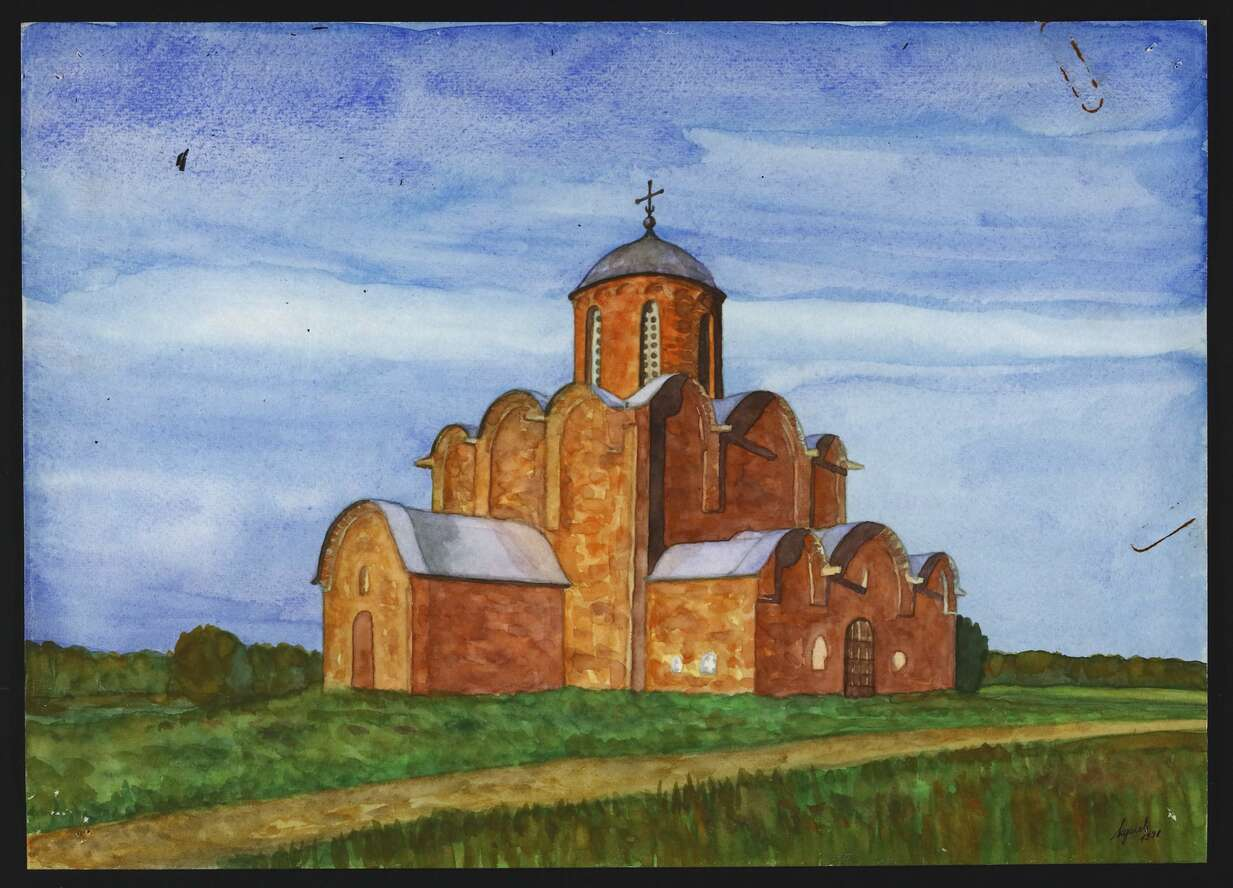
\includegraphics[width=0.45\textwidth]{images/style_augments/1998_14-17_0101_RUS_R_C.jpg}\hfil
        %  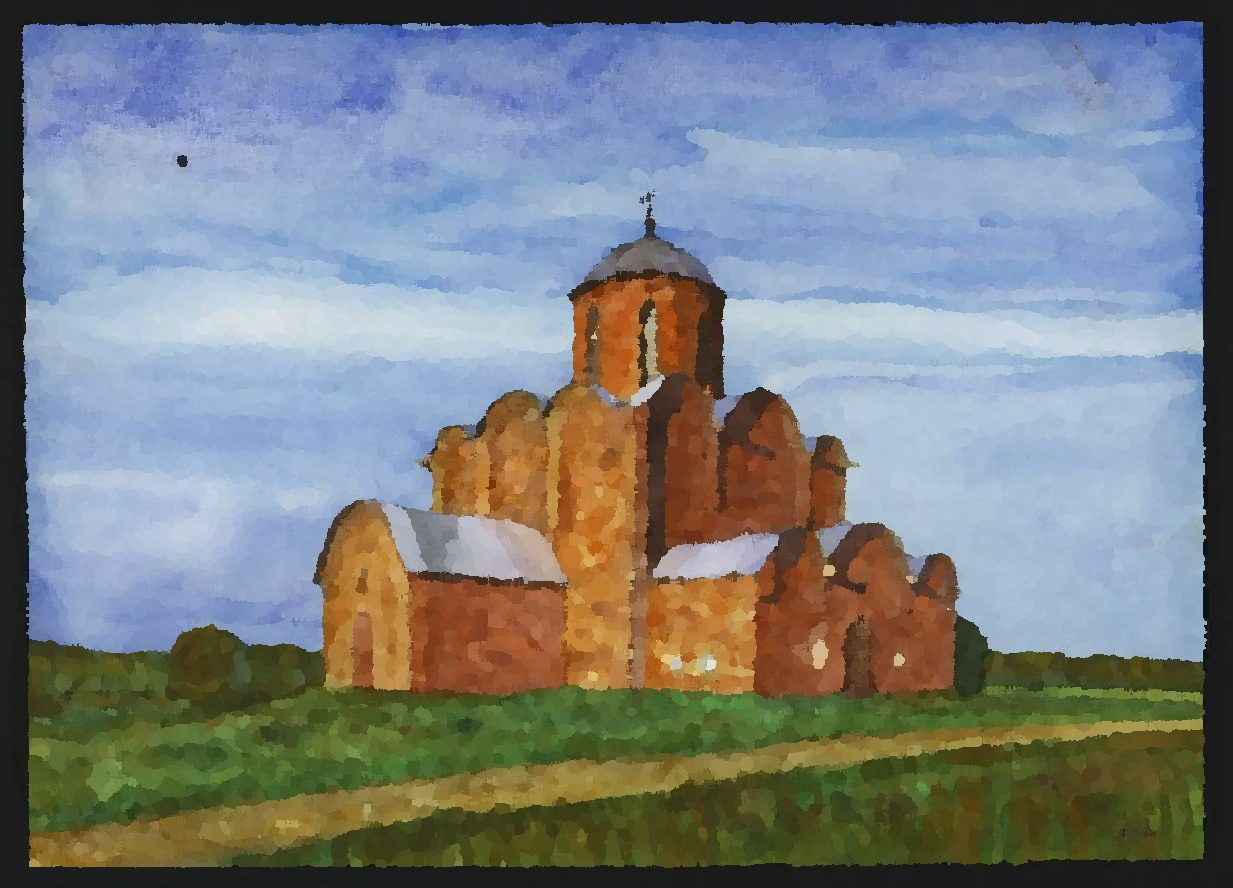
\includegraphics[width=0.45\textwidth]{images/style_augments/1998_14-17_0101_RUS_R_C_oil.jpg}
         \caption{}
     \end{subfigure}
     \hfil
     \begin{subfigure}[b]{0.5\textwidth}
         \centering
         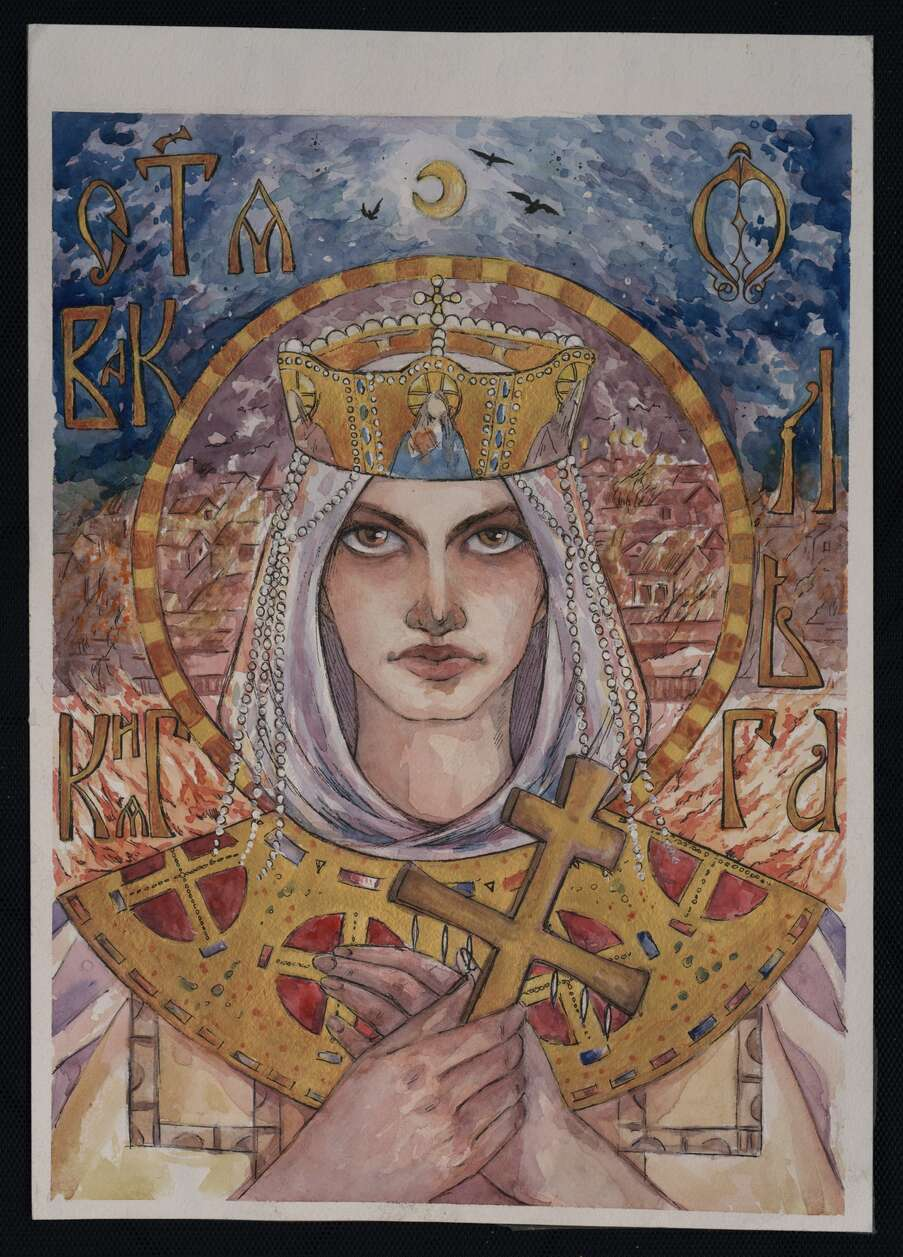
\includegraphics[width=0.45\textwidth]{images/style_augments/2019_14-17_0193_RUS_R_C.jpg}\hfil
         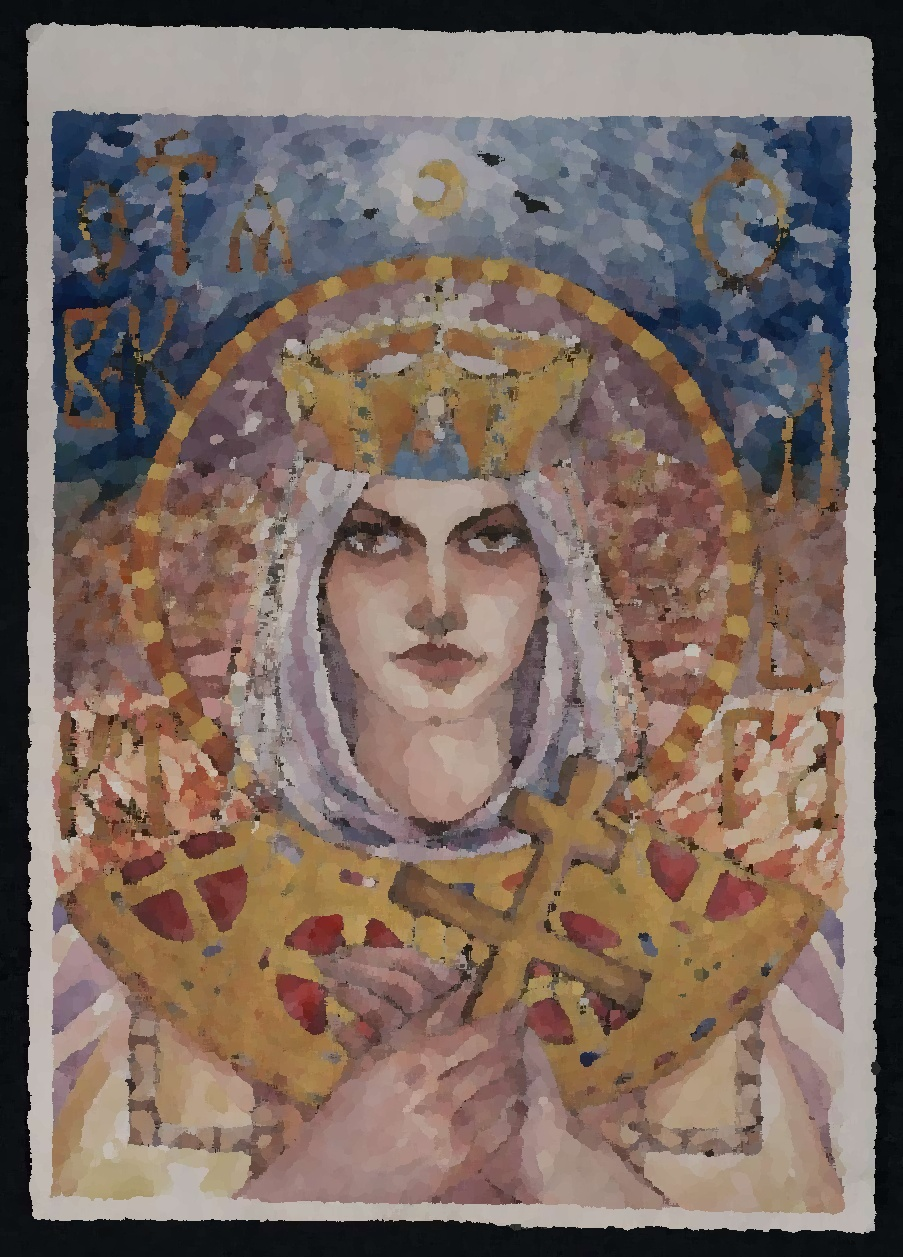
\includegraphics[width=0.45\textwidth]{images/style_augments/2019_14-17_0193_RUS_R_C_oil.jpg}
         \caption{}
     \end{subfigure}
     \hfil
     \begin{subfigure}[b]{0.5\textwidth}
         \centering
         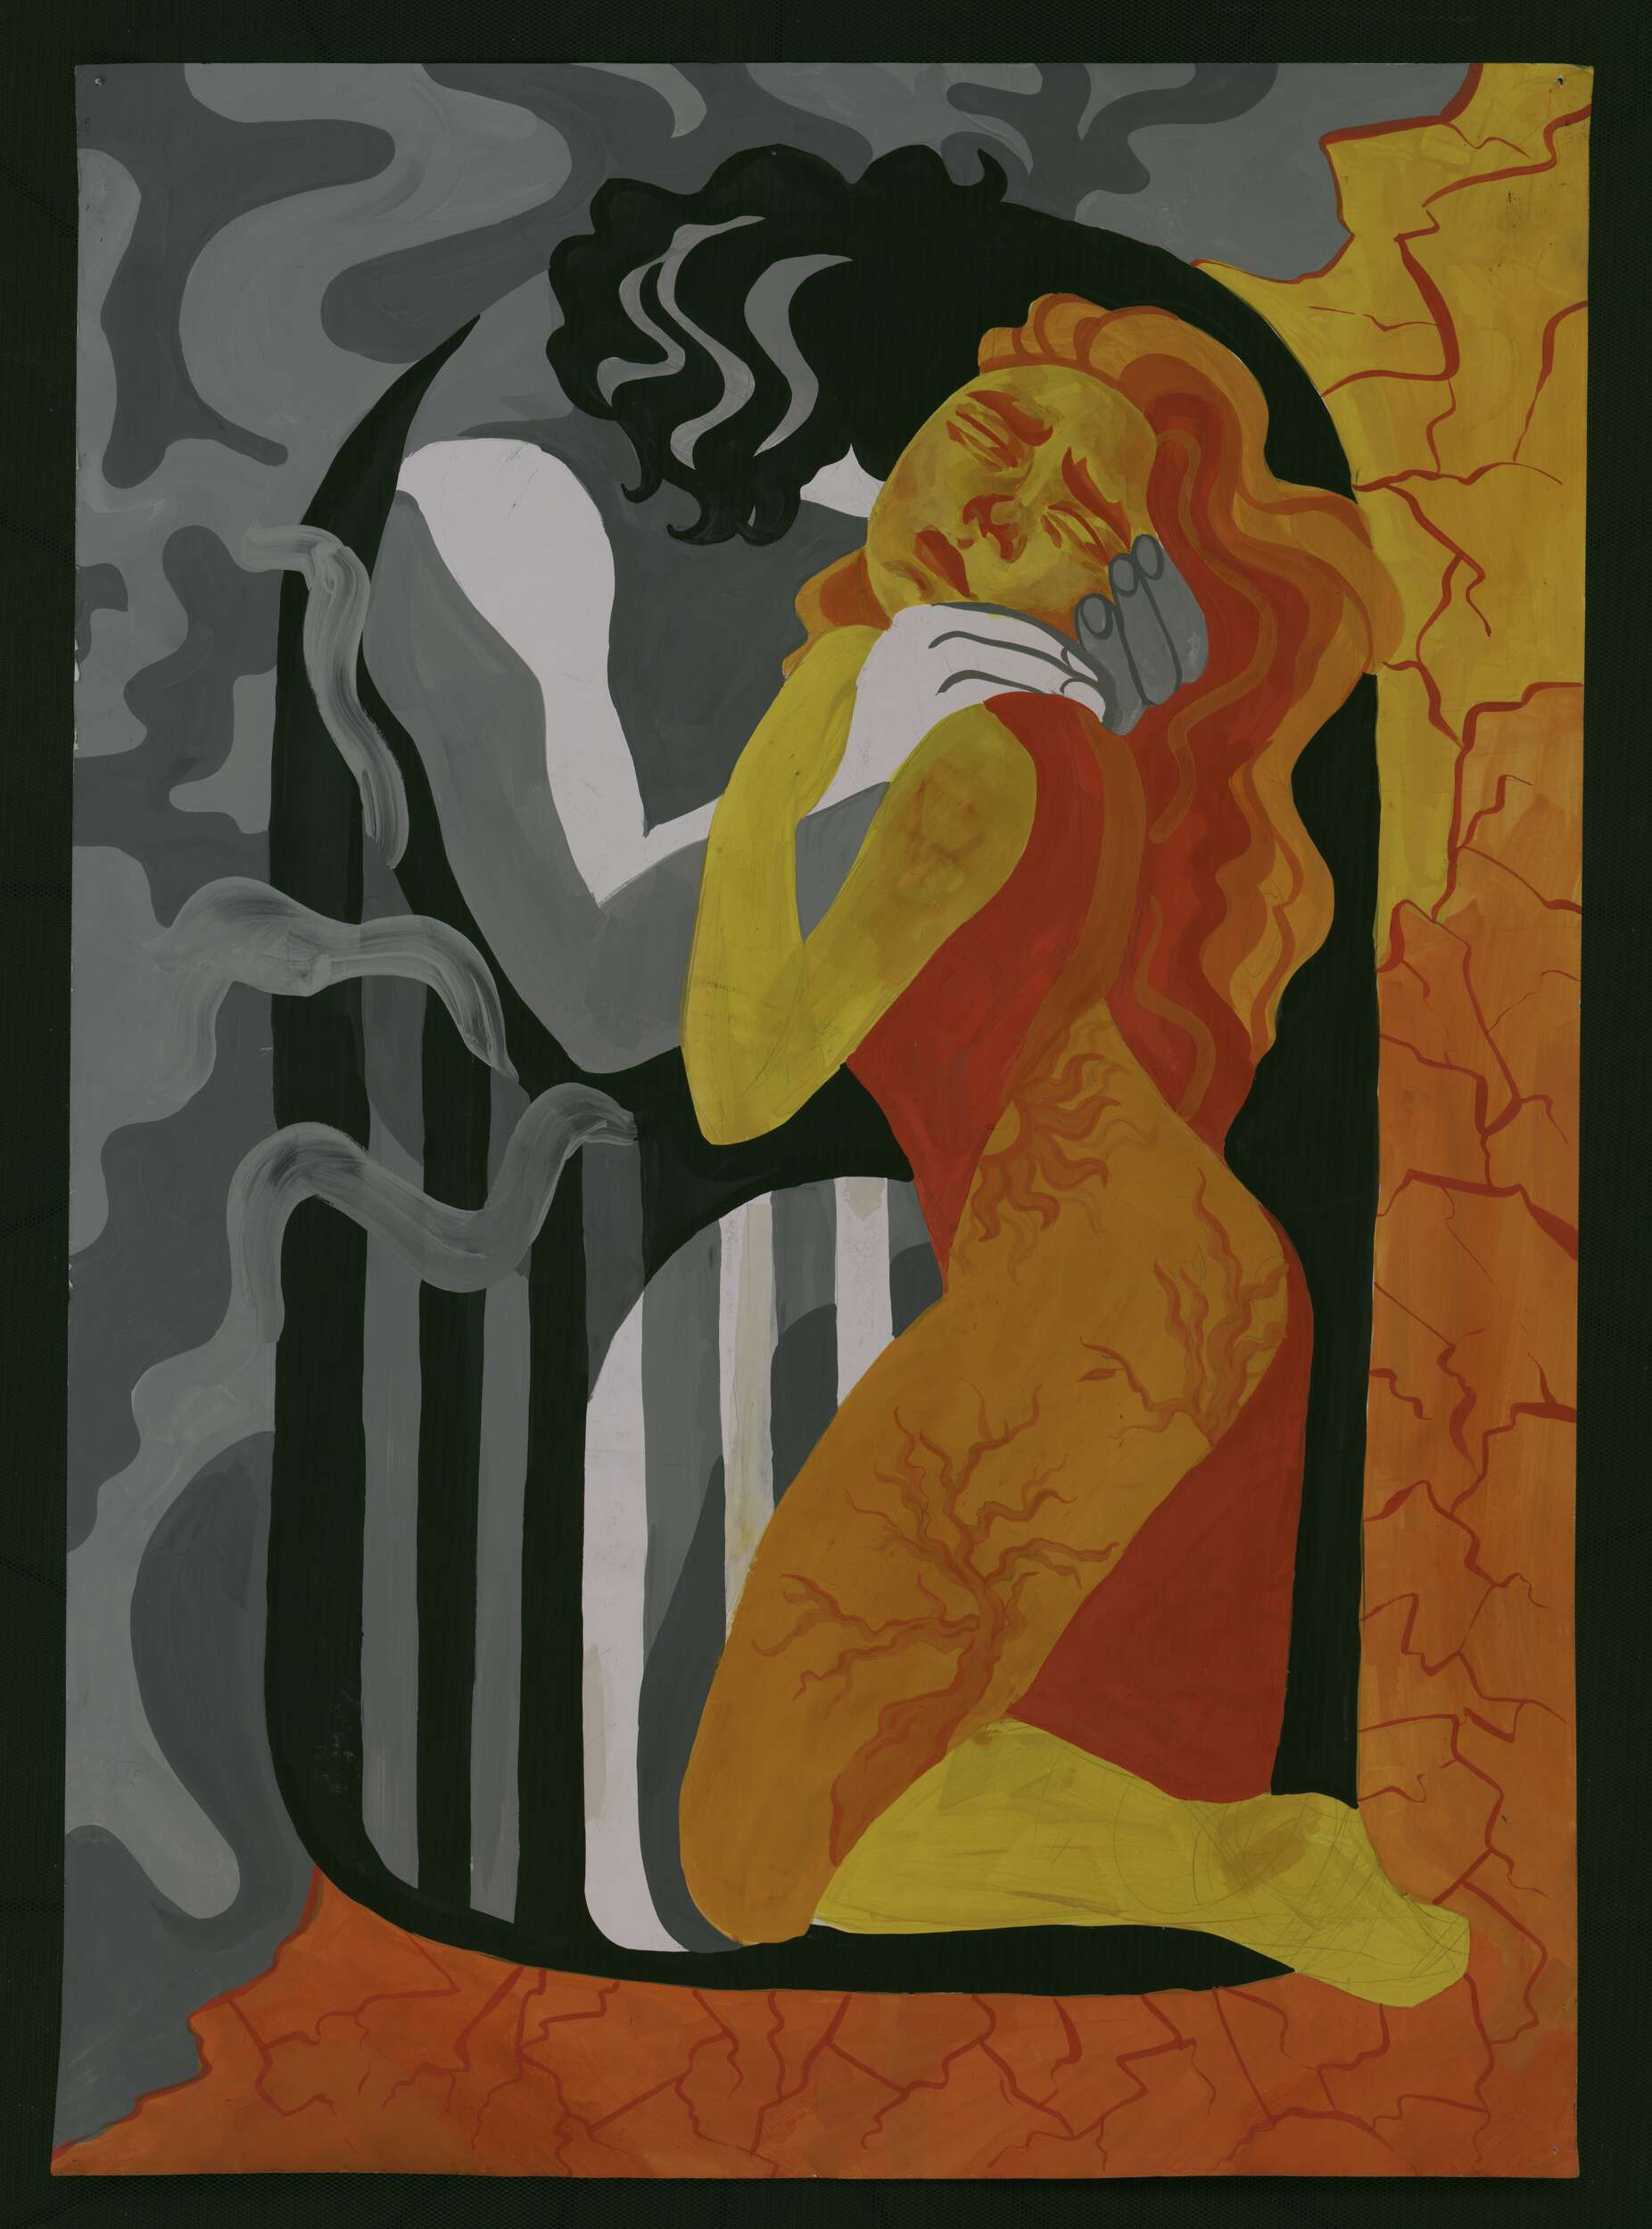
\includegraphics[width=0.45\textwidth]{images/style_augments/2020_14-17_2051_UKR_R_C.jpg}\hfil
         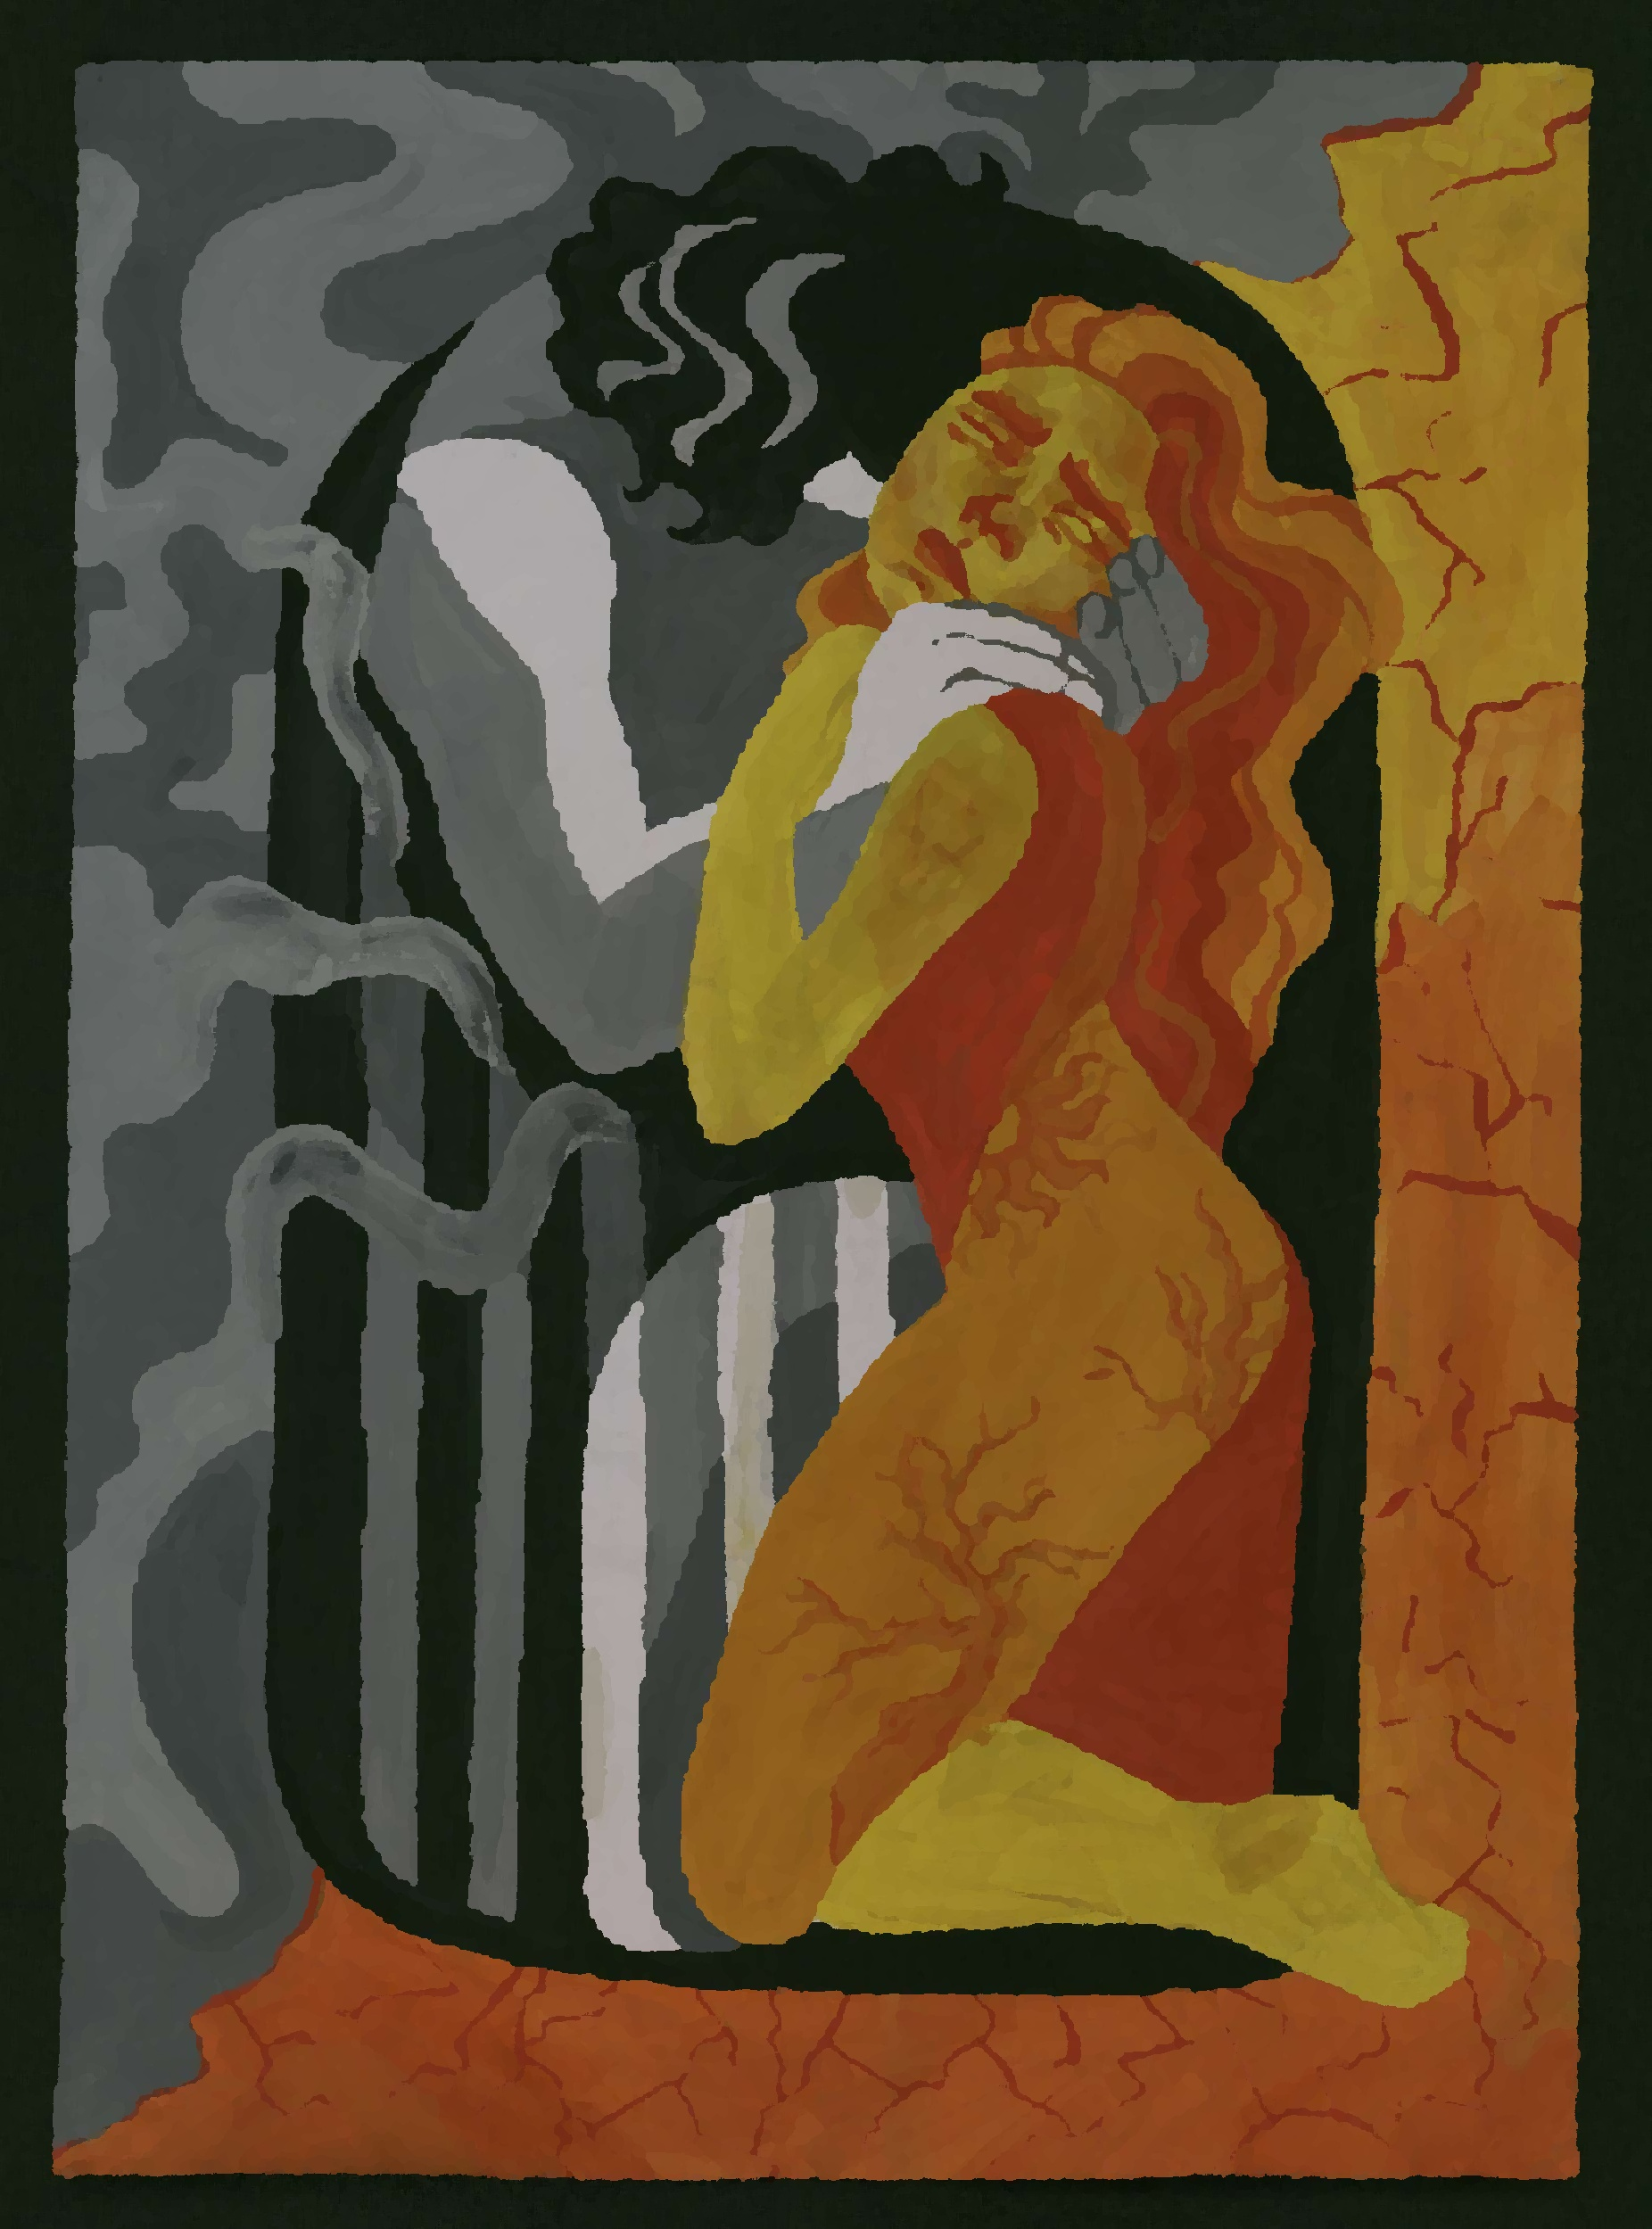
\includegraphics[width=0.45\textwidth]{images/style_augments/2020_14-17_2051_UKR_R_C_oil.jpg}
         \caption{}
     \end{subfigure}
     \hfil
     \begin{subfigure}[b]{0.5\textwidth}
         \centering
         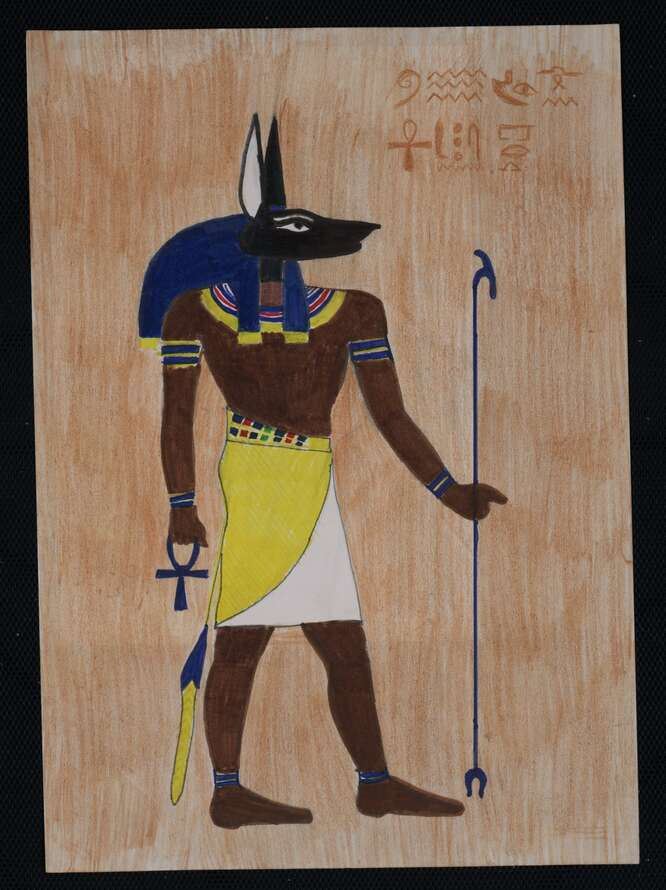
\includegraphics[width=0.45\textwidth]{images/style_augments/2019_14-17_0188_RUS_R_C.jpg}\hfil
         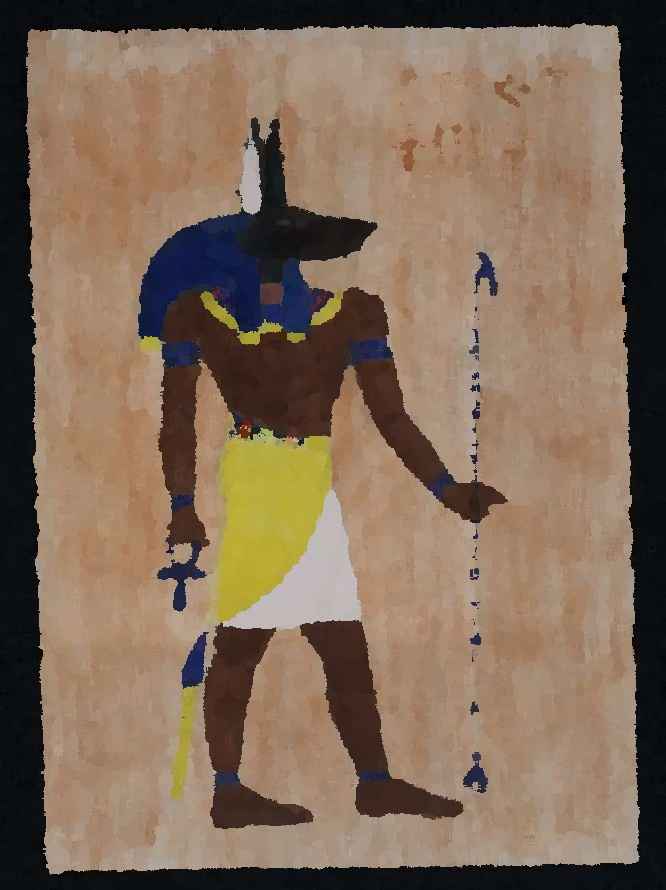
\includegraphics[width=0.45\textwidth]{images/style_augments/2019_14-17_0188_RUS_R_C_oil.jpg}
         \caption{}
     \end{subfigure}
     \caption{Examples of drawings (on left) after apply oil painting effect (on right)}
     \label{fig:oil-style-effects}
\end{figure}


\begin{figure}
     \centering
     \begin{subfigure}[b]{0.5\textwidth}
         \centering
         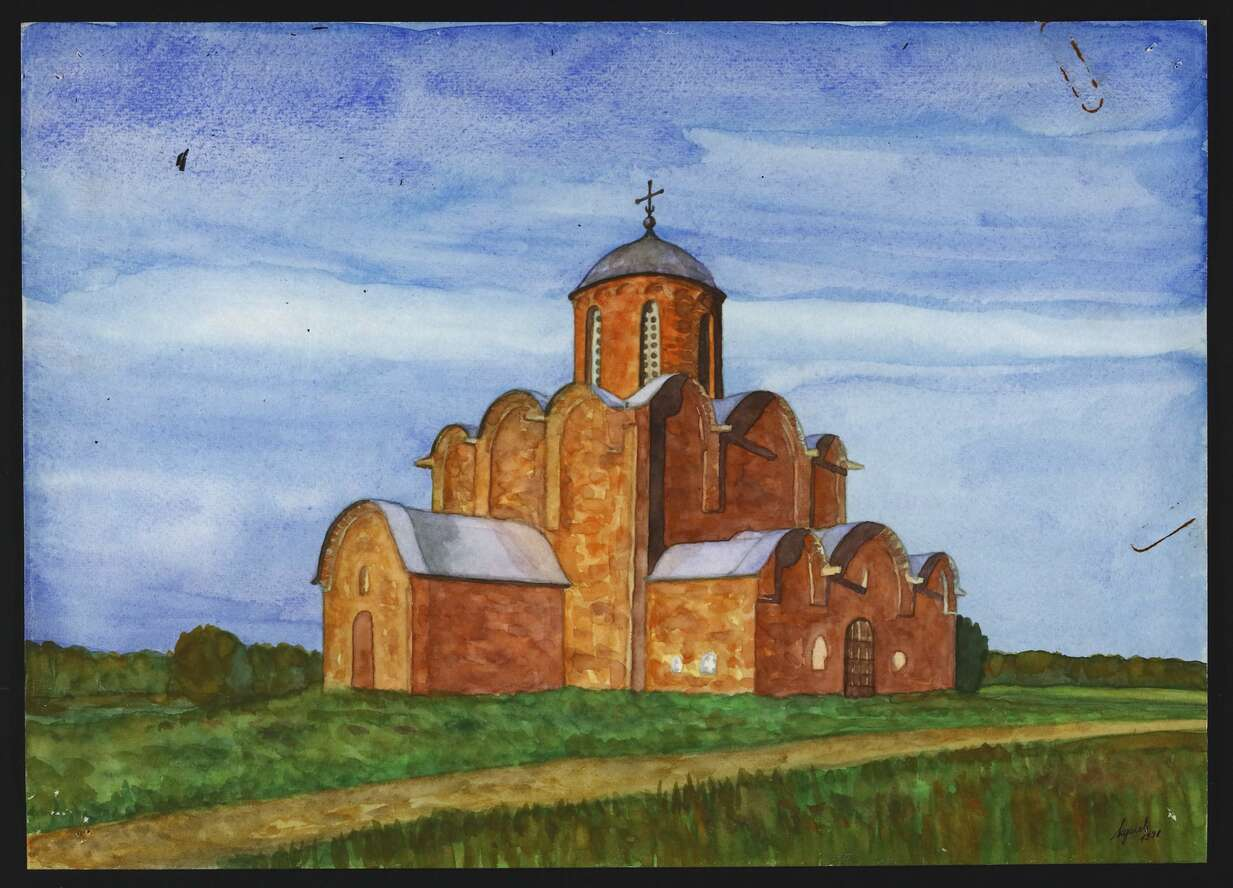
\includegraphics[width=0.45\textwidth]{images/style_augments/1998_14-17_0101_RUS_R_C.jpg}\hfil
         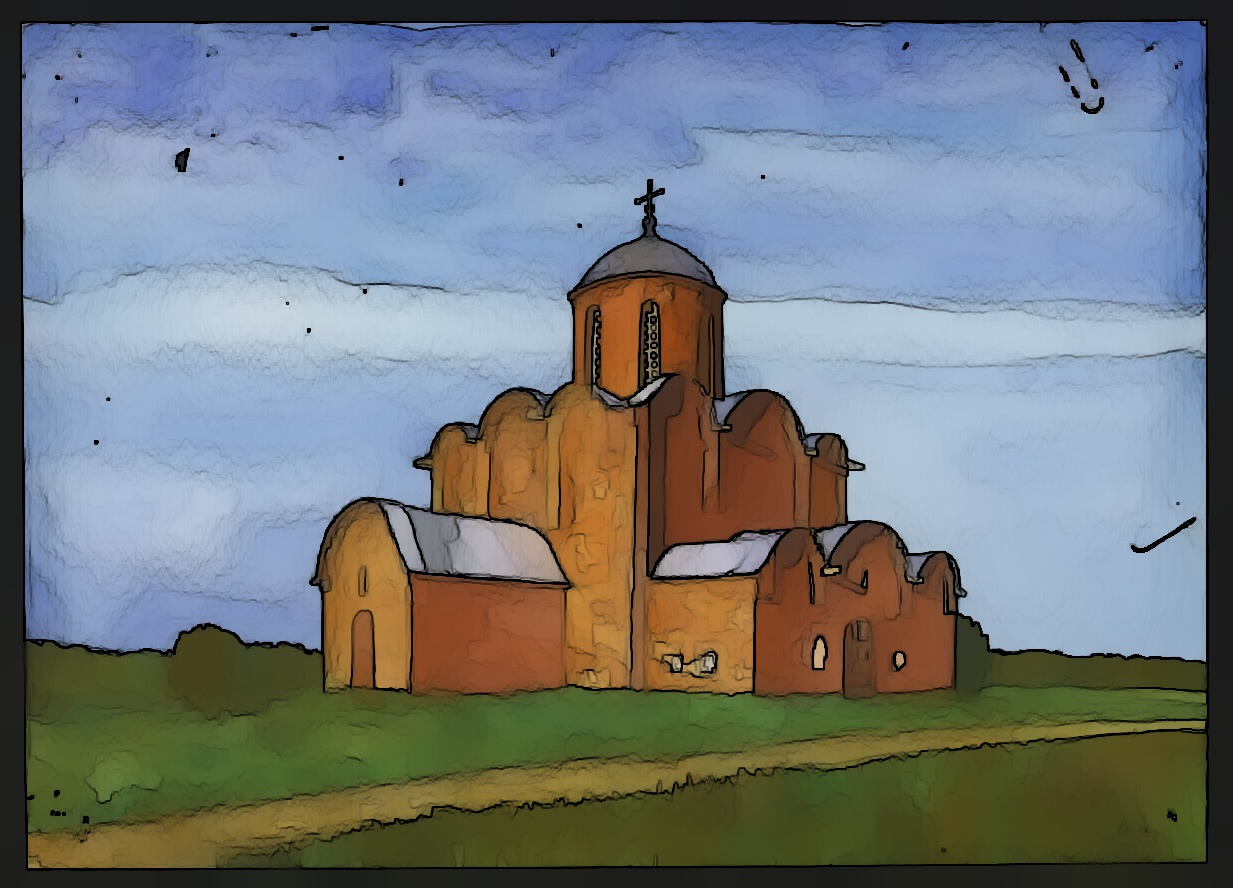
\includegraphics[width=0.45\textwidth]{images/style_augments/1998_14-17_0101_RUS_R_C_water.jpg}
         \caption{}
     \end{subfigure}
     \hfil
     \begin{subfigure}[b]{0.5\textwidth}
         \centering
         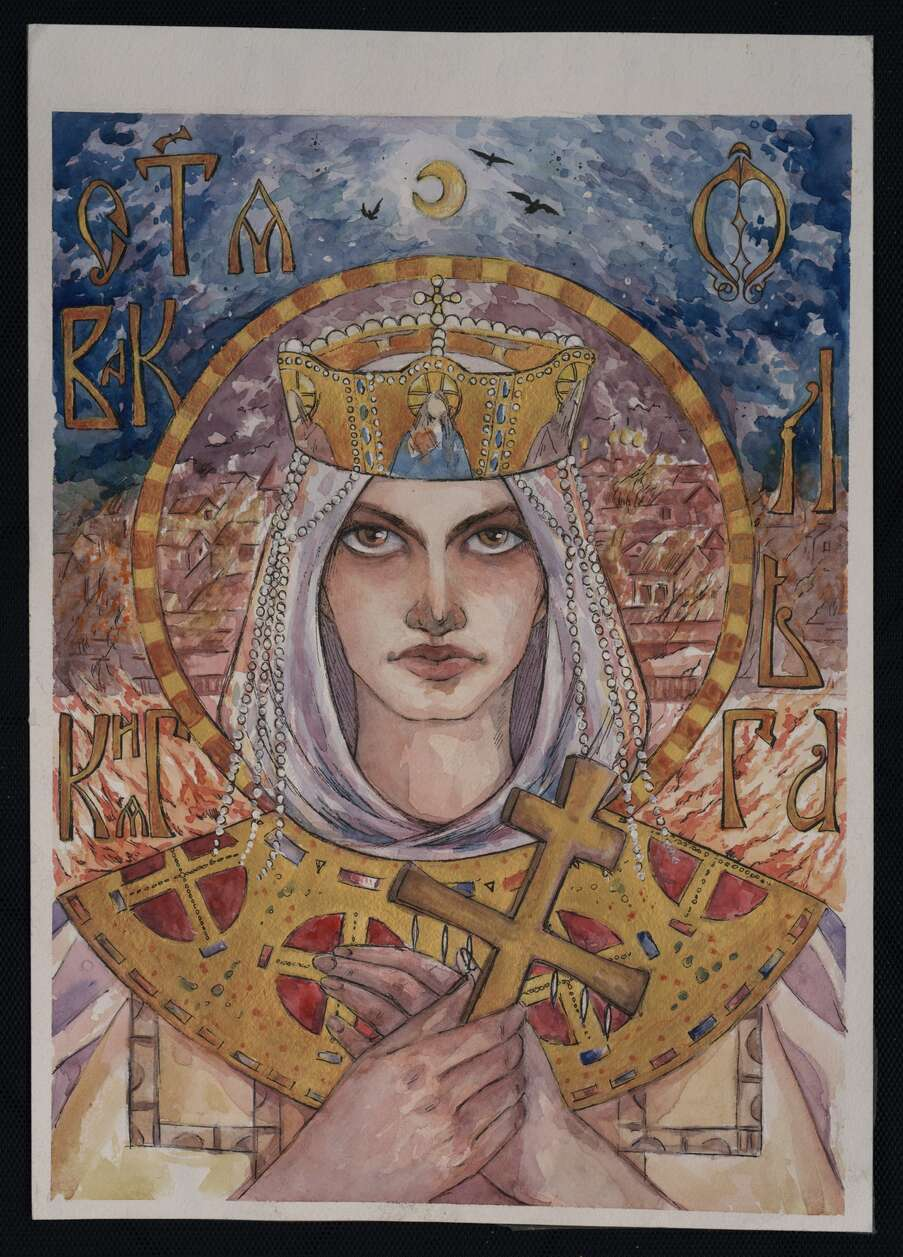
\includegraphics[width=0.45\textwidth]{images/style_augments/2019_14-17_0193_RUS_R_C.jpg}\hfil
         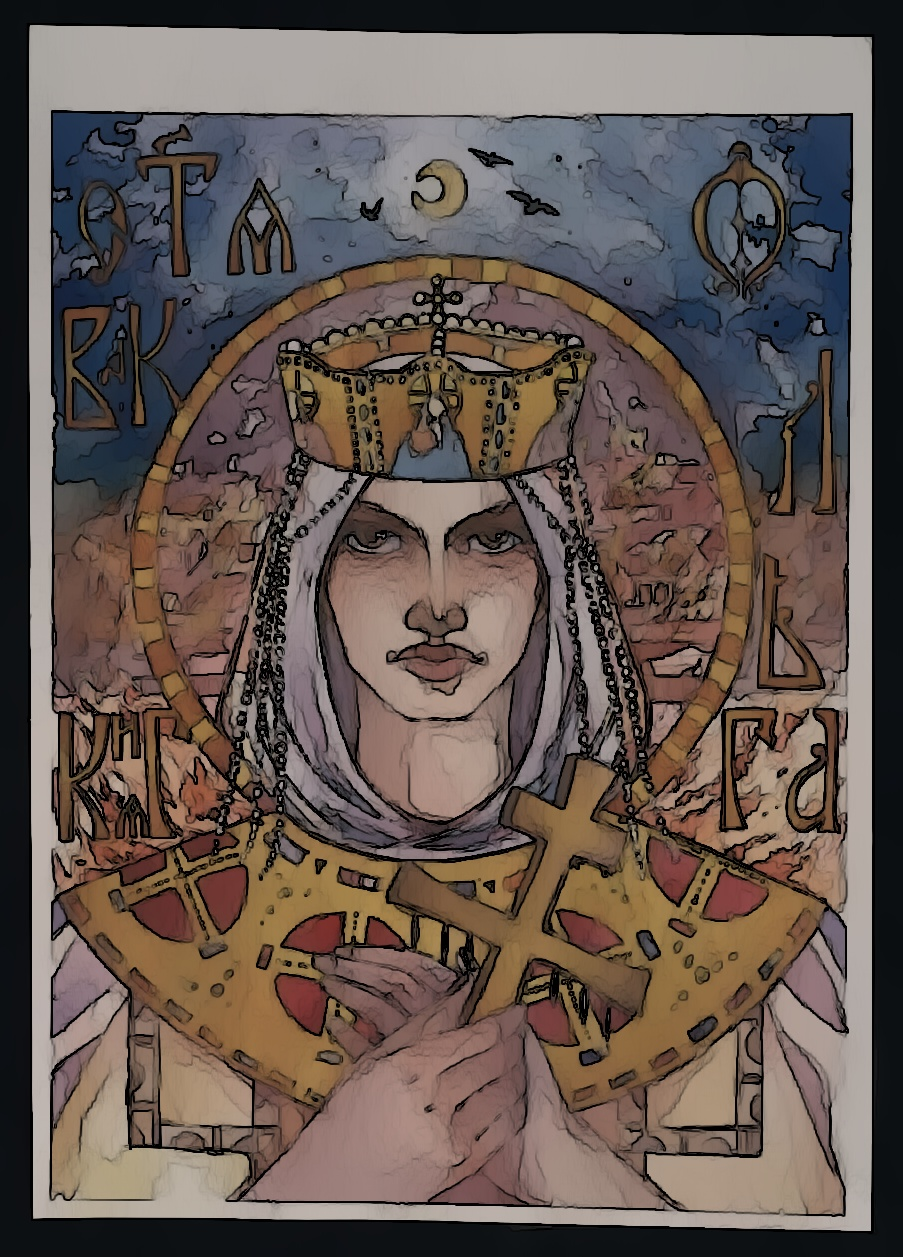
\includegraphics[width=0.45\textwidth]{images/style_augments/2019_14-17_0193_RUS_R_C_water.jpg}
         \caption{}
     \end{subfigure}
     \hfil
     \begin{subfigure}[b]{0.5\textwidth}
         \centering
         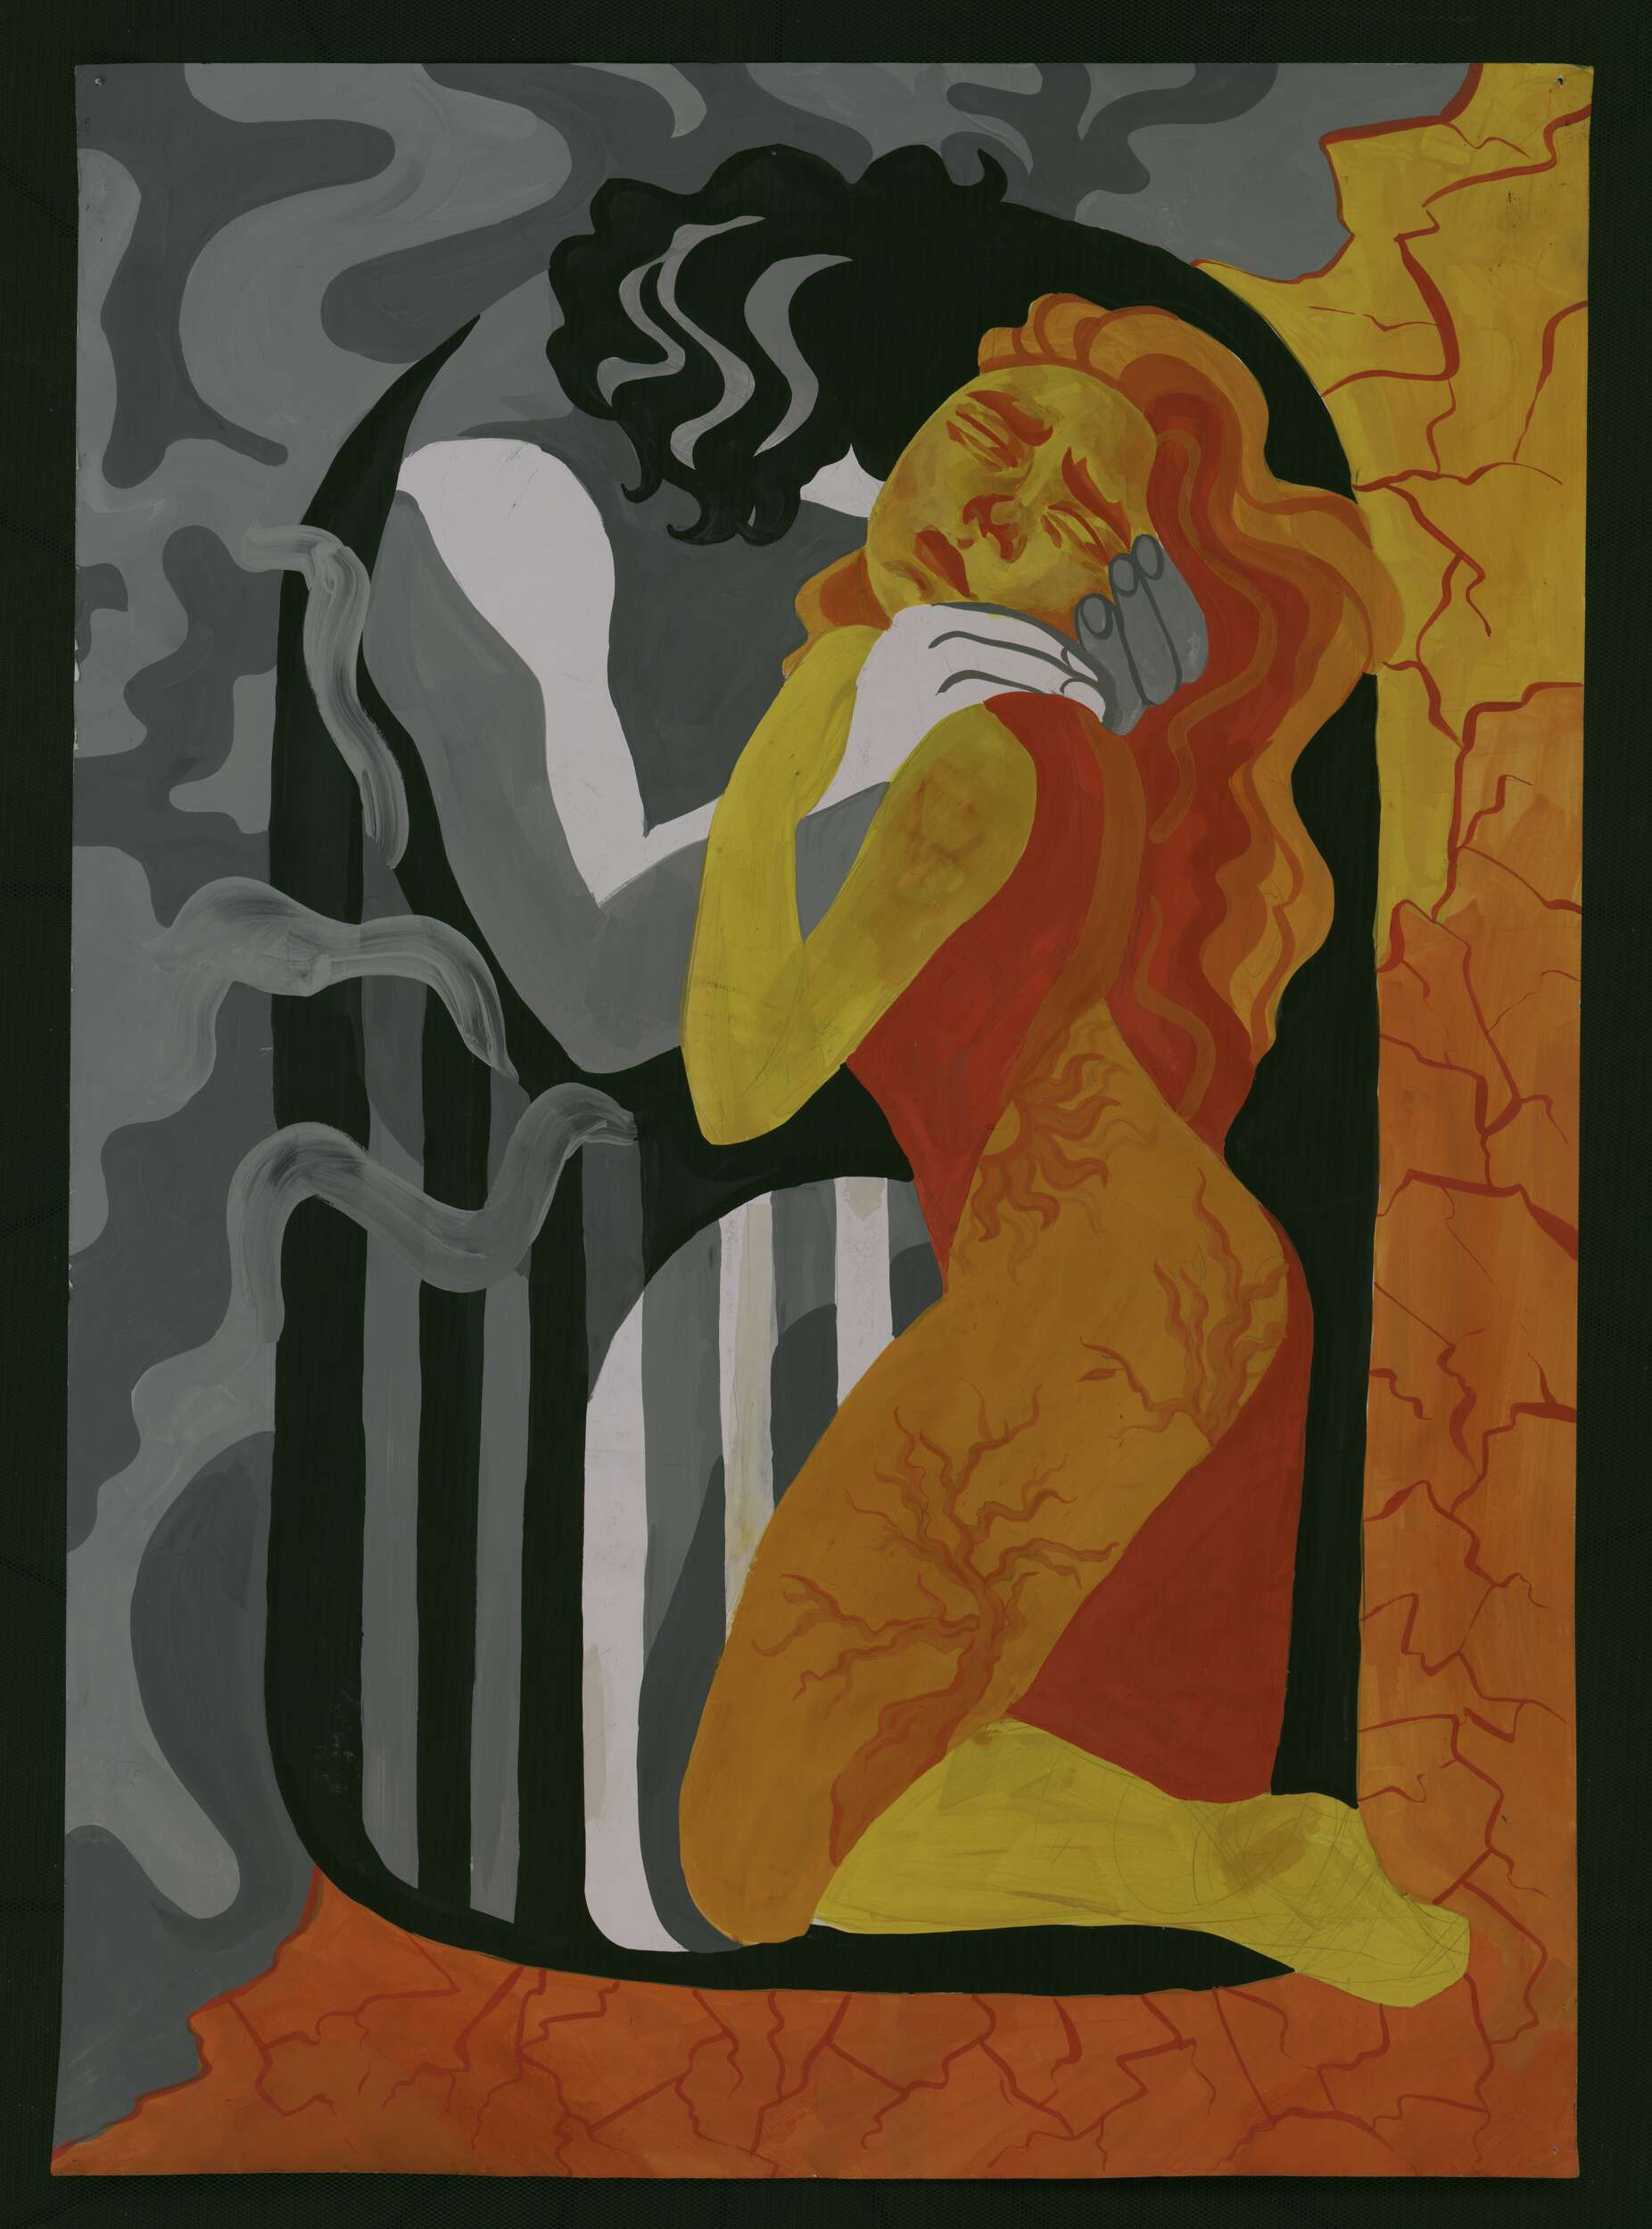
\includegraphics[width=0.45\textwidth]{images/style_augments/2020_14-17_2051_UKR_R_C.jpg}\hfil
         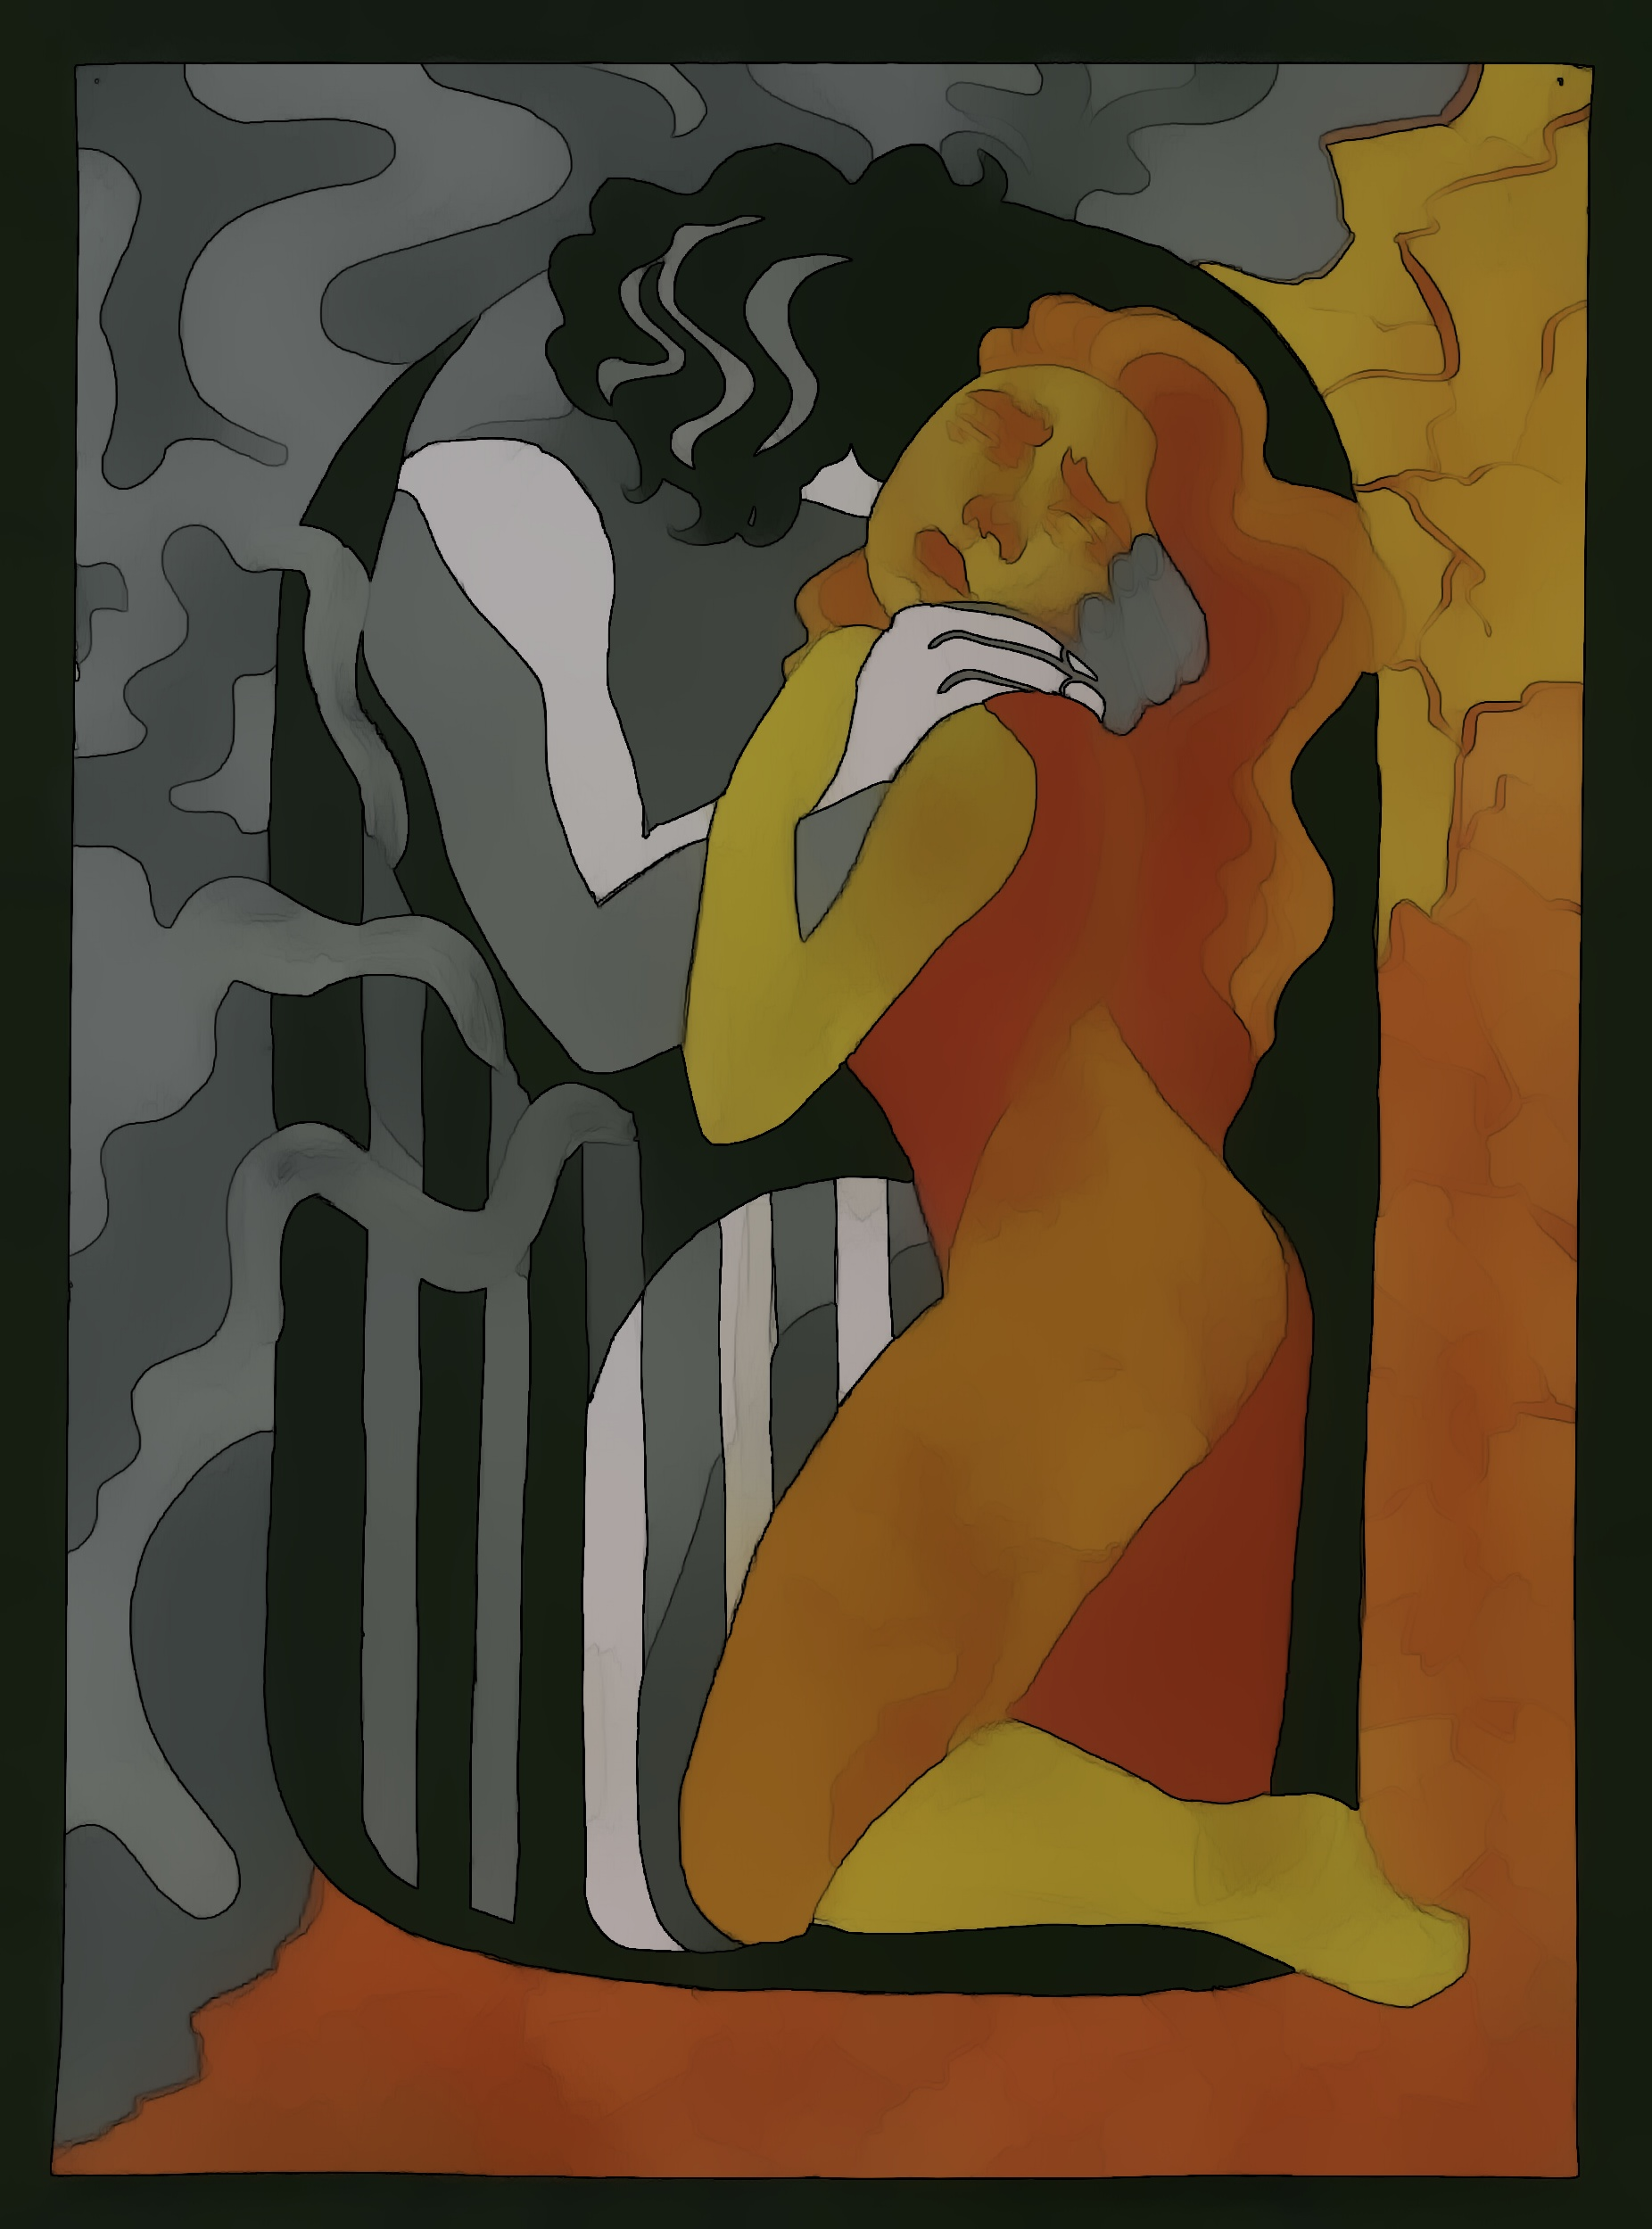
\includegraphics[width=0.45\textwidth]{images/style_augments/2020_14-17_2051_UKR_R_C_water.jpg}
         \caption{}
     \end{subfigure}
     \hfil
     \begin{subfigure}[b]{0.5\textwidth}
         \centering
         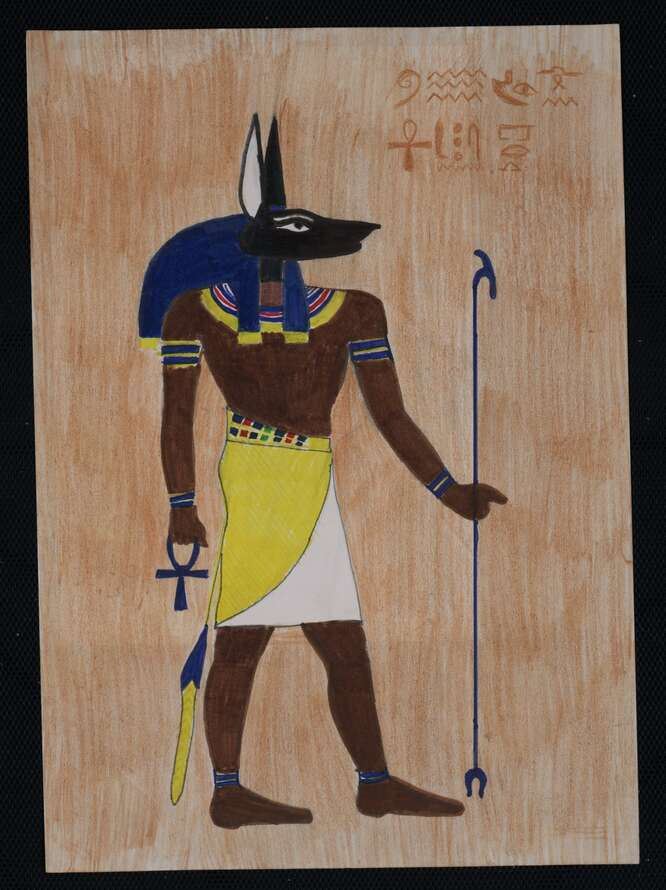
\includegraphics[width=0.45\textwidth]{images/style_augments/2019_14-17_0188_RUS_R_C.jpg}\hfil
         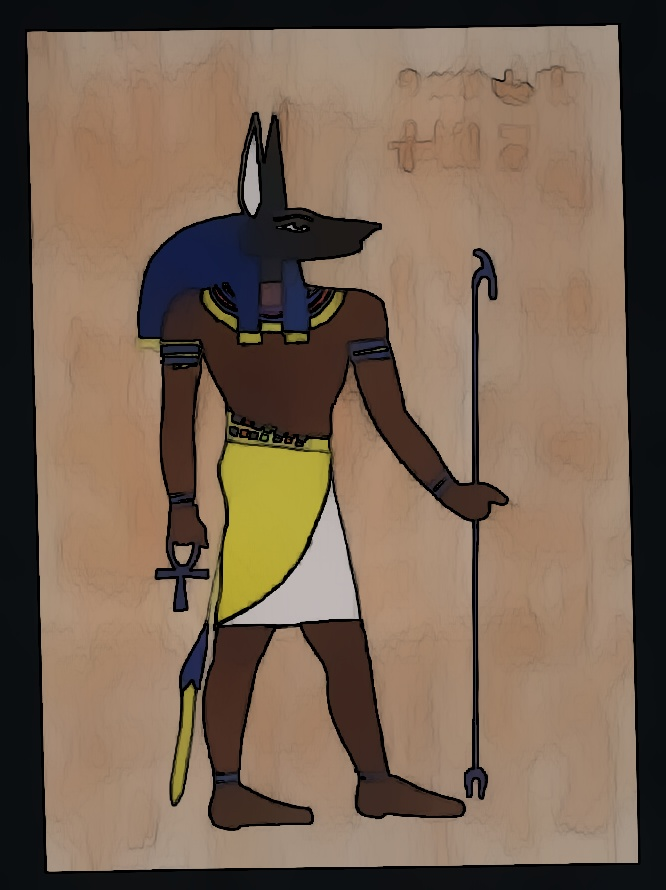
\includegraphics[width=0.45\textwidth]{images/style_augments/2019_14-17_0188_RUS_R_C_water.jpg}
         \caption{}
     \end{subfigure}
     \caption{Examples of drawings (on left) after apply watercolor effect (on right)}
     \label{fig:water-style-effects}
\end{figure}


\begin{figure}
     \centering
     \begin{subfigure}[b]{0.5\textwidth}
         \centering
         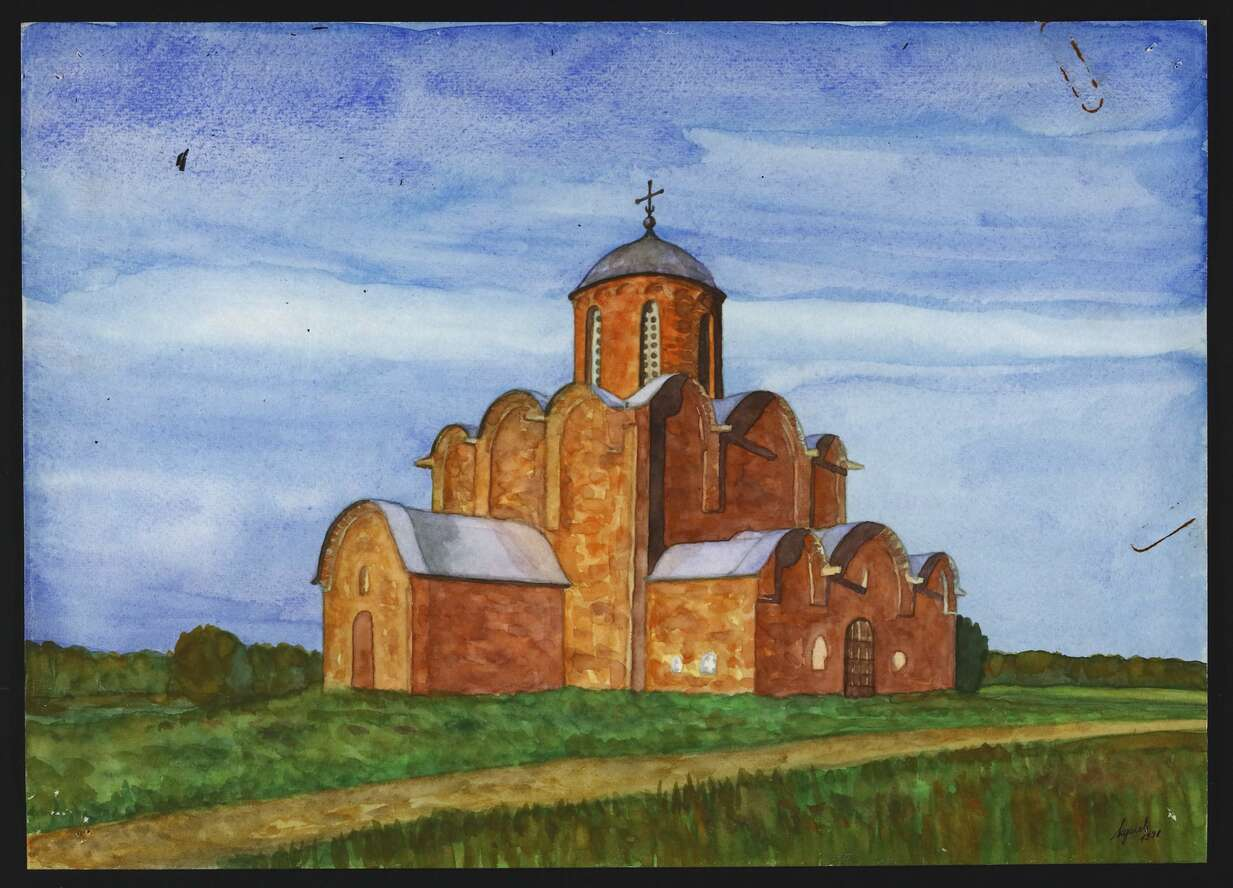
\includegraphics[width=0.45\textwidth]{images/style_augments/1998_14-17_0101_RUS_R_C.jpg}\hfil
         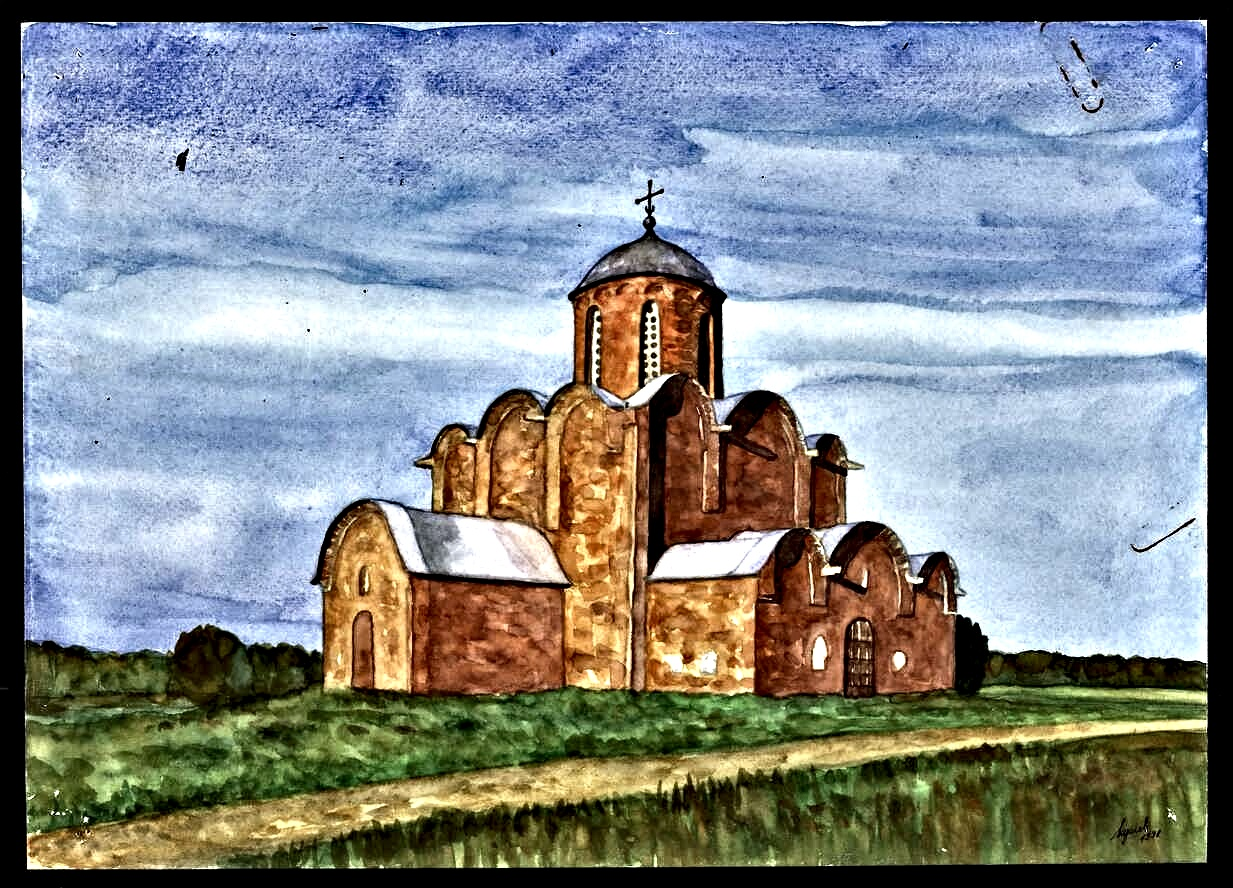
\includegraphics[width=0.45\textwidth]{images/style_augments/1998_14-17_0101_RUS_R_C_texture.jpg}
         \caption{}
     \end{subfigure}
     \hfil
     \begin{subfigure}[b]{0.5\textwidth}
         \centering
         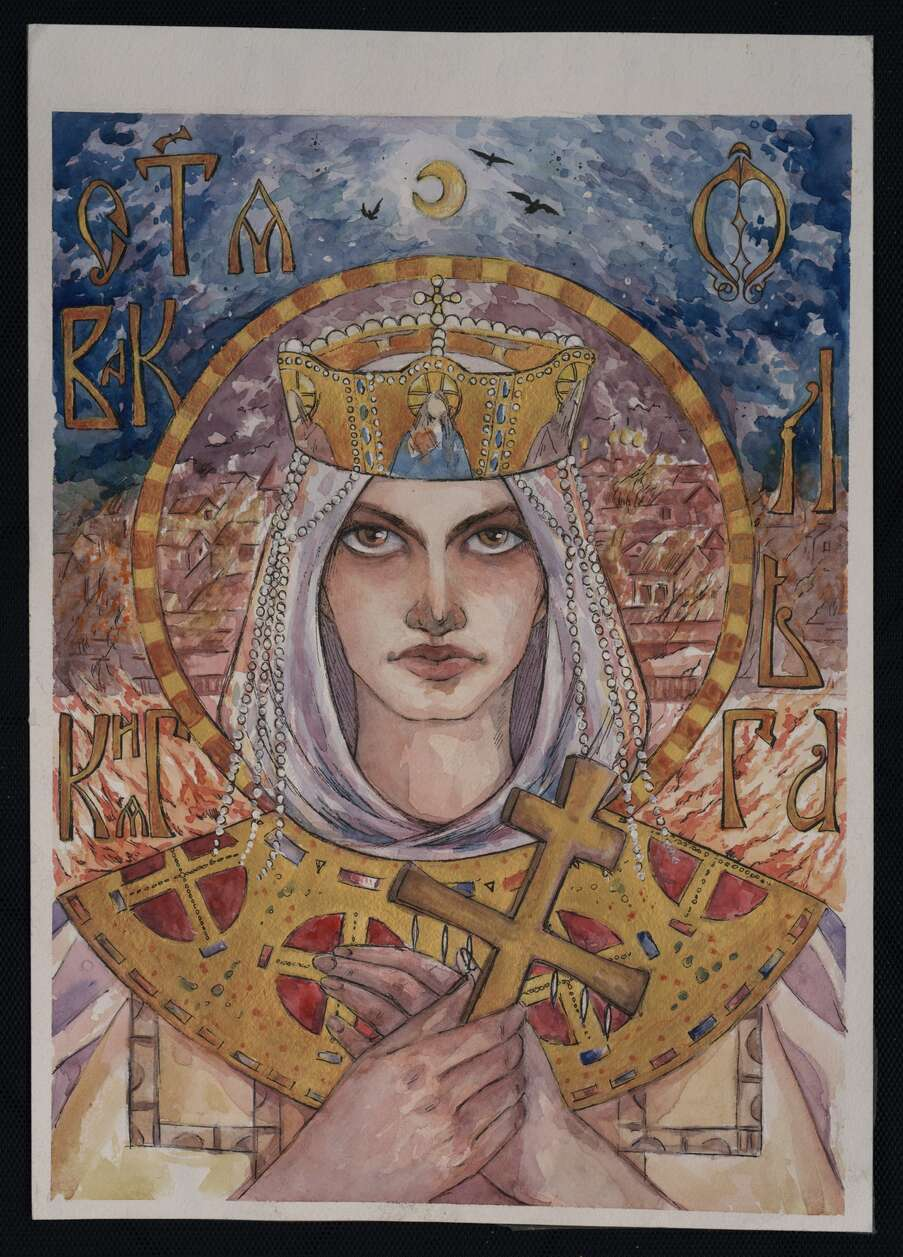
\includegraphics[width=0.45\textwidth]{images/style_augments/2019_14-17_0193_RUS_R_C.jpg}\hfil
         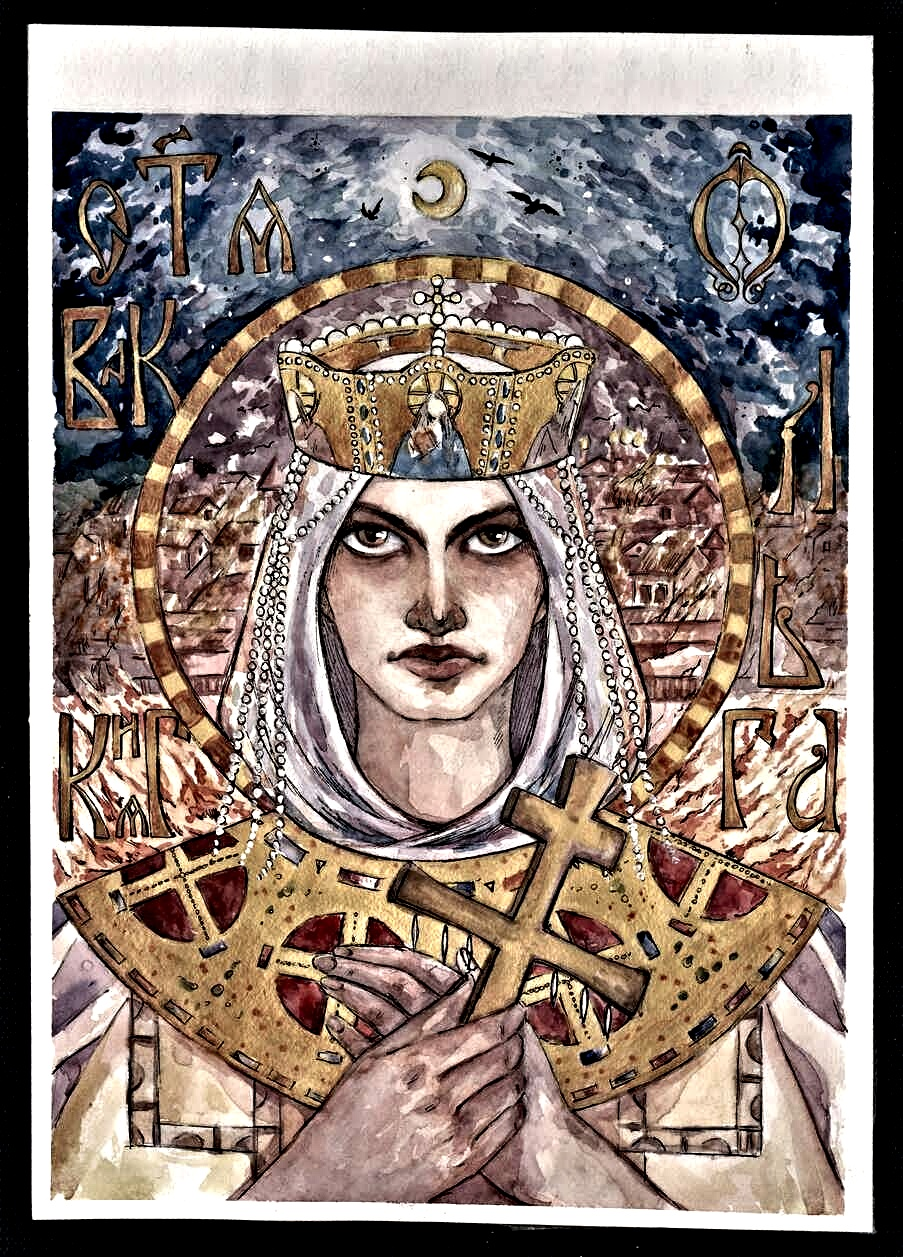
\includegraphics[width=0.45\textwidth]{images/style_augments/2019_14-17_0193_RUS_R_C_texture.jpg}
         \caption{}
     \end{subfigure}
     \hfil
     \begin{subfigure}[b]{0.5\textwidth}
         \centering
         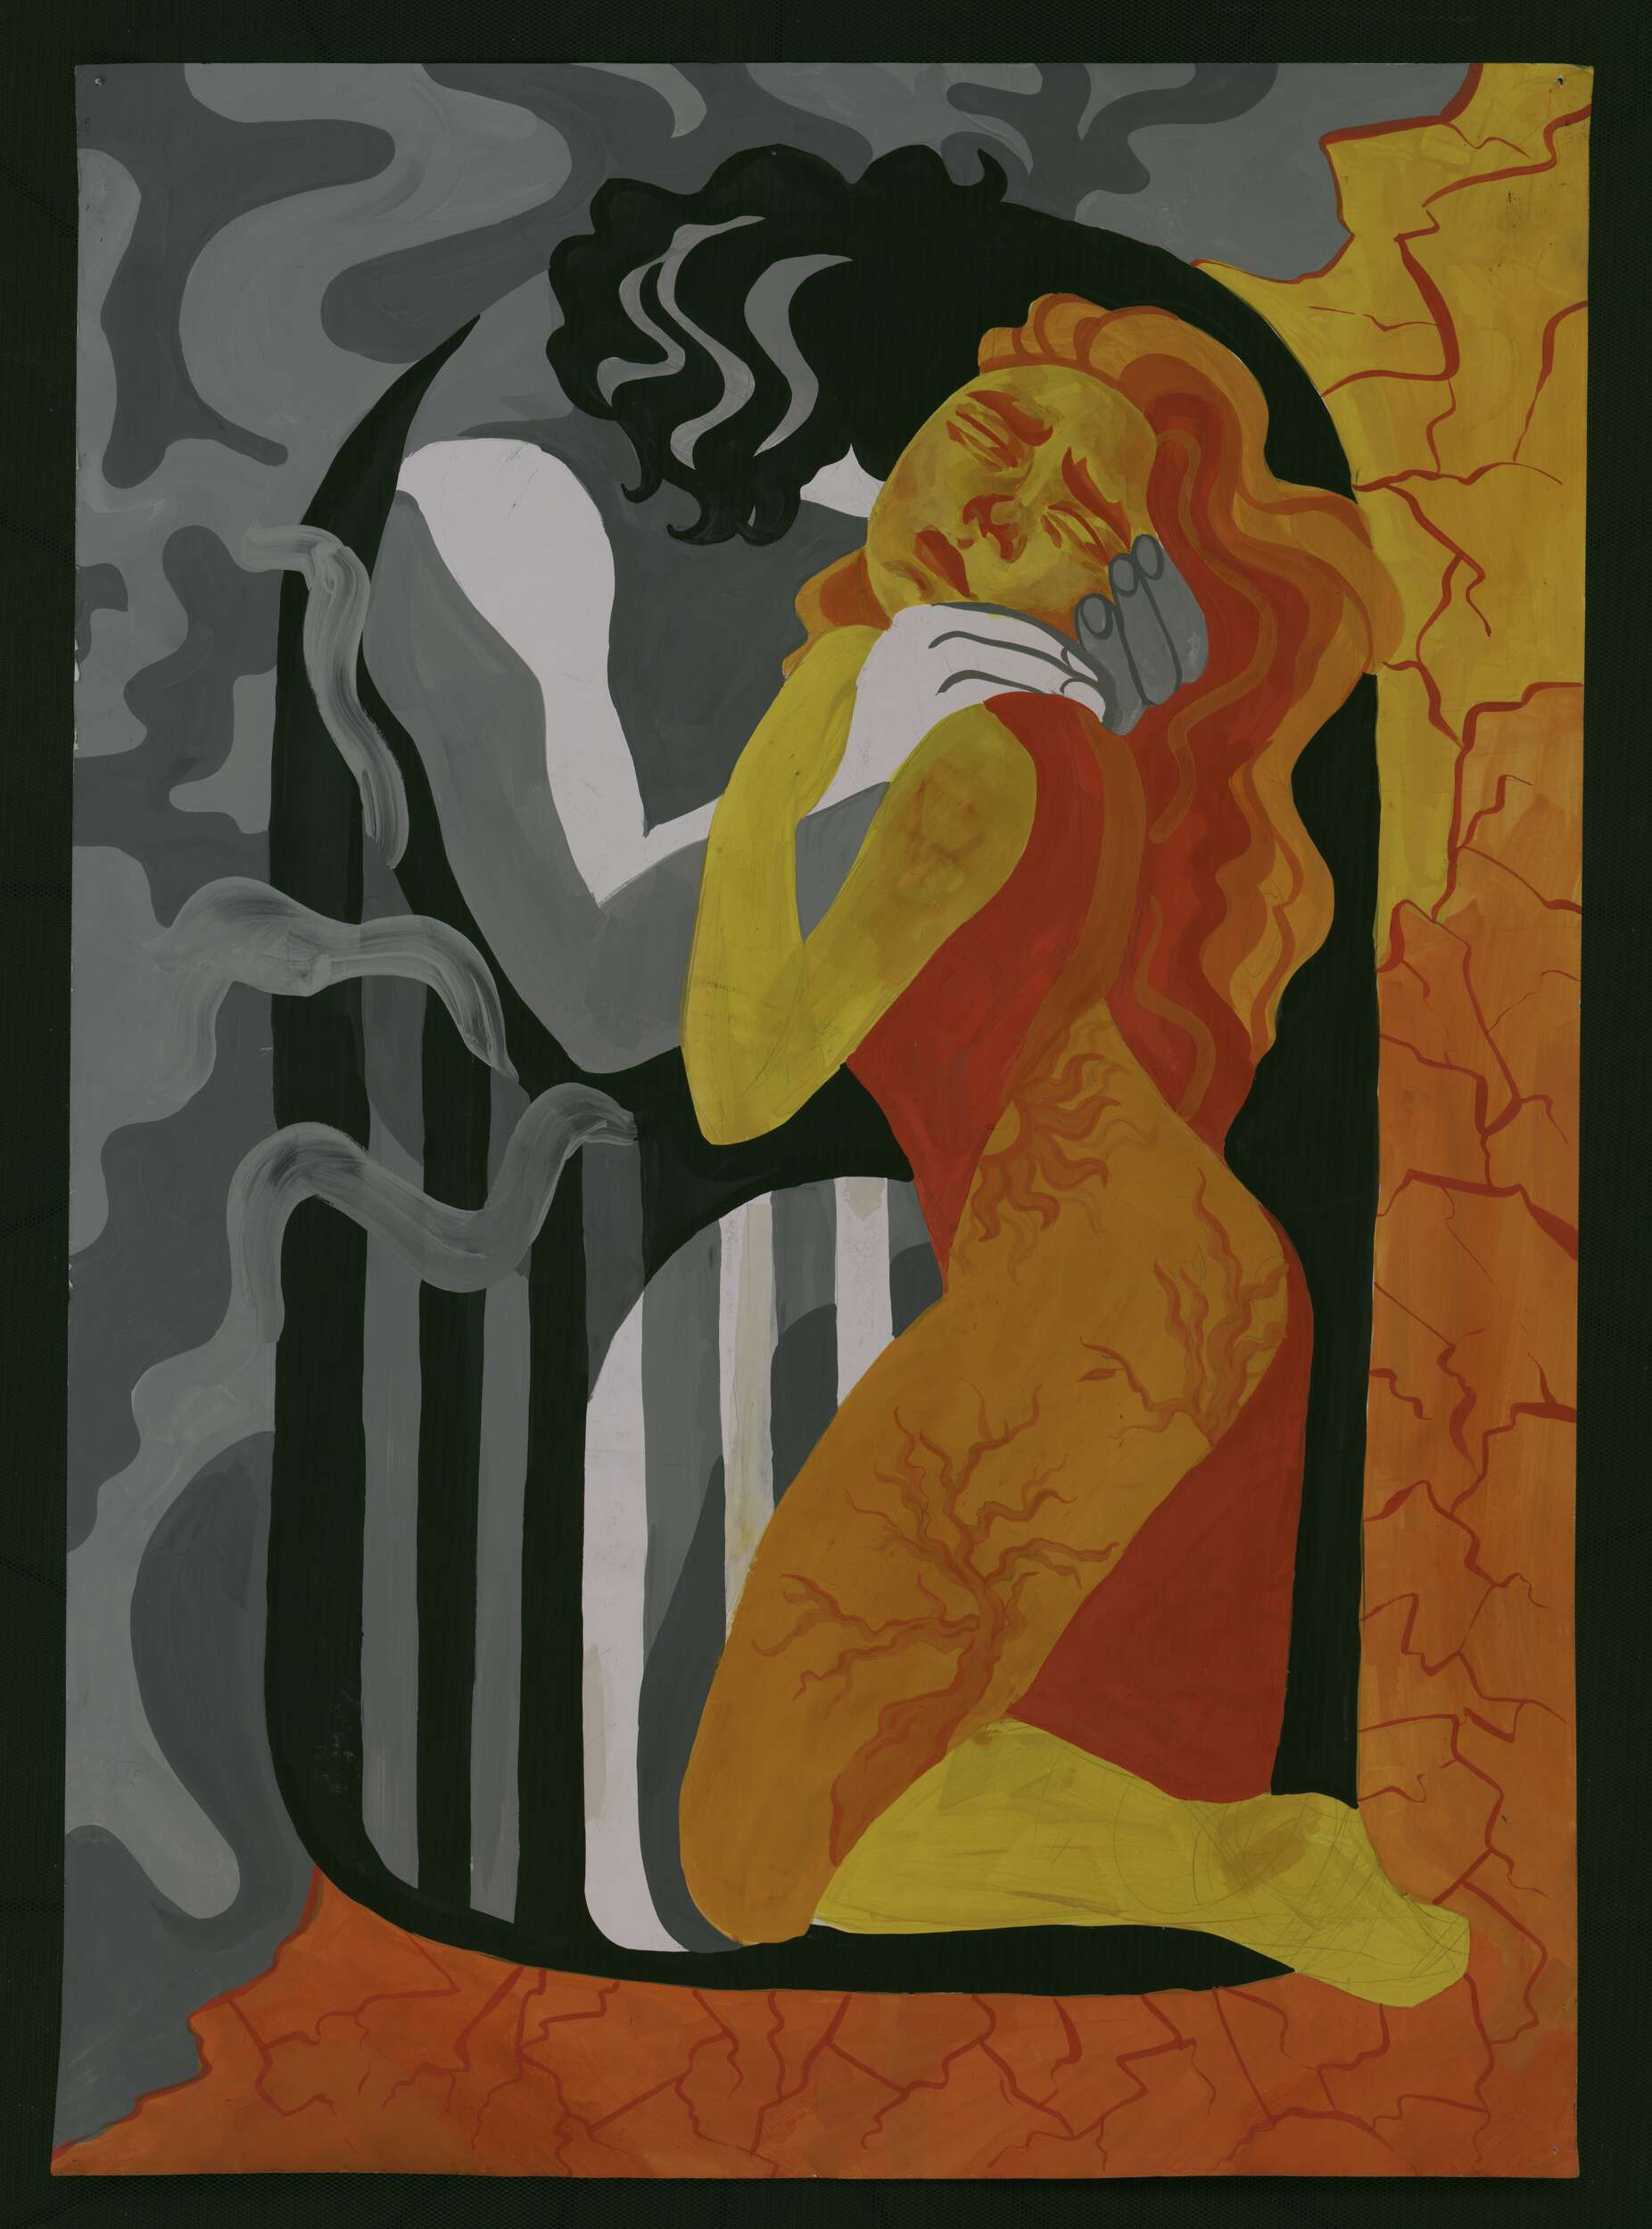
\includegraphics[width=0.45\textwidth]{images/style_augments/2020_14-17_2051_UKR_R_C.jpg}\hfil
         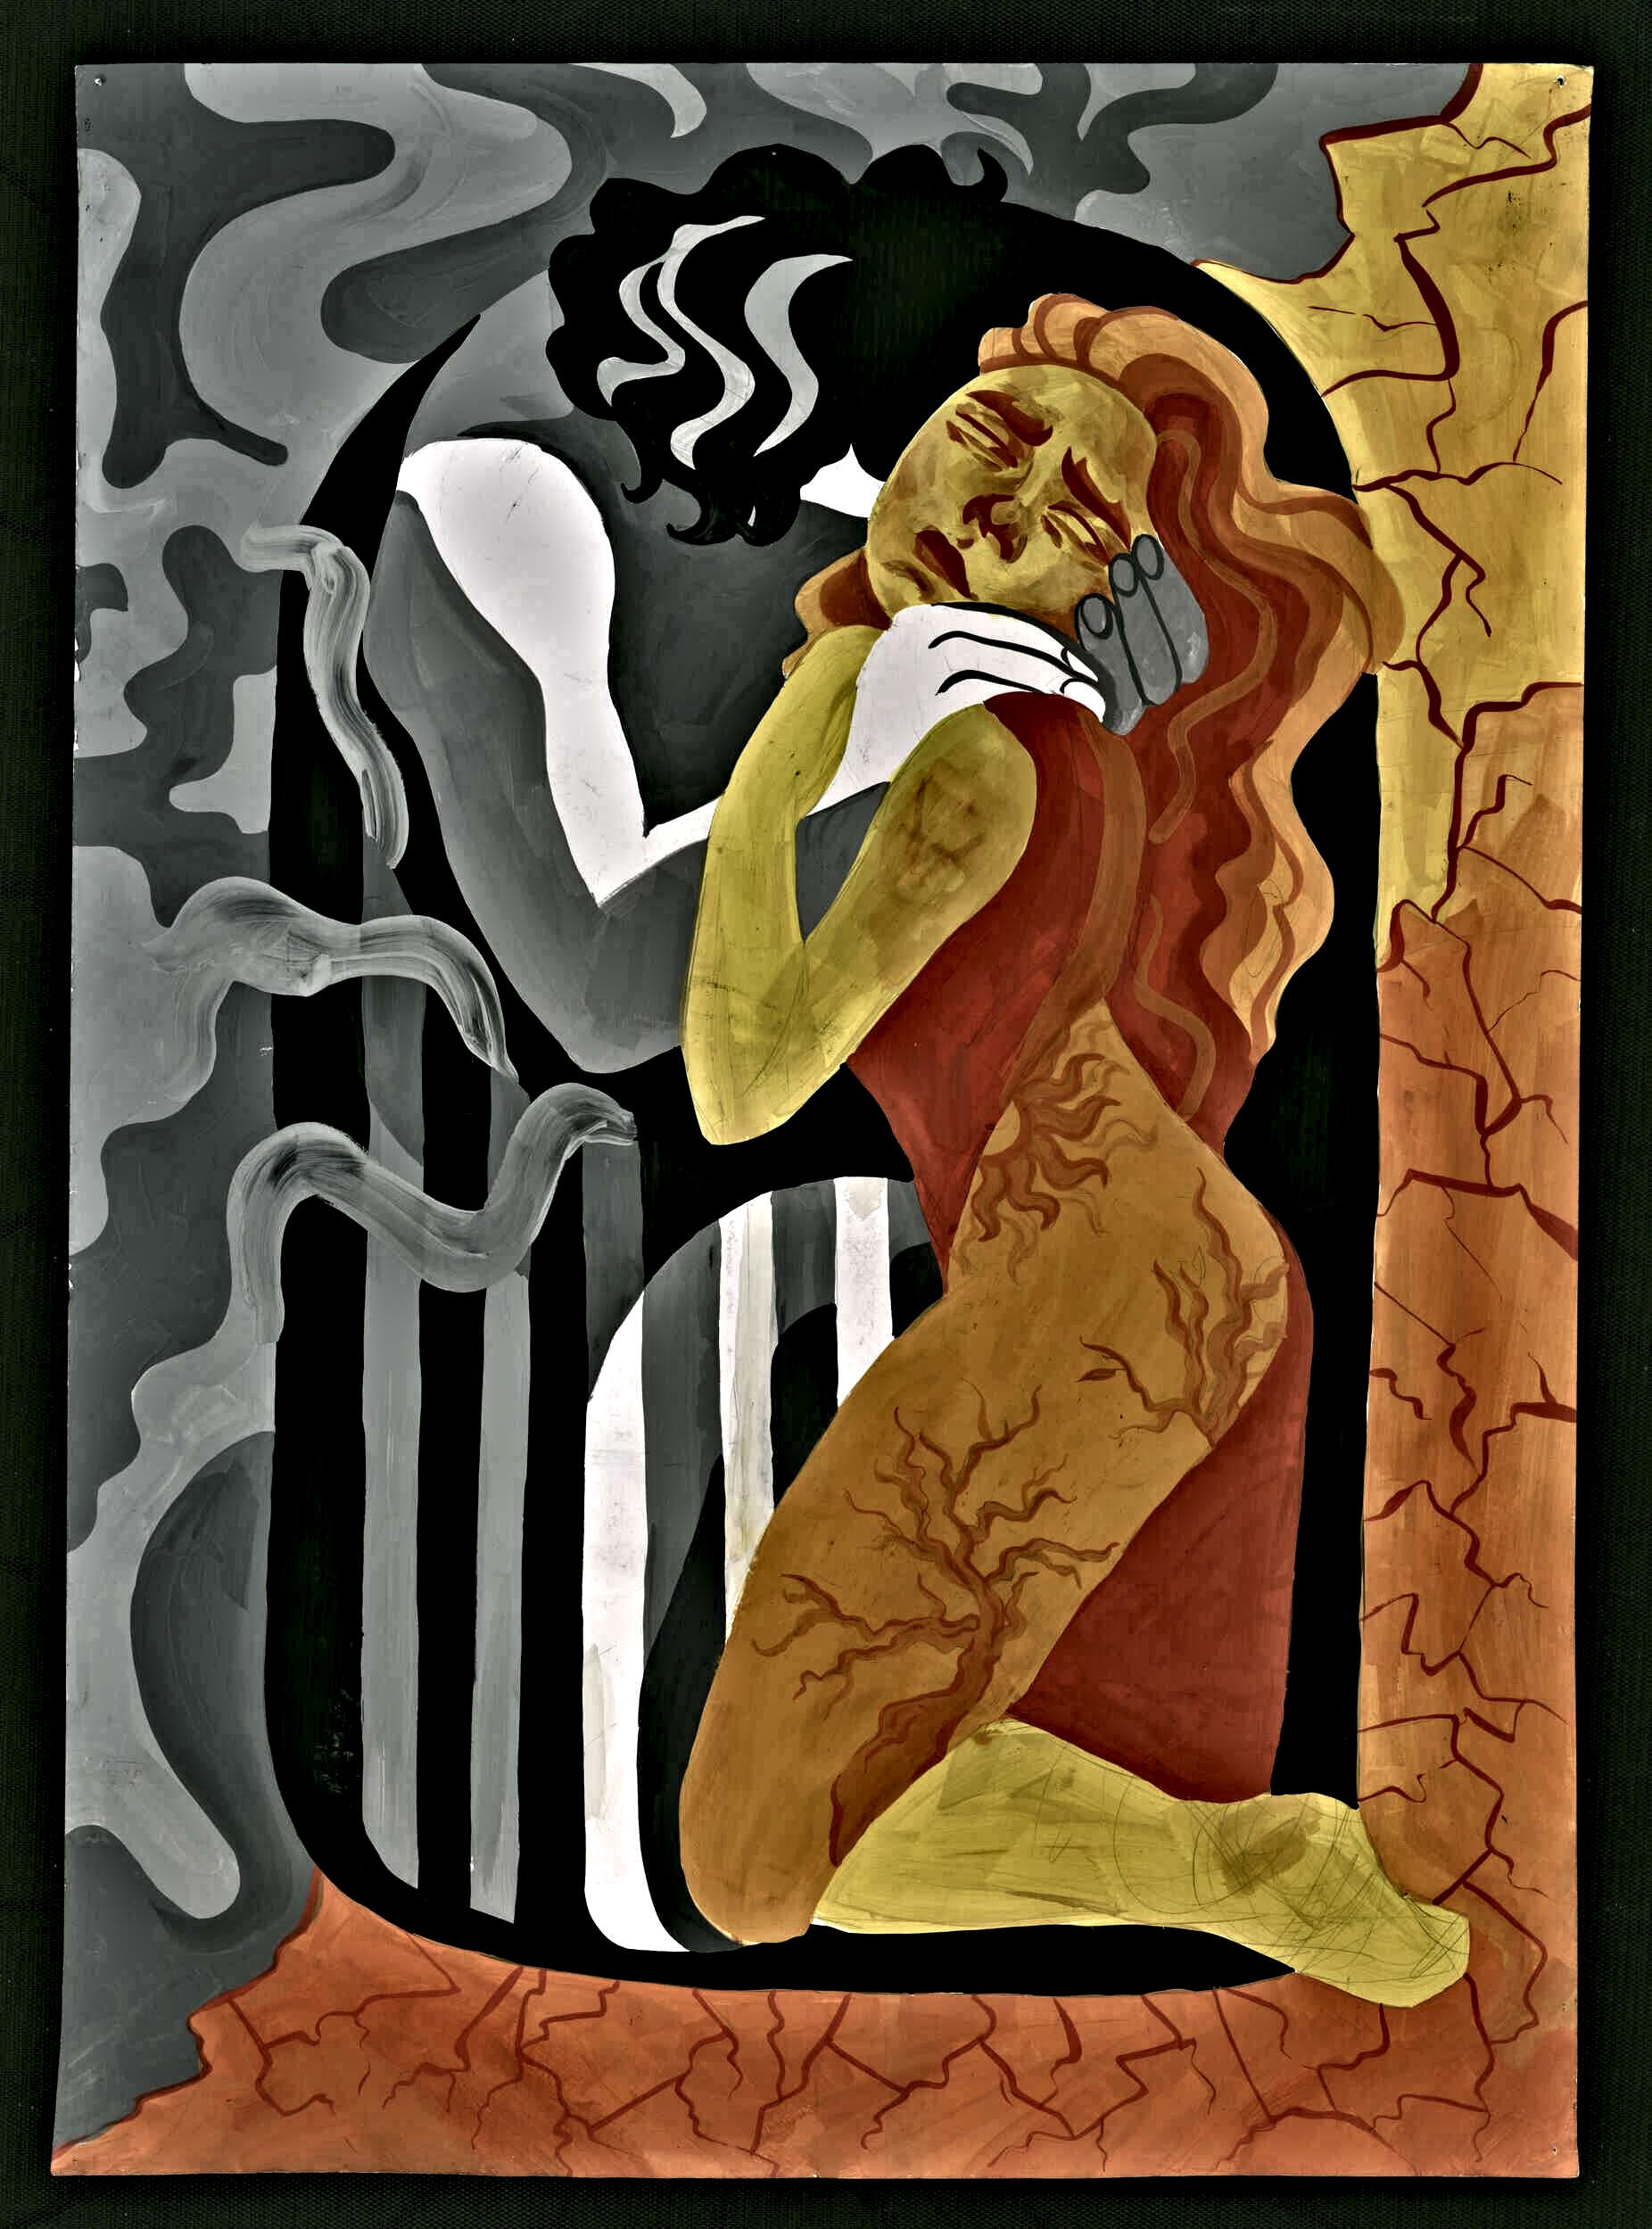
\includegraphics[width=0.45\textwidth]{images/style_augments/2020_14-17_2051_UKR_R_C_texture.jpg}
         \caption{}
     \end{subfigure}
     \hfil
     \begin{subfigure}[b]{0.5\textwidth}
         \centering
         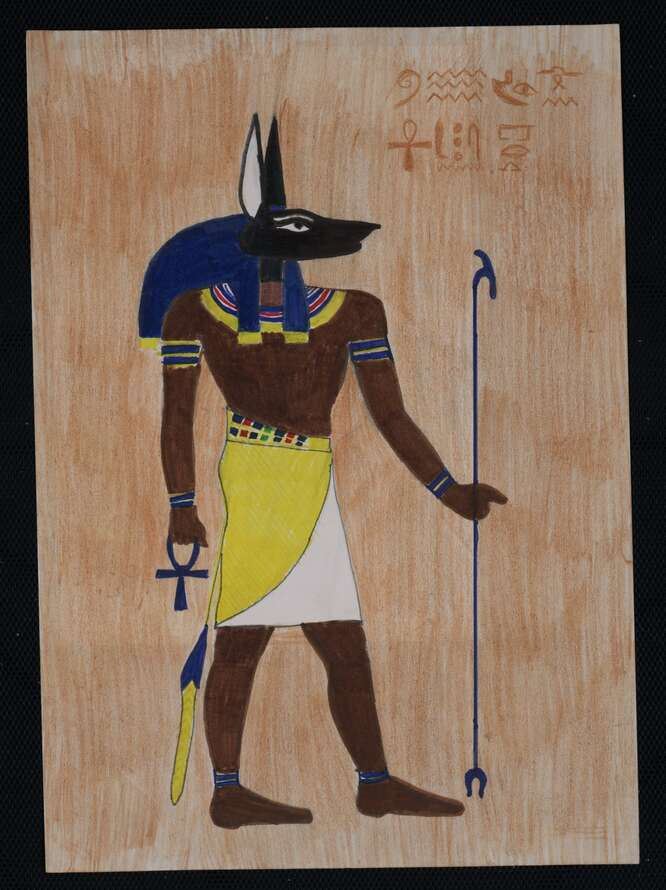
\includegraphics[width=0.45\textwidth]{images/style_augments/2019_14-17_0188_RUS_R_C.jpg}\hfil
         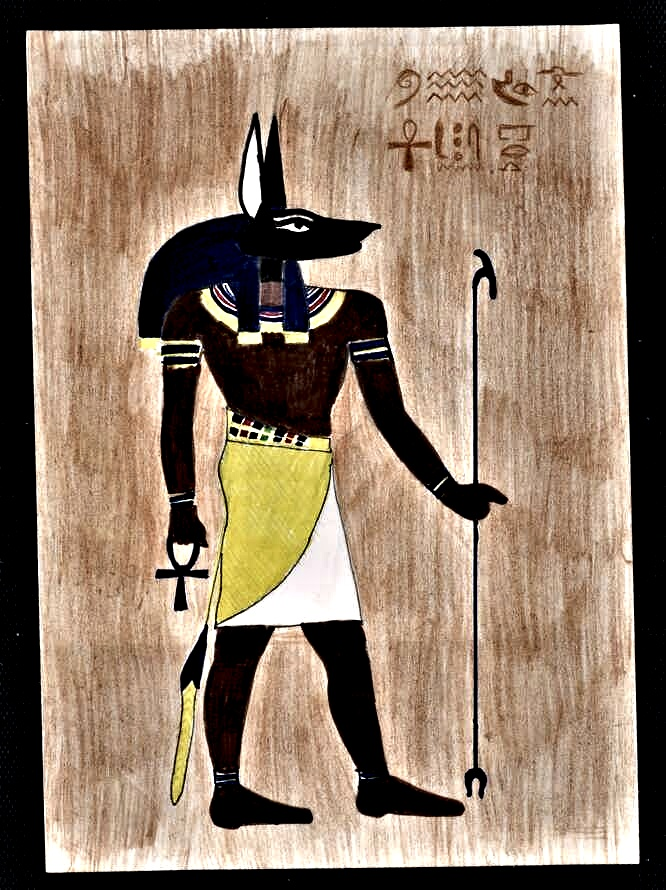
\includegraphics[width=0.45\textwidth]{images/style_augments/2019_14-17_0188_RUS_R_C_texture.jpg}
         \caption{}
     \end{subfigure}
     \caption{Examples of drawings (on left) after apply textured effect (on right)}
     \label{fig:texture-style-effects}
\end{figure}

\begin{figure}
     \centering
     \begin{subfigure}[b]{0.5\textwidth}
         \centering
         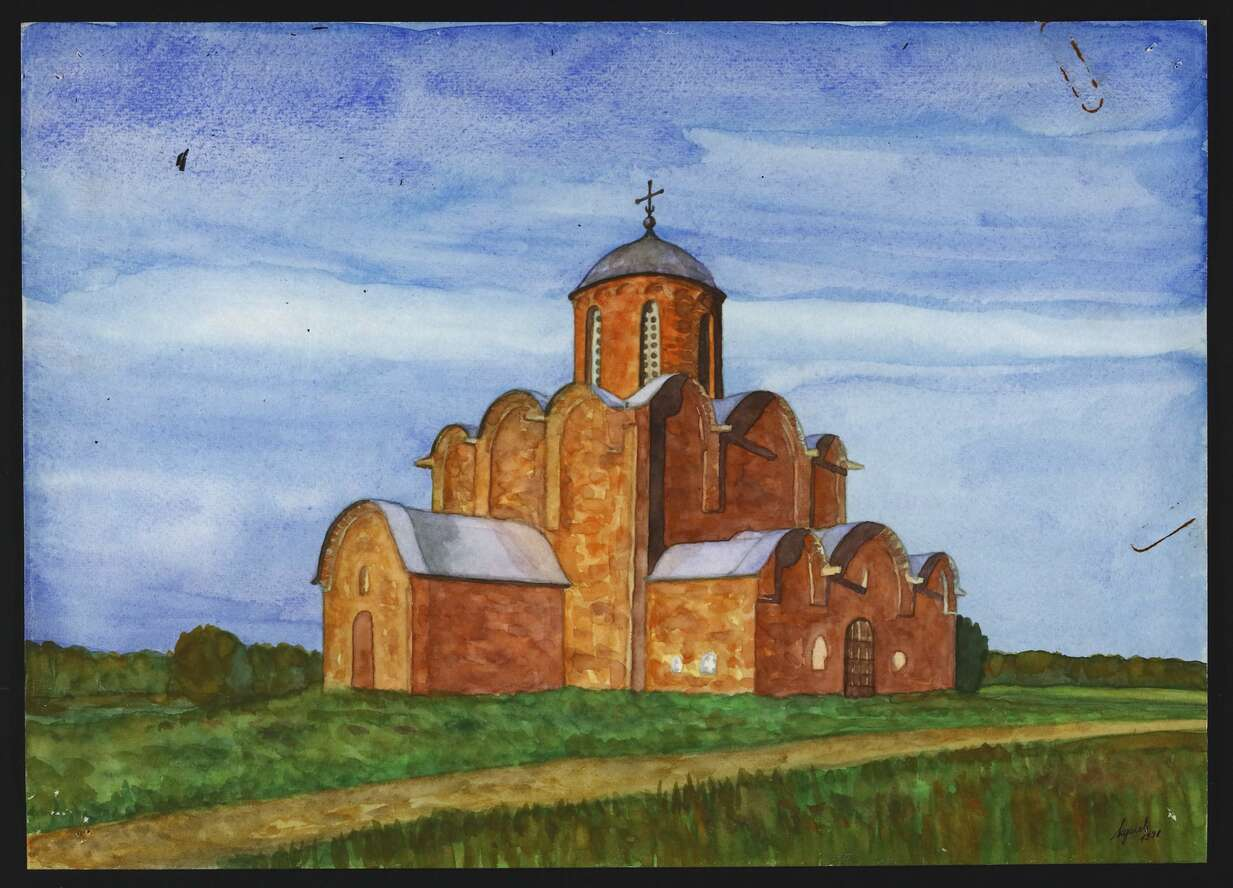
\includegraphics[width=0.45\textwidth]{images/style_augments/1998_14-17_0101_RUS_R_C.jpg}\hfil
         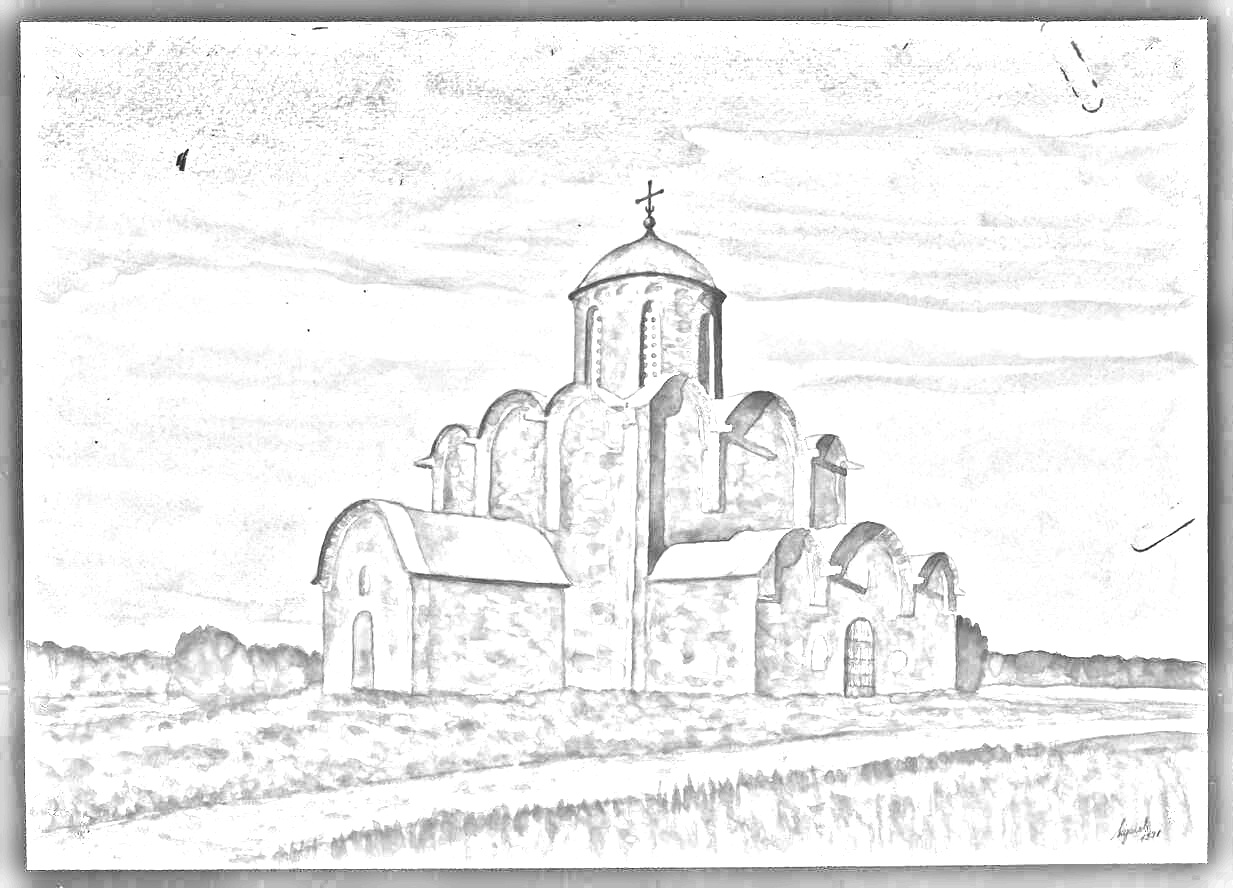
\includegraphics[width=0.45\textwidth]{images/style_augments/1998_14-17_0101_RUS_R_C_pencil_gray.jpg}
         \caption{}
     \end{subfigure}
     \hfil
     \begin{subfigure}[b]{0.5\textwidth}
         \centering
         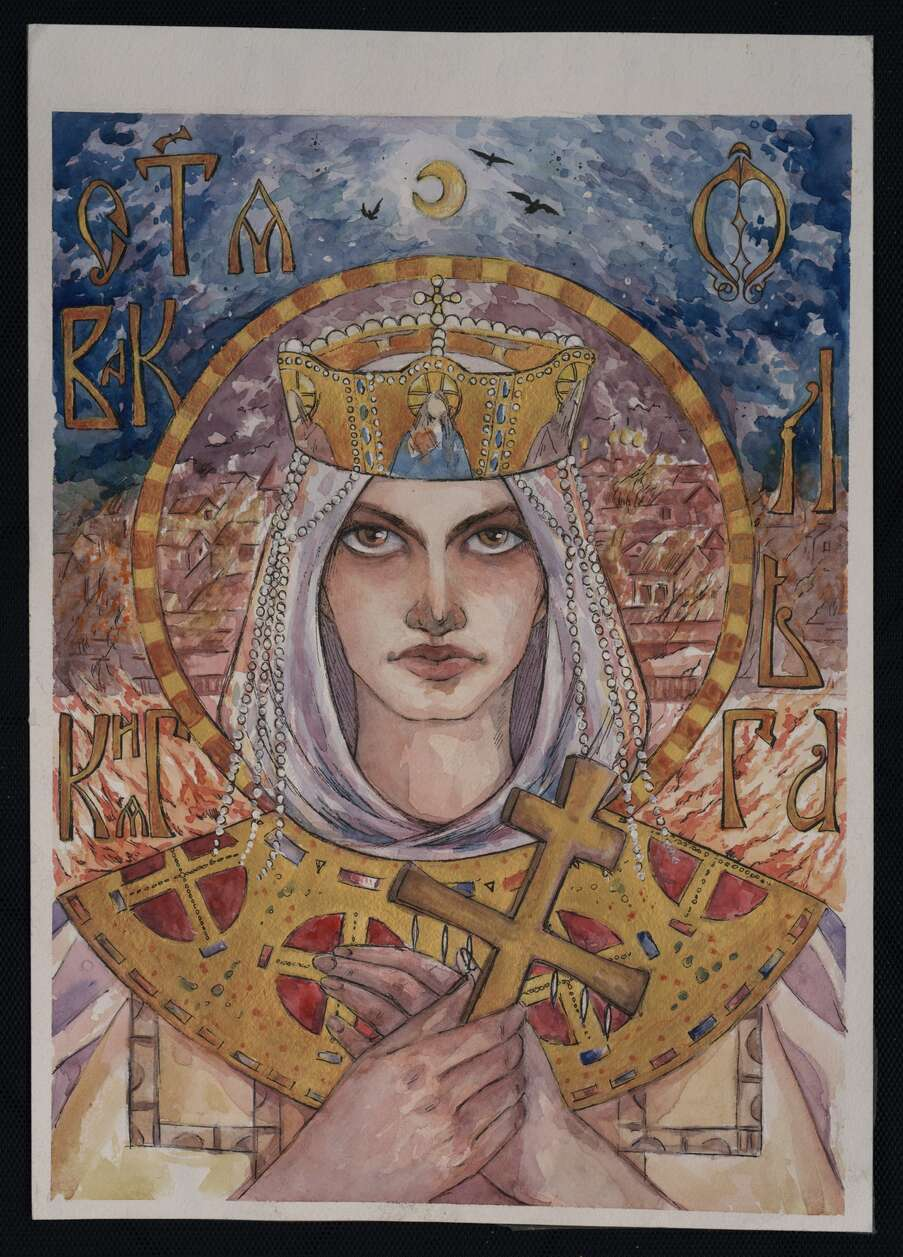
\includegraphics[width=0.45\textwidth]{images/style_augments/2019_14-17_0193_RUS_R_C.jpg}\hfil
         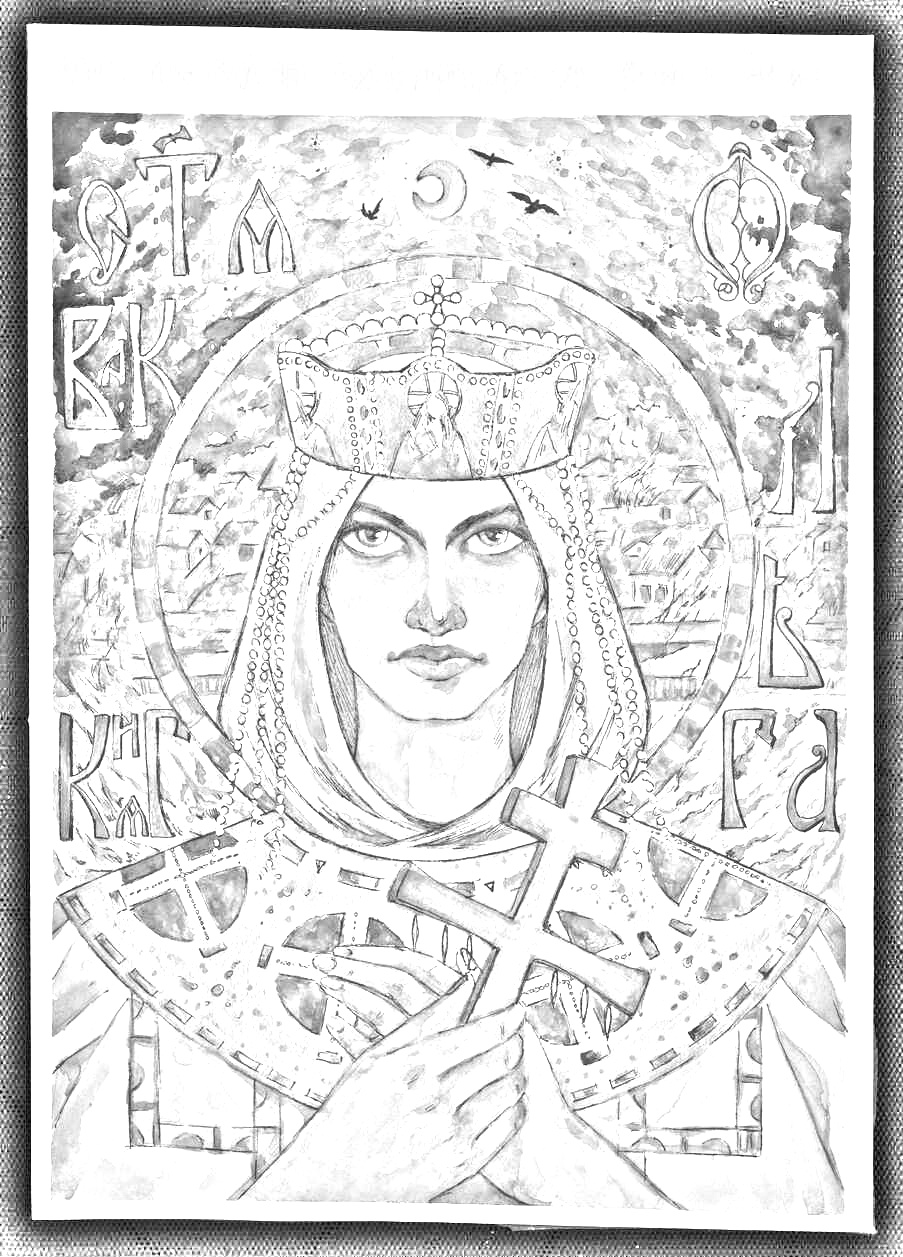
\includegraphics[width=0.45\textwidth]{images/style_augments/2019_14-17_0193_RUS_R_C_pencil_gray.jpg}
         \caption{}
     \end{subfigure}
     \hfil
     \begin{subfigure}[b]{0.5\textwidth}
         \centering
         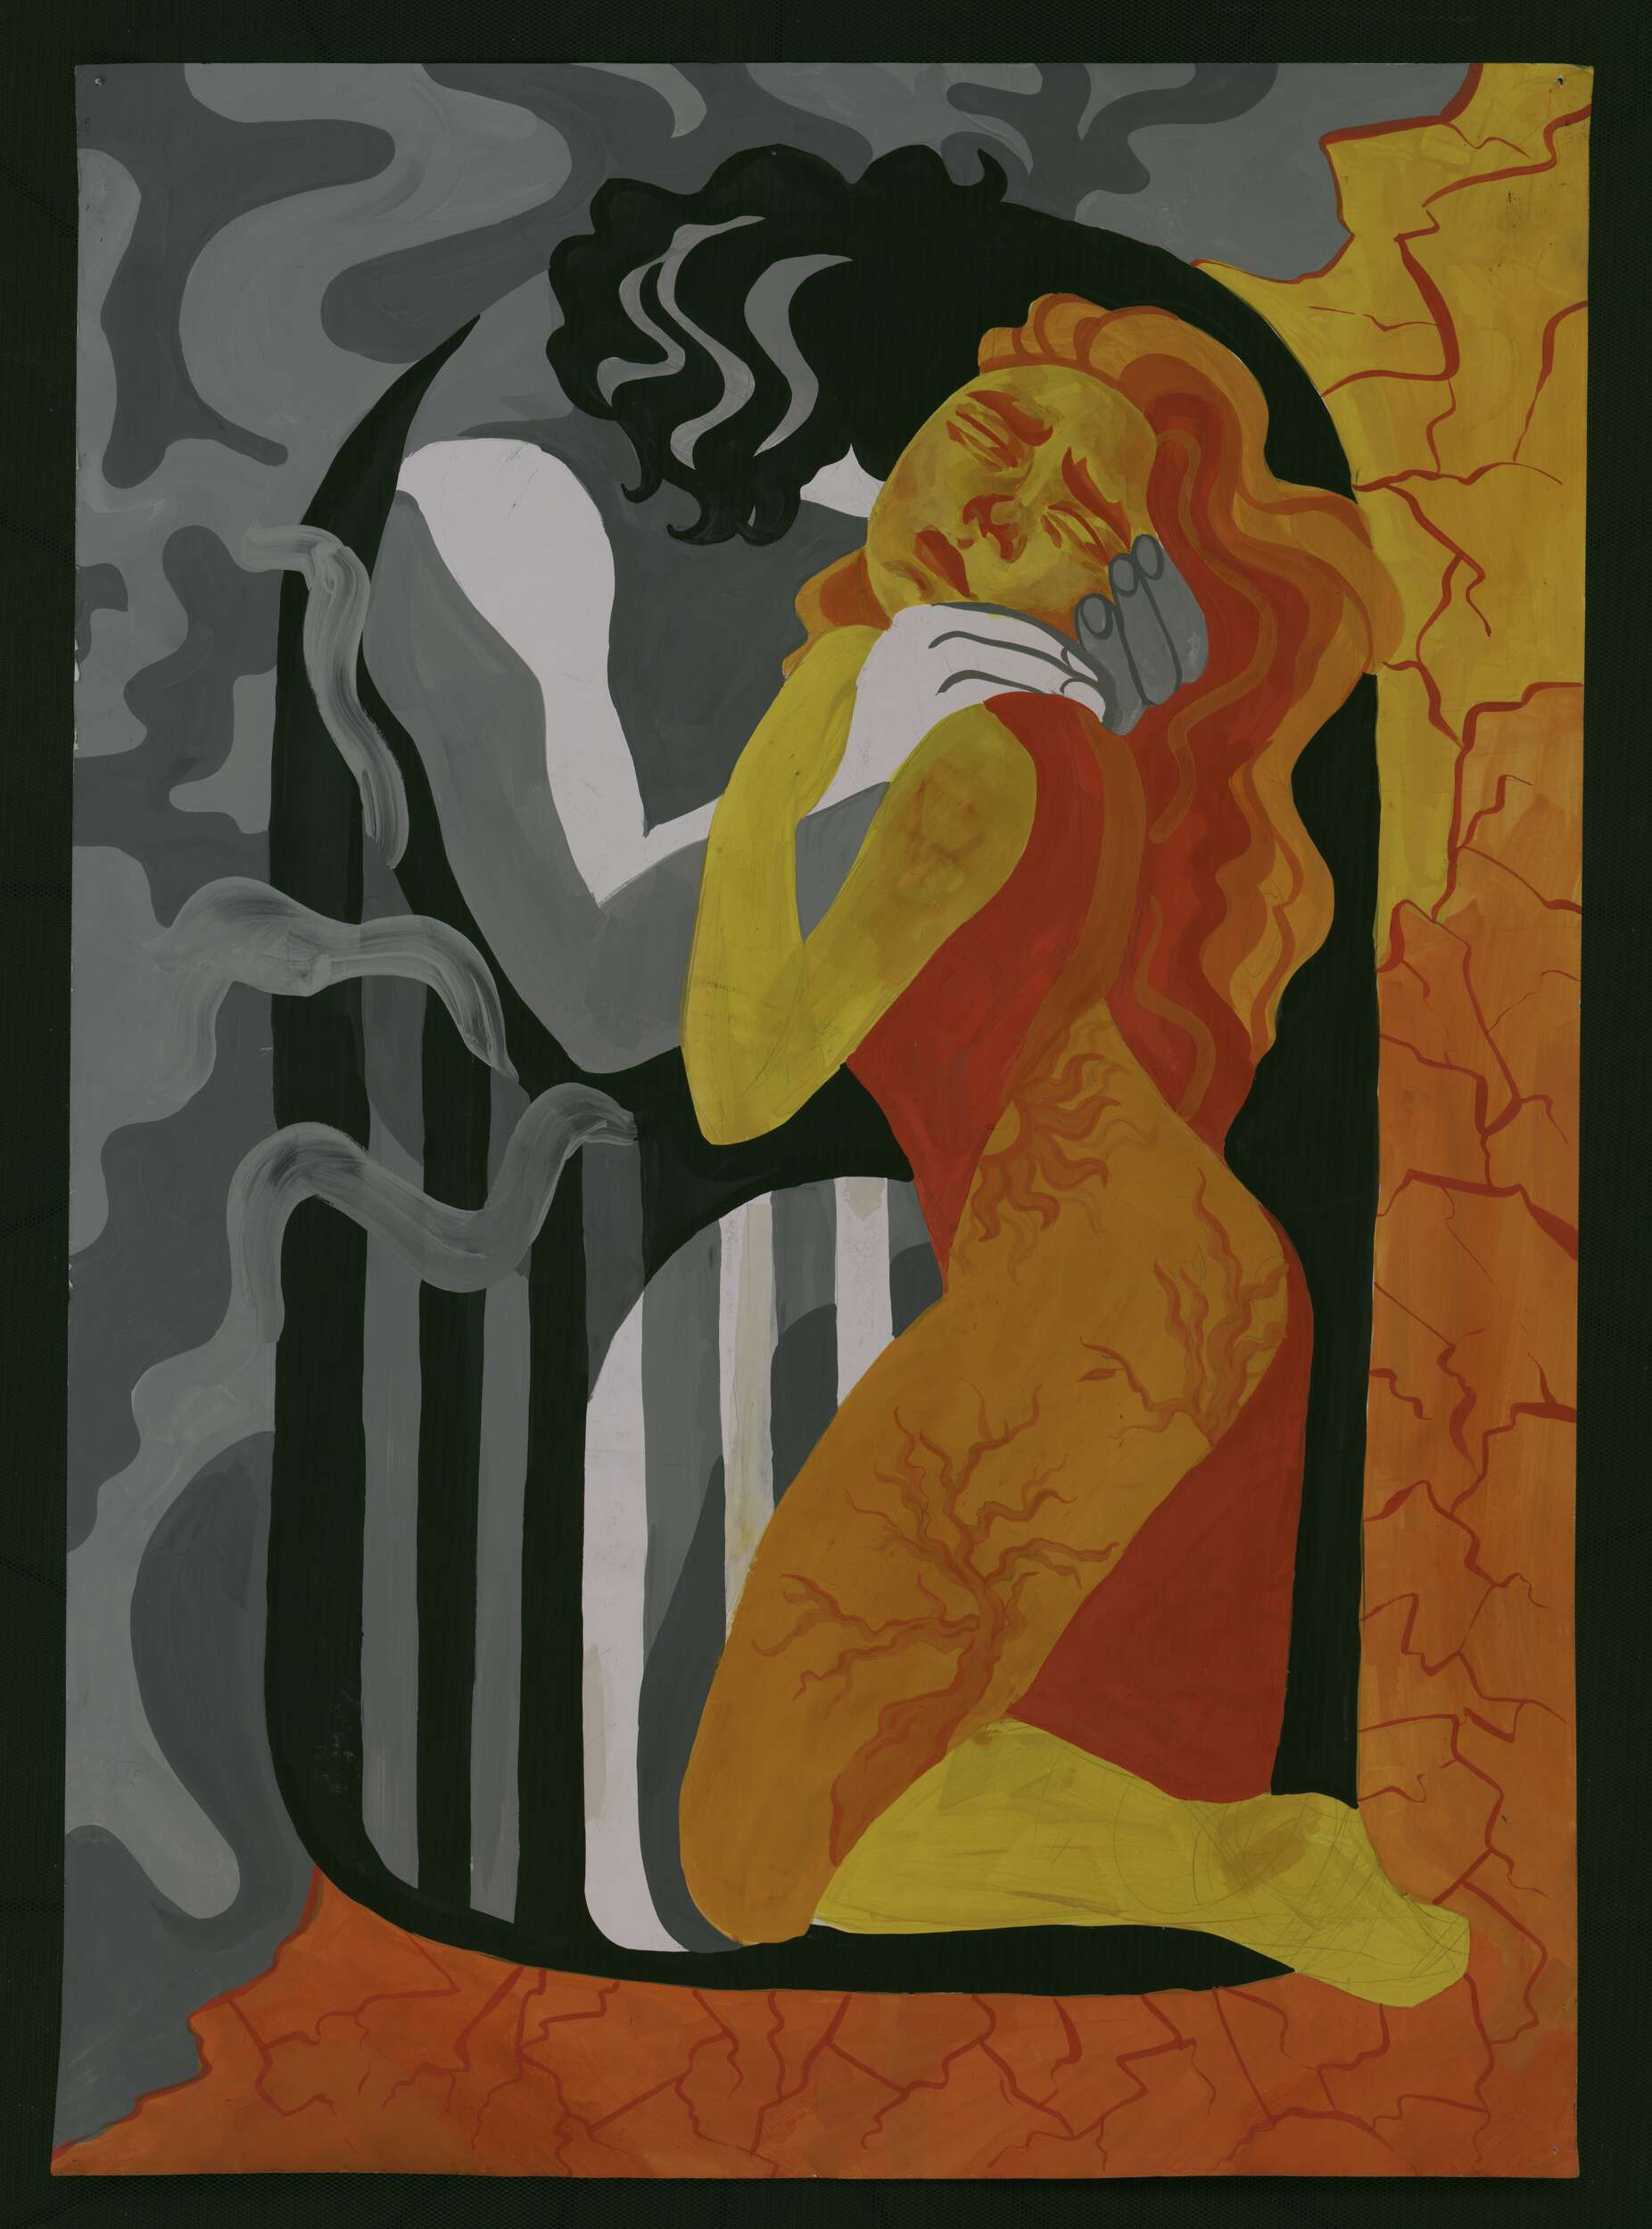
\includegraphics[width=0.45\textwidth]{images/style_augments/2020_14-17_2051_UKR_R_C.jpg}\hfil
         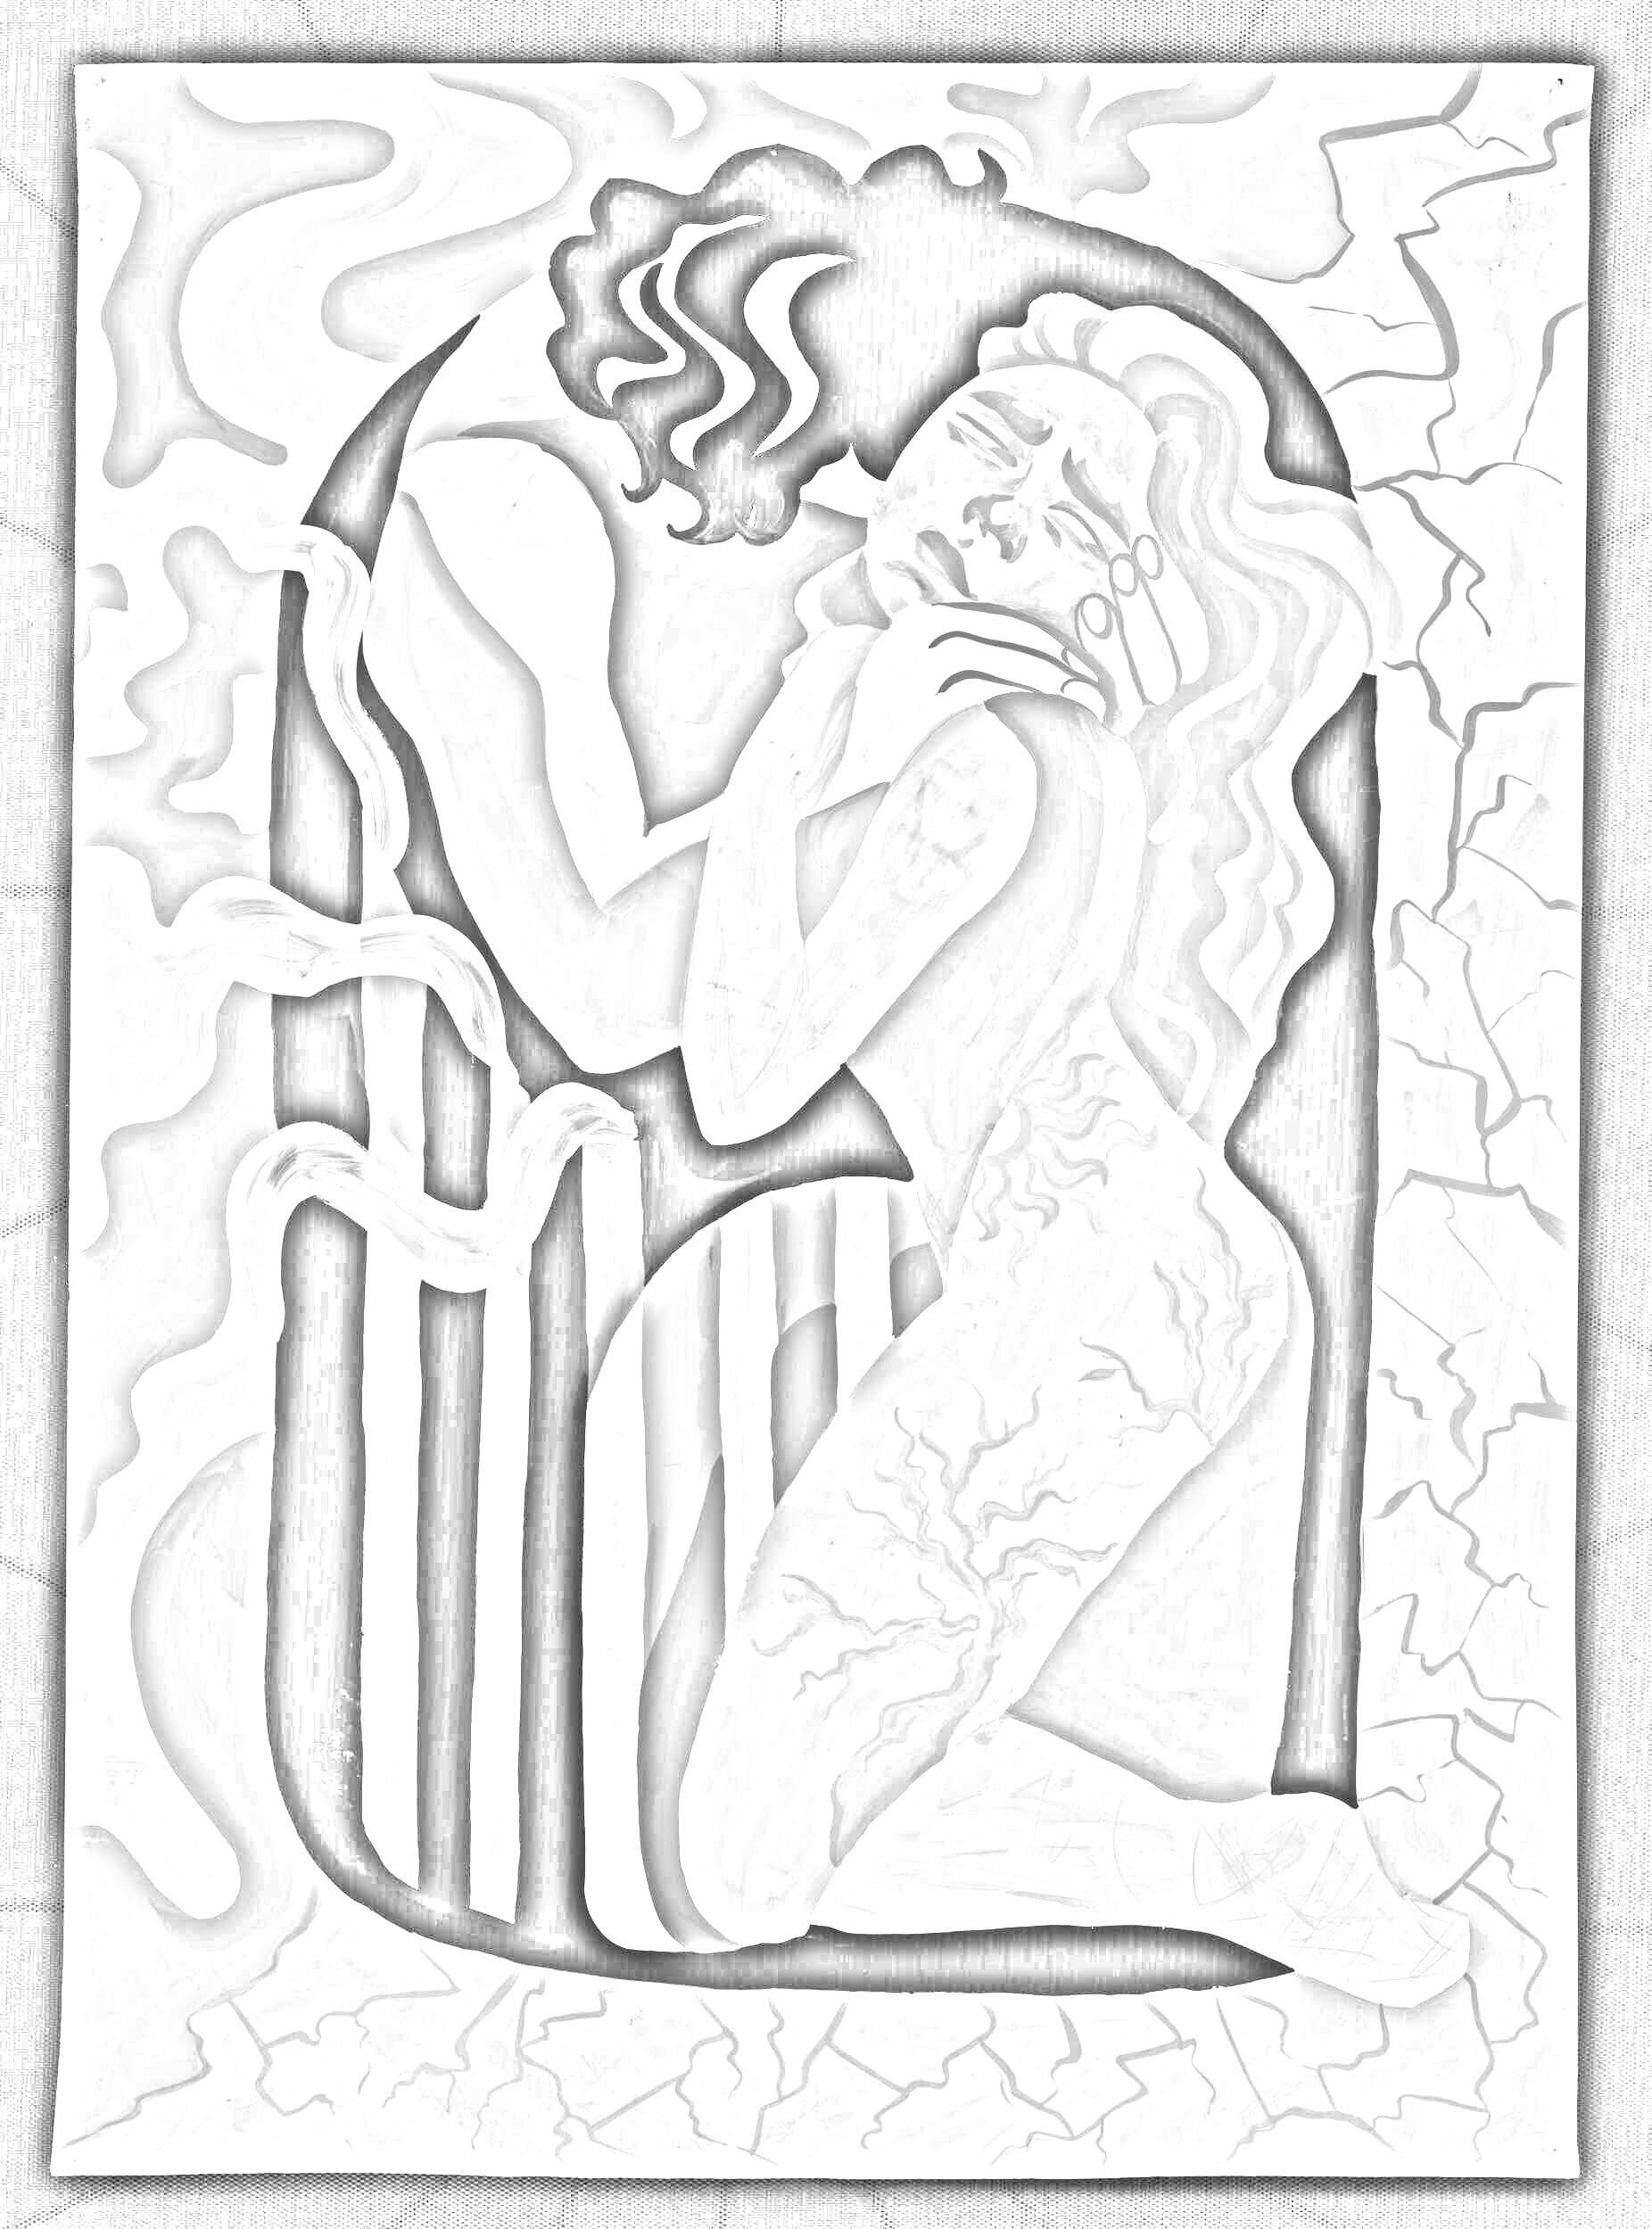
\includegraphics[width=0.45\textwidth]{images/style_augments/2020_14-17_2051_UKR_R_C_pencil_gray.jpg}
         \caption{}
     \end{subfigure}
     \hfil
     \begin{subfigure}[b]{0.5\textwidth}
         \centering
         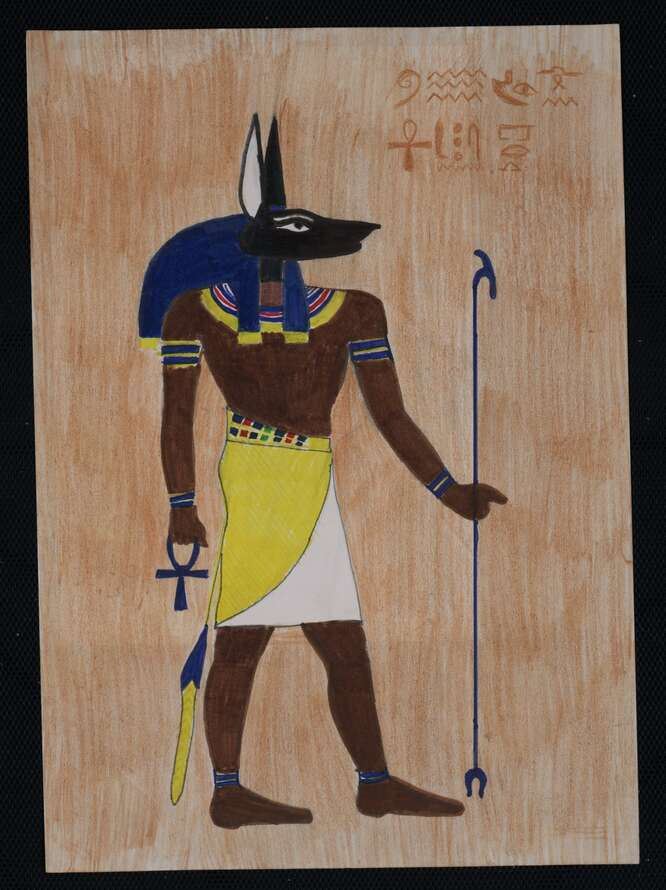
\includegraphics[width=0.45\textwidth]{images/style_augments/2019_14-17_0188_RUS_R_C.jpg}\hfil
         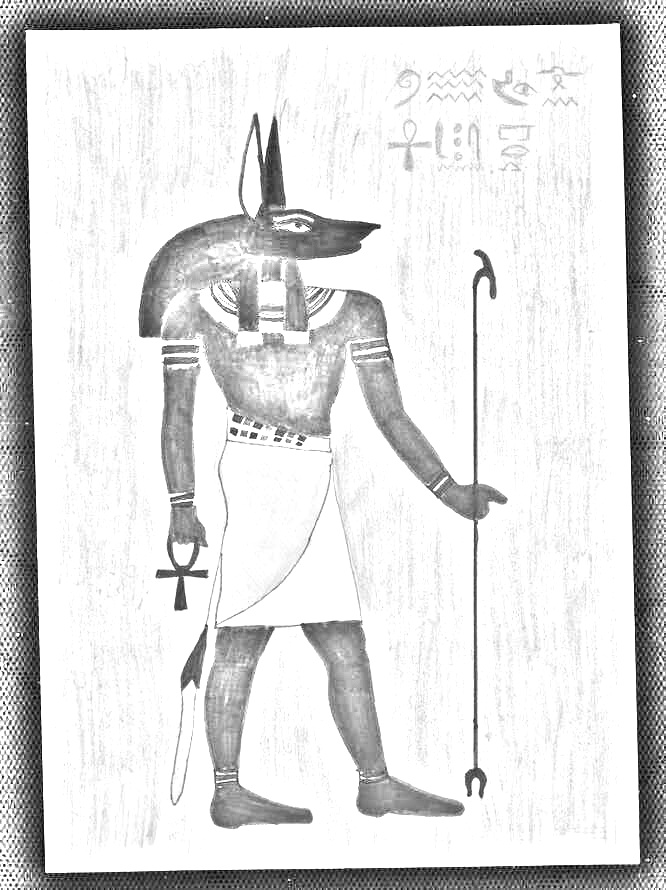
\includegraphics[width=0.45\textwidth]{images/style_augments/2019_14-17_0188_RUS_R_C_pencil_gray.jpg}
         \caption{}
     \end{subfigure}
     \caption{Examples of drawings (on left) after apply pencil sketch effect (on right)}
     \label{fig:pencil_gray-style-effects}
\end{figure}


\subsection{Style Augmentation}

As discussed in earlier chapters, the children do not necessarily recreate the famous artworks using the same material and technique. Therefore, augmenting the drawings in the training set helps to consider the diversity to some extent. This augmentation step was performed offline in addition to the preprocessing or transformations mentioned above. The training drawings were expanded with five styles using the effects available in the OpenCV library, increasing the training dataset \begin{math} 6 \end{math} times.
\subsubsection{Oil Painting}

An oil painting effect was applied using the OpenCV's \textit{oilPainting} function in the \textit{xphoto} module by setting \textit{size} and \textit{dynRatio} parameters to \begin{math} 7 \end{math} and \begin{math} 1 \end{math}, respectively. Figure \ref{fig:oil-style-effects} shows the result of converting some drawings.

\subsubsection{Water Color}

OpenCV's stylization function applies the watercolor effect to the image with \textit{sigma\_s} set to \begin{math} 60 \end{math} and \textit{sigma\_r} as \begin{math} 0.6 \end{math}. \textit{sigma\_s} controls the size of the neighborhood, and \textit{sigma\_r} controls averaging of colors in the chosen neighborhood. The drawings with the watercolor effect are shown in Figure \ref{fig:water-style-effects}.

\subsubsection{Textured}

The drawings were converted into textured sketches (Figure \ref{fig:texture-style-effects}) using the \textit{detailEnhance} function in OpenCV with \textit{sigma\_s} as \begin{math} 60 \end{math} and \textit{sigma\_r} as \begin{math} 0.4 \end{math}.

\subsubsection{Grayscale}
The grayscaled versions of the drawings obtained through OpenCV's standard \textit{cvtColor} function were also part of the training.

\subsubsection{Pencil Sketch}

A pencil sketch effect was applied to the drawings using a set of custom operations:
\begin{enumerate}
    \item Invert the grayscaled version of the image to reverse its colors.
    \item Apply a gaussian blur to the inverted image to reduce the noise and detail.
    \item Blend the grayscale and blurred images by dividing the former with the latter.
\end{enumerate}
The examples of drawings after applying this effect are shown in Figure \ref{fig:pencil_gray-style-effects}.

% \section{Evaluation}

% The models are compared and evaluated using Mean Position (MP), Recall (R), and Mean Average Precision (MAP) metrics. In line with the discussion in Section \ref{chap:4:sec:metrics-descrp:recall}, the Recall@k (R@k) using the top 20 (R@20), 50 (R@50), 100 (R@100), 200 (R@200), and 400 (R@400) retrieved artworks are compared. The performance of the model at these different positions conveys its robustness.

\section{Pre-trained Models - Baseline solution}

\begin{table}[ht]
    \centering
    \begin{tabular}{c|c}
    \hline \hline
        Model & Baseline (ResNeXT-101) \\ \hline \hline
        \textit{MP} & 1039.94 ± 178.51 \\
        \textit{MAP} & 12.5 ± 4.48 \\ 
        \textit{R@400} & 40.35 ± 3.63 \\
        \textit{R@200} & 32.98 ± 7.06 \\
        \textit{R@100} & 26.07 ± 7.51 \\
        \textit{R@50} & 23.53 ± 7.41 \\
        \textit{R@20} & 17.45 ± 6.1 \\ 
    \end{tabular}
    \caption{Metrics on the pre-trained ResNeXt-101 model}
    \label{tab:baseline-metrics}
\end{table}

The CNN models trained on image classification act as baseline models, and Table \ref{tab:baseline-metrics} shows the results of drawing-artwork pattern matching using a pre-trained ResNeXt-101 architecture. For nearly 60\% of drawings, the corresponding artwork does not appear in the top 400 results, and only for less than 20\% of drawings, the match is found in the first 20 ranked artworks. The mean appearance position of 1039 and the 12\% MAP suggests that the model has trouble finding the matching artwork and ranking it at the top. These results indicate room for improvement.

\section{Fine Tuning Experiments}

Training a Neural network requires adjusting various parameters and conditions. This section presents the results of experimentation in fine-tuning the model using style augmented images in the training dataset, followed by experiments using CNNs other than pre-trained models as the starting point.

\subsection{Style Augmentation}\label{chap:5:sec:stle-aug}

This experiment determines whether the presence of style-transferred drawings in the training data improves the model performance in identifying the matching artworks. Figure \ref{fig:baseline-ft-map} compares the distribution of the Mean Position (MP) of the retrieved artworks, and Table \ref{tab:aug-comp} provides the MAP and Recall measures. Baseline refers to the pre-trained ResNeXt-101 model, whereas FT Aug and FT No-Aug are the fine-tuned ResNeXt-101 models with and without using the style augmented drawings. The MPs in the fine-tuned models are always lower compared to the baseline. On average, the artworks appear 620 and 655 spots earlier in the FT No-Aug and FT Aug models.

\begin{figure}[ht]
\centering
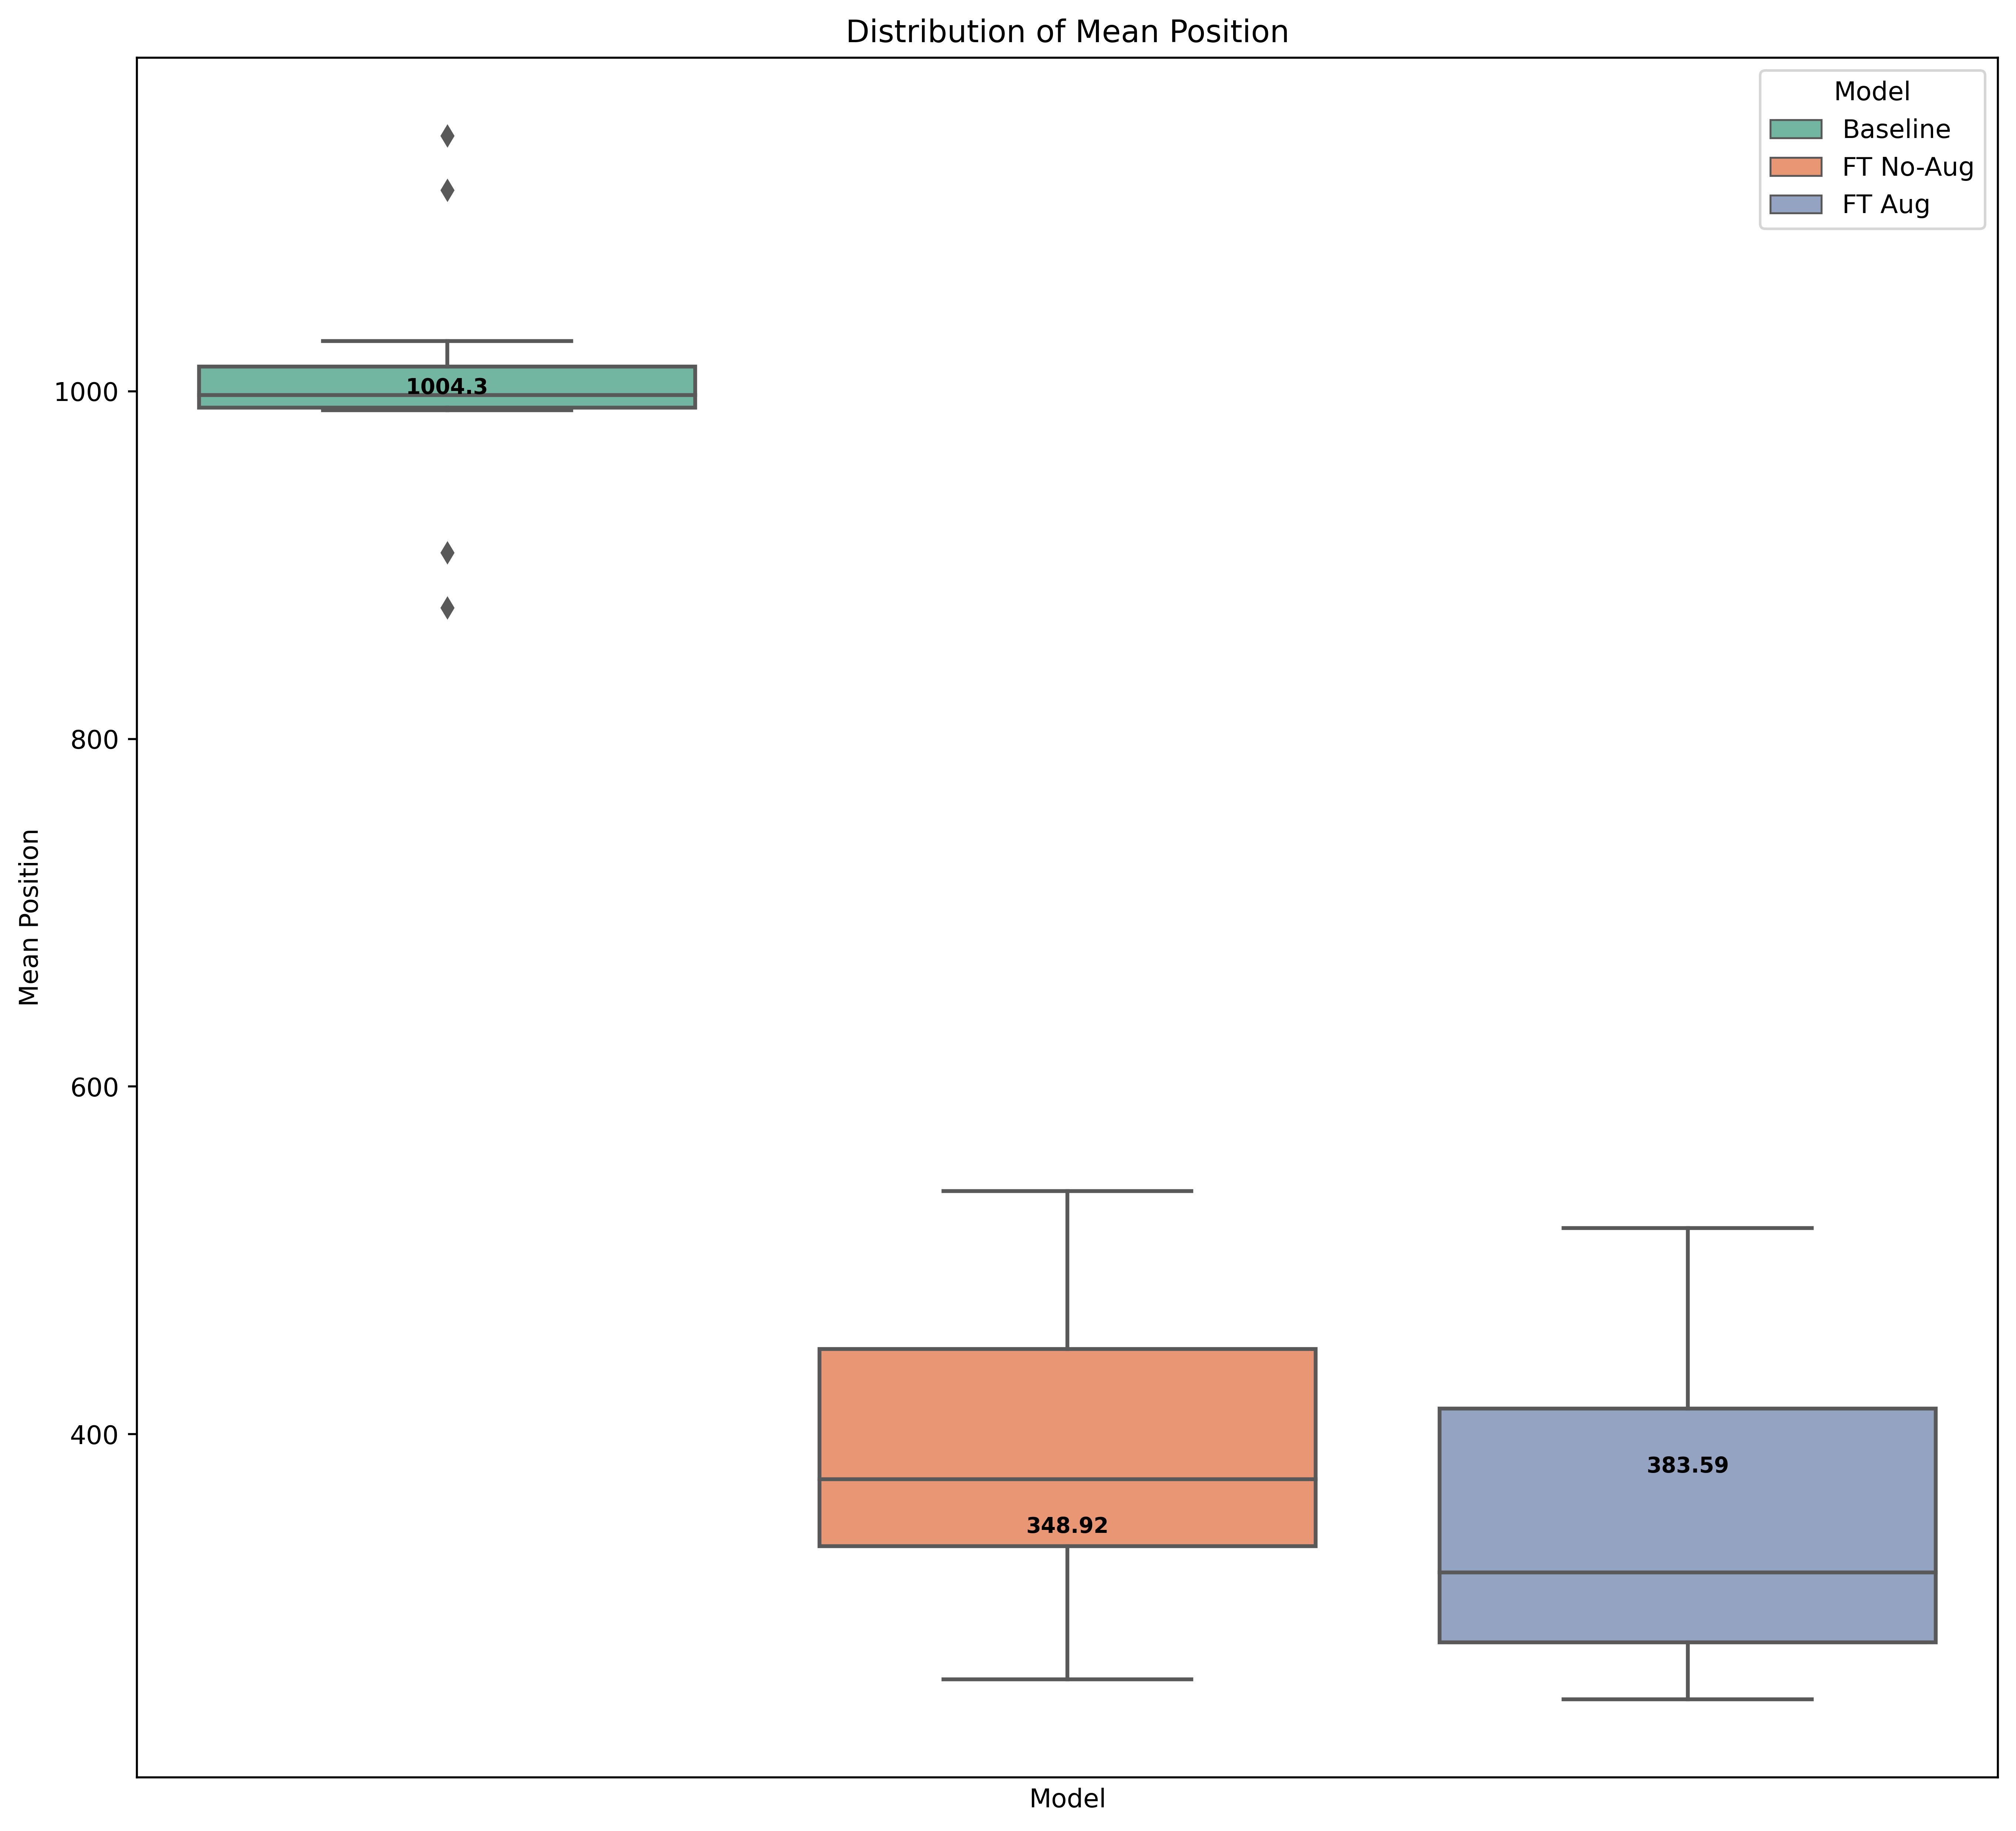
\includegraphics[width=\textwidth]{images/metrics/mp_baseline_500dpi.png}
  \caption{Mean Position comparison fine-tuning models using style augmented drawings}
  \label{fig:baseline-ft-map}
\end{figure}

\begin{table}[ht]
    \centering
    \begin{tabular}{c||c|c|c}
    \hline
        Model & Baseline & FT No-Aug & FT Aug \\ \hline \hline
        \textit{MAP} & 12.5 ± 4.48 & 26.82 ± 7.24 & 31.9 ± 10.03 \\ 
        \textit{R@400} & 40.35 ± 3.63 & 79.69 ± 8.11 & 87.18 ± 5.28 \\
        \textit{R@200} & 32.98 ± 7.06 & 72.29 ± 5.87 & 78.95 ± 7.26 \\
        \textit{R@100} & 26.07 ± 7.51 & 64.42 ± 8.44 & 67.38 ± 6.38 \\
        \textit{R@50} & 23.53 ± 7.41 & 54.32 ± 8.26 & 57.11 ± 11.26 \\
        \textit{R@20} & 17.45 ± 6.1 & 	44.99 ± 9.02 & 50.43 ± 11.7 \\ 
    \end{tabular}
    \caption{Evaluation metrics of fine-tuning models using style augmented drawings}
    \label{tab:aug-comp}
\end{table}

The FT No-Aug model improves recall by \textit{39.34}, \textit{39.31}, \textit{38.35}, \textit{30.79}, and \textit{27.54} percentage points from R@400 to R@50 compared to the baseline. Similarly, the recall values in FT Aug improved by \textit{46.83}, \textit{45.97}, \textit{41.31}, \textit{33.58}, and \textit{32.98} percentage points. The model trained using the augmented drawings improves the retrieval performance significantly. While the FT No-Aug model also improves from baseline. However, analyzing the retrievals of FT No-Aug shows that the artworks in the training set populate the top ranks irrespective of the drawing, hinting at overfitting.

Therefore, fine-tuning the model with style-augmented drawings provides better performance without overfitting the training data than the model fine-tuned otherwise.

\subsection{Models trained for detection of pattern propagation}\label{chap:5:sec:ludo-models}

Transfer learning methods in deep computer vision usually refer to using a CNN trained for image classification data using ImageNet data for other tasks. However, there is no restriction on using models other than those trained on ImageNet. This subsection presents the results of evaluating the drawing-artwork retrieval problem with a model developed to find duplicate photographs of artworks.

Digitization of photo collections opens a window to perform a wide range of operations to process and extract information. In a photo collection of artworks, it is possible to have multiple photos of the same subject (painting, sculpture, carvings) either captured by the same person or a different one. Conversely, two paintings can have the same global composition with different local elements or vice versa, or they can be thematically related by depicting the same scene differently. Seguin \cite{Seguin2018MakingLA} developed a system (known as \textit{Replica}) to identify images sharing identical patterns in photos of artworks (Section \ref{chap:2:sec:REPLICA}). Ludovica \cite{Ludovica2022} expands this work further to cluster photographs of paintings sharing patterns where duplication or re-creation of a visual object with an inspiration amounts to pattern sharing irrespective of the factors causing it.

\afterpage{
    \clearpage
    % \thispagestyle{empty}
    \centering
    \begin{landscape}

        \begin{table}
                \begin{tabular}{|c||c|c|c|c|c|c|}
                    \hline
                    Model & {MAP} & {R@400} & {R@200} & {R@100} & {R@50} & {R@20} \\ \hline \hline
                    \textit{Baseline} & 12.5 ± 4.48 & 40.35 ± 3.63 & 32.98 ± 7.06 & 26.07 ± 7.51 & 23.53 ± 7.41 & 17.45 ± 6.1 \\ \hline
                    \textit{Mini-Replica} & 28.73 ± 11.77 & 70.99 ± 5.94 & 60.4 ± 9.88 & 51.47 ± 10.25 & 45.1 ± 13.32 & 39.34 ± 12.55 \\ \hline
                    \textit{FT No-Aug Mini-Replica} & 33.26 ± 11.05 & 84.89 ± 5.02 & 76.46 ± 7.44 & 67.93 ± 9.0 & 62.23 ± 9.71 & 53.87 ± 10.45 \\ \hline
                    \textit{FT Aug Mini-Replica} & \textbf{35.26 ± 11.83} & \textbf{86.51 ± 5.9} & \textbf{80.62 ± 8.1} & \textbf{74.11 ± 7.59} & \textbf{65.48 ± 8.24} & \textbf{55.08 ± 6.94} \\ \hline
                    \textit{Clus-Replica} & 27.35 ± 9.6 & 68.86 ± 6.24 & 61.6 ± 7.49 & 56.22 ± 7.23 & 50.81 ± 8.6 & 41.11 ± 11.4 \\ \hline
                    \textit{FT No-Aug Clus-Replica} & 31.42 ± 6.14 & 77.82 ± 5.91 & 71.17 ± 7.4 & 66.14 ± 7.94 & 58.91 ± 10.57 & 53.85 ± 6.5 \\ \hline
                    \textit{FT Aug Clus-Replica} & 30.63 ± 6.69 & 76.76 ± 4.71 & 70.75 ± 5.69 & 65.46 ± 5.46 & 58.55 ± 9.46 & 49.9 ± 10.36 \\ \hline
                \end{tabular}
            \captionof{table}{Evaluation metrics of Replica variants}
            \label{tab:replica-comp}
        \end{table}

    \end{landscape}
    \clearpage
}

\begin{figure}[ht]
    \centering
    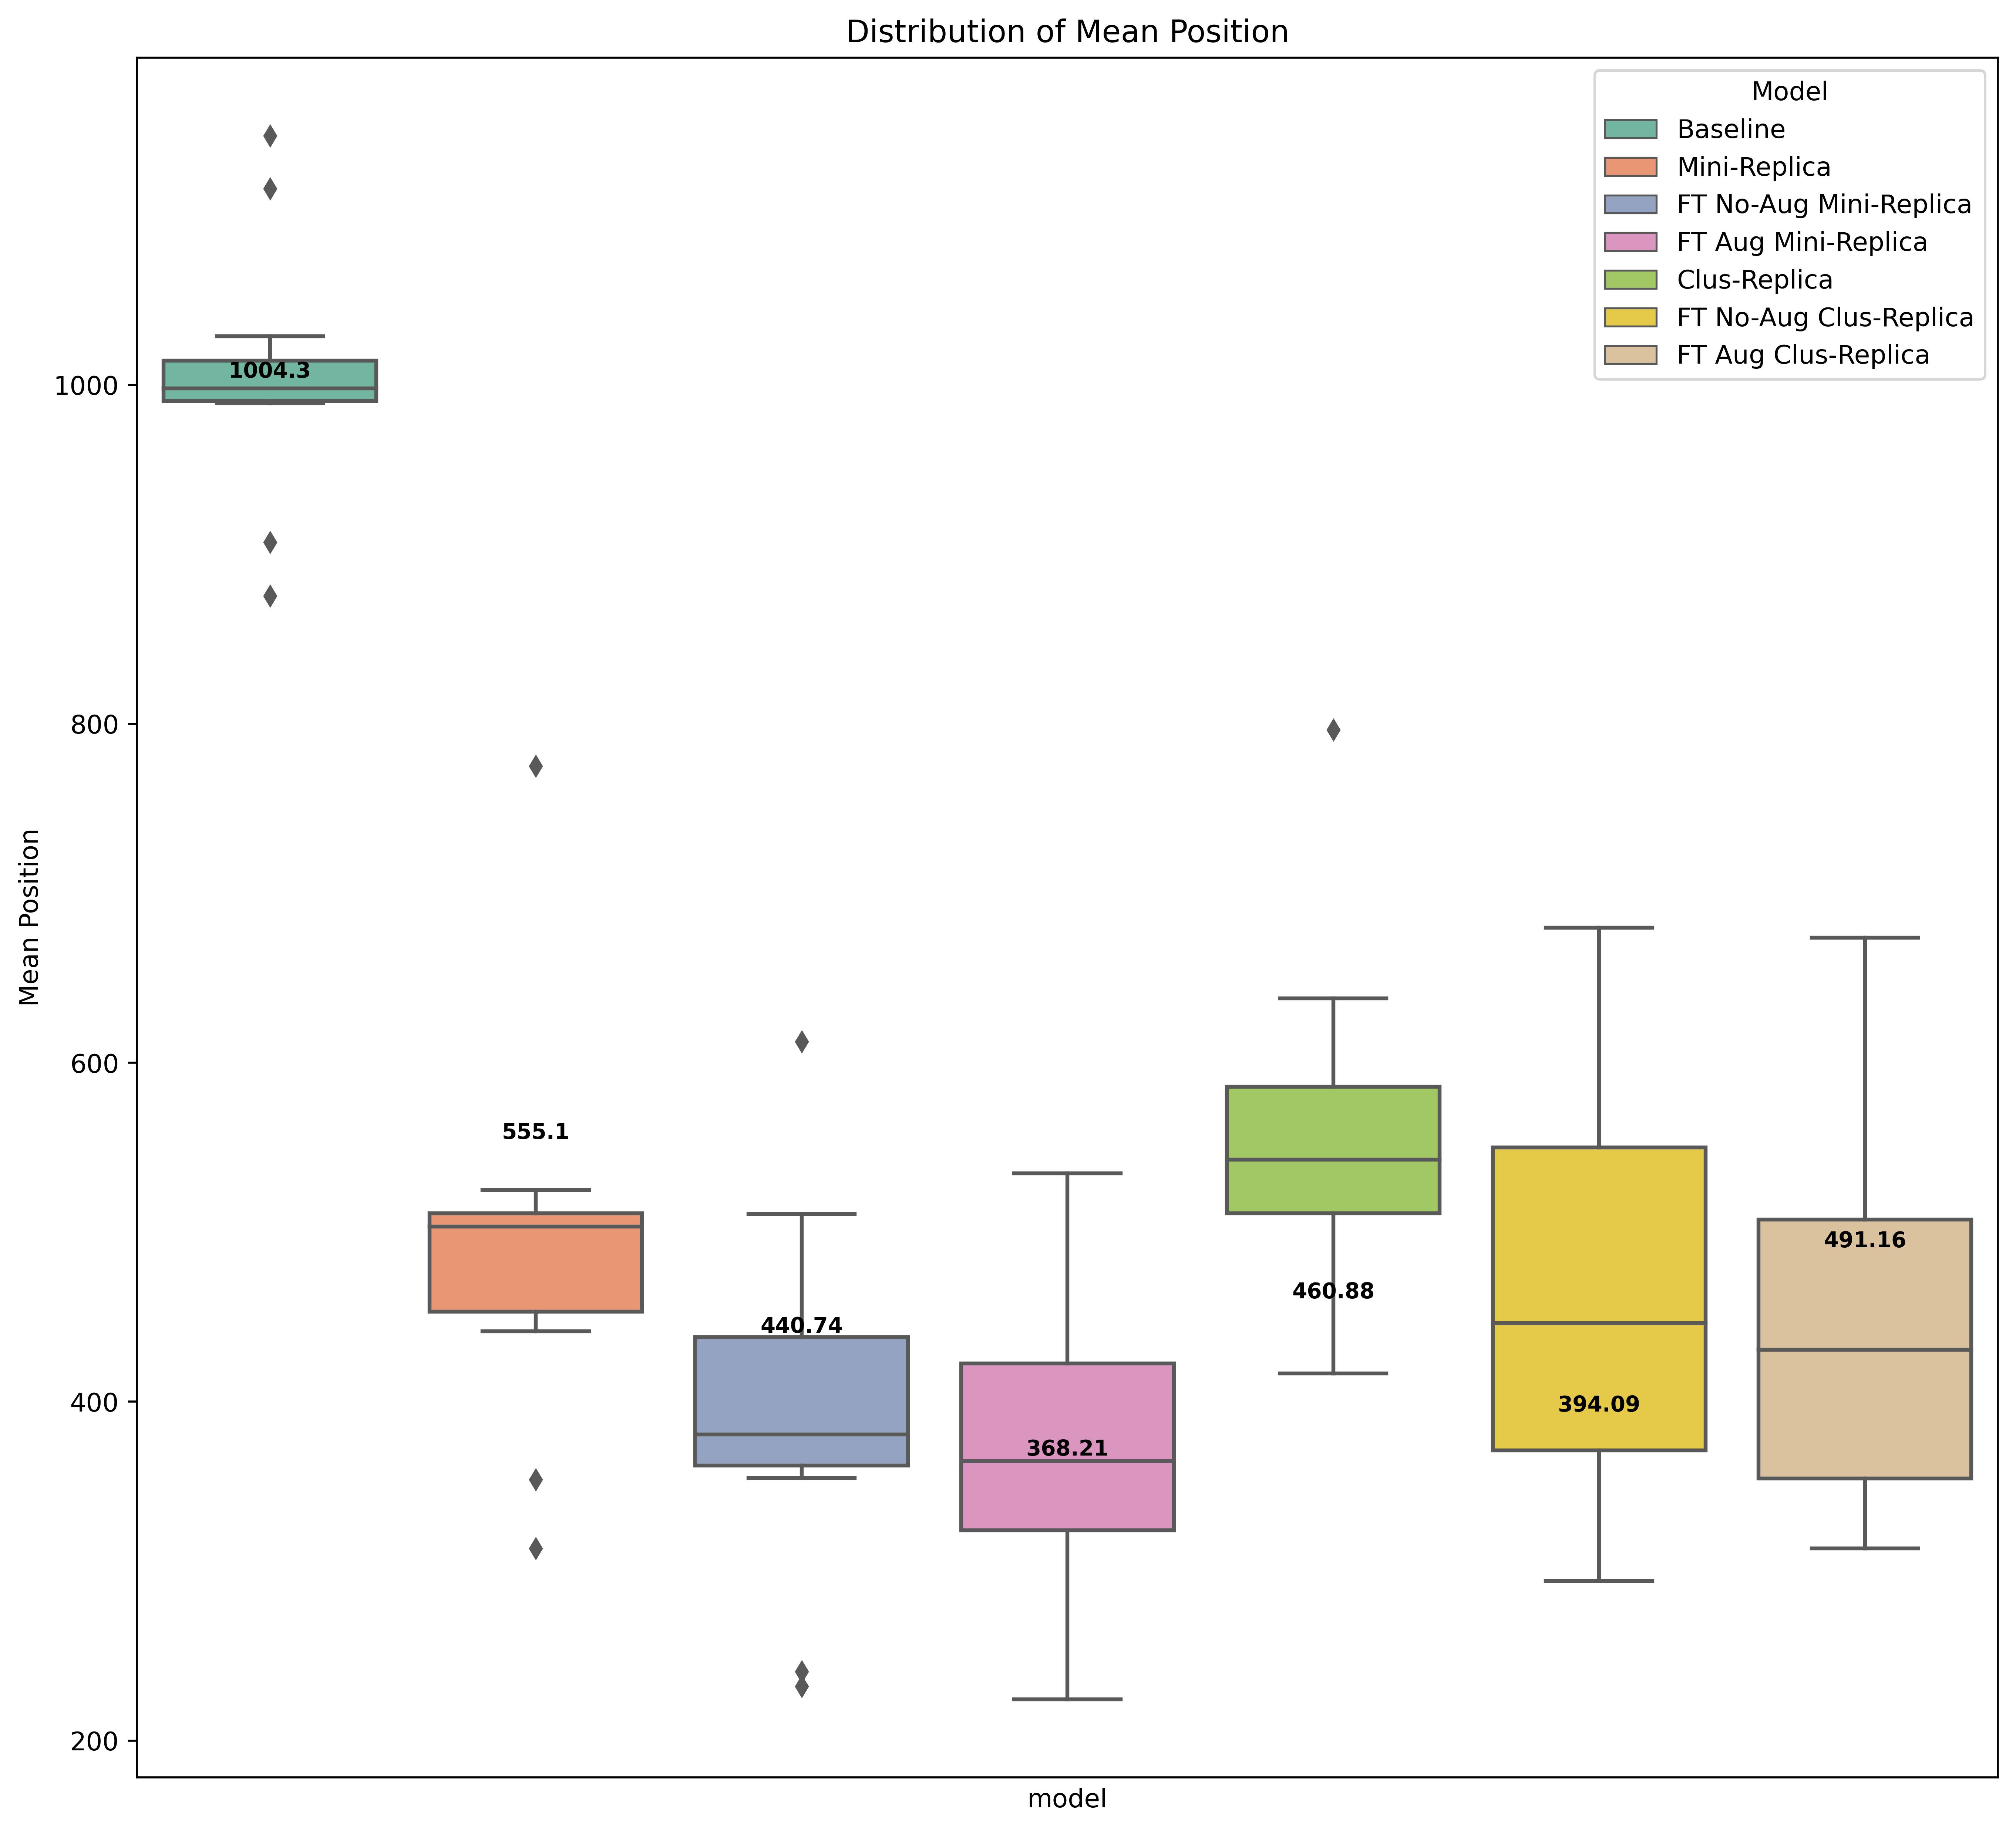
\includegraphics[width=\textwidth]{images/metrics/mp_replica_500dpi.png}
      \caption{Mean Position comparison of Evaluation metrics of Replica variants}
      \label{fig:replica-ft-mp}
\end{figure}

Two CNN models using ResNeXt-101 architecture made available by the extension form part of the experimentation in feature vector generation for the current drawing-artwork retrieval problem. The first model modernizes the Replica system through the latest CNN architecture to rank artwork photos based on their visual similarity. It is referred to as \textit{Mini-Replica} as it trains on a subset of data used in the original Replica project using triplet loss with cosine distance. The second model advances the Replica by clustering photos that share patterns. The training of the second model (\textit{Clus-Replica}) uses a modified triplet loss that includes the distance between the positive and negative sample of the triplet and an additional constraint to minimize the distance between the anchor and positive sample. This modified loss ensures that the distance between the anchor and positive samples is lower than between the anchor and negative, and the distance between positive and the anchor is lower than between the positive and negative samples. Additionally, it limits the distance between the anchor and positive sample to a maximal value. Apart from the loss function, the training data of Mini-Replica includes a mix of color and grayscale images, while Clus-Replica only uses grayscale images (8,900 images with 4,900 connections, i.e., annotated pairs sharing a visual pattern).

The experiments involving Mini-Replica and Clus-Replica are of two kinds:
\begin{itemize}
	\item First, retrieve and compare the artworks for the drawings using the feature vectors generated by the models trained on the Replica dataset.
	\item Second, fine-tune the models with the drawing-artwork pairs. As in Section \ref{chap:5:sec:stle-aug}, the experimentation involved the effect of style-augmented drawings in the dataset.
\end{itemize}

Table \ref{tab:replica-comp} and Figure \ref{fig:replica-ft-mp} show and visualize the evaluation metrics using the Replica variants compared with the baseline model (other nomenclature remains the same as before). Even before fine-tuning, the Mini-Replica and Clus-Replica models have lower mean positions and better recall than the pre-trained ResNeXt-101 model without fine-tuning. Furthermore, fine-tuning the model for the specific task boosts performance. The effect of augmented data is the same as earlier - training the model using the drawings alone overfits the train data. However, for the Clus-Replica model, training with the stylized drawings drops the model's ability to rank better.

\subsection{Models Comparision}\label{chap:5:sec:all-models}

\afterpage{
    \clearpage
    % \thispagestyle{empty}
    \begin{landscape}
    \centering
        \begin{table}
            \begin{tabular}{|c||c|c|c|c|c|c|}
                \hline
                Model & {MAP} & {R@400} & {R@200} & {R@100} & {R@50} & {R@20} \\ \hline
                \textit{Baseline} & 17.51 ± 6.39 & 47.29 ± 7.39 & 39.79 ± 7.26 & 35.08 ± 6.78 & 33.78 ± 7.35 & 27.13 ± 8.65 \\ \hline
                \textit{FT No-Aug} & 32.58 ± 8.86 & 82.46 ± 10.39 & 74.6 ± 10.77 & 66.9 ± 13.94 & 58.61 ± 14.83 & 51.99 ± 15.53 \\ \hline
                \textit{FT Aug} & 37.09 ± 12.96 & 85.12 ± 8.61 & 76.65 ± 7.41 & 68.33 ± 12.62 & 61.38 ± 16.25 & 53.89 ± 16.25 \\ \hline
                \textit{Mini-Replica} & 32.67 ± 10.78 & 75.83 ± 9.27 & 69.43 ± 13.49 & 61.4 ± 13.76 & 58.16 ± 16.5 & 50.04 ± 15.93 \\ \hline
                \textit{FT No-Aug Mini-Replica} & 33.26 ± 11.05 & 84.89 ± 5.02 & 76.46 ± 7.44 & 67.93 ± 9.0 & 62.23 ± 9.71 & 53.87 ± 10.45 \\ \hline
                \textit{FT Aug Mini-Replica} & {37.42 ± 9.97} & \textbf{88.13 ± 7.05} & \textbf{80.08 ± 9.39} & \textbf{73.22 ± 10.84} & 64.42 ± 10.14 & {54.74 ± 8.3} \\ \hline
                \textit{Clus-Replica} & 33.09 ± 8.47 & 76.37 ± 8.65 & 67.11 ± 5.78 & 63.04 ± 6.7 & 58.1 ± 8.99 & 49.34 ± 10.43 \\ \hline
                \textit{FT No-Aug Clus-Replica} & \textbf{37.84 ± 9.83} & 79.03 ± 7.79 & 72.64 ± 7.85 & 69.05 ± 8.74 & \textbf{64.93 ± 10.33} & \textbf{55.42 ± 11.93} \\ \hline
                \textit{FT Aug Clus-Replica} & 34.79 ± 9.02 & 79.65 ± 6.7 & 74.02 ± 5.88 & 68.86 ± 7.96 & 64.46 ± 10.2 & 54.18 ± 11.55 \\ \hline
            \end{tabular}
            \captionof{table}{Evaluation metrics on Test data}
            \label{tab:generalization-comp}
        \end{table}
    \end{landscape}
    \clearpage
}

\begin{figure}
    \centering
    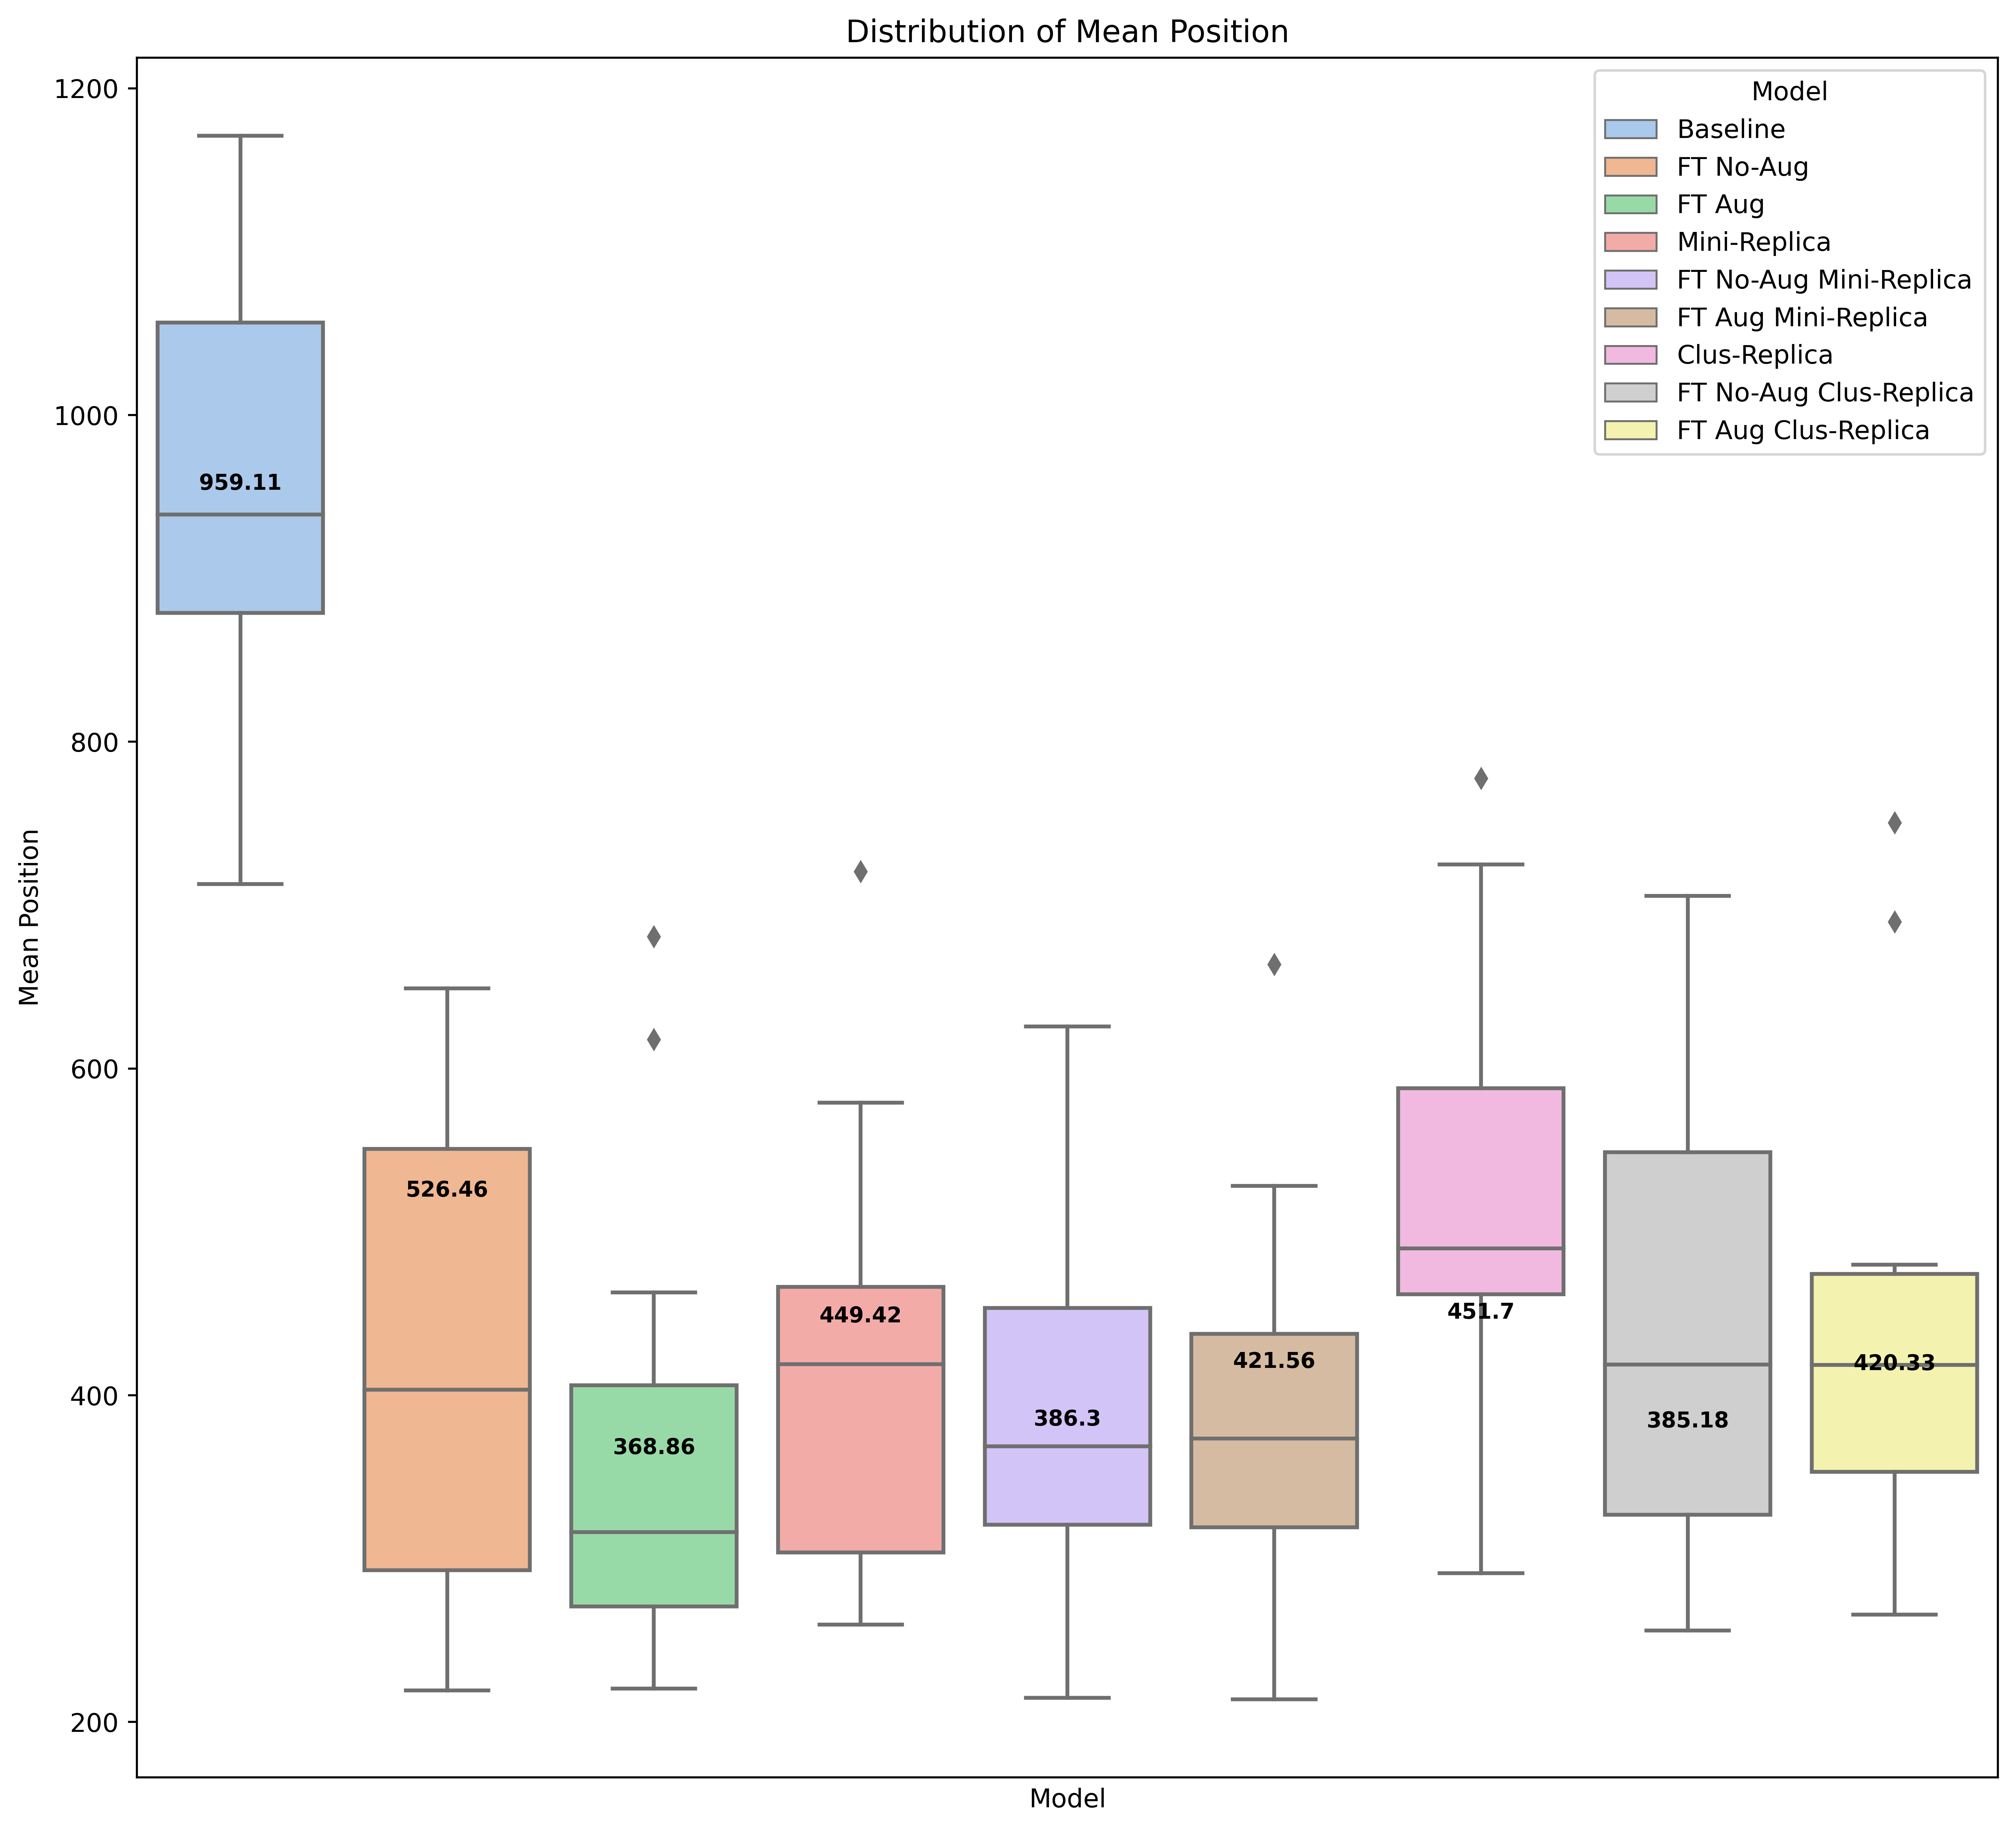
\includegraphics[width=\textwidth]{images/metrics/mp_test_data_500dpi.png}
      \caption{Mean Position comparison on Test data}
      \label{fig:test-data-mp}
\end{figure}

A deep learning model trains on examples, and in the cross-validation process, the model processes the samples in one of the two ways that impact the model. The training samples directly influence the step of updating the model parameters and those in the validation set to aid in adjusting the hyperparameters. Thus the performance measures of the model on the test set are central in providing an unbiased evaluation of the model. Consequently, the models discussed in Sections \ref{chap:5:sec:stle-aug} and \ref{chap:5:sec:ludo-models} are evaluated on the test sets to obtain an impartial assessment. Table \ref{tab:generalization-comp} presents the MAP and Recalls of the models averaged on 11 different data splits during the cross-validation, while Figure \ref{fig:test-data-mp} shows the distribution of the mean positions.

Fine-tuning the models significantly improves the ranking of the artworks similar to the drawings. While the ResNeXt-101 model fine-tuned only using the artwork drawing pairs reaches the lowest mean position, Mini-Replica achieves the highest recall and precision. The style augmentation of the drawings in training shows a notable effect on the results, and the generalization ability of such models is better than those trained otherwise. However, this effect is not apparent in the Clus-Replica model, and Chapter \ref{chap:6:Discussion} discusses it. Finally, these results on the test set establish that the models do not fit specific examples but learn low and high-level features that help construct a connection between the drawing and artwork.
